
\documentclass[12pt]{article}

\linespread{1.5}
\usepackage[margin=1.0in]{geometry}

\usepackage[nottoc]{tocbibind}
%\setcounter{secnumdepth}{3}

\usepackage{cite}
\usepackage{amsmath,amssymb,amsfonts}
\usepackage{algorithmic}
\usepackage{graphicx}
\usepackage{textcomp}
\usepackage{bm}
\usepackage{upgreek}

\usepackage{hyperref}

\usepackage{fancyhdr}
\pagestyle{fancy}
\fancyhf{}
\lhead{\leftmark}
\rfoot{\thepage}
\renewcommand{\headrulewidth}{2pt}
%\renewcommand{\footrulewidth}{1pt}

\usepackage[retainorgcmds]{IEEEtrantools}



%\graphicspath{ {C:/Users/Paul/Documents/PhD/Dissertation/Documentation/Figures/} }
\graphicspath{ {../Figures/} }


\DeclareMathOperator*{\argmin}{arg\,min}
\DeclareMathOperator*{\argmax}{arg\,max}

\DeclareMathOperator{\xrm}{\mathrm{x}}
\DeclareMathOperator{\Xrm}{\mathrm{X}}
\DeclareMathOperator{\yrm}{\mathrm{y}}
\DeclareMathOperator{\Yrm}{\mathrm{Y}}
\DeclareMathOperator{\Drm}{\mathrm{D}}
\DeclareMathOperator{\nrm}{\mathrm{n}}
\DeclareMathOperator{\nbarrm}{\bar{\mathrm{n}}}
\DeclareMathOperator{\zrm}{\mathrm{z}}
\DeclareMathOperator{\srm}{\mathrm{s}}
\DeclareMathOperator{\trm}{\mathrm{t}}

\DeclareMathOperator{\Prm}{\mathrm{P}}
\DeclareMathOperator{\prm}{\mathrm{p}}
\DeclareMathOperator{\Erm}{\mathrm{E}}
\DeclareMathOperator{\Crm}{\mathrm{C}}

\DeclareMathOperator{\Xcal}{\mathcal{X}}
\DeclareMathOperator{\Ycal}{\mathcal{Y}}
\DeclareMathOperator{\Dcal}{\mathcal{D}}
\DeclareMathOperator{\Ncal}{\mathcal{N}}
\DeclareMathOperator{\Zcal}{\mathcal{Z}}
\DeclareMathOperator{\Hcal}{\mathcal{H}}
\DeclareMathOperator{\Fcal}{\mathcal{F}}
\DeclareMathOperator{\Rcal}{\mathcal{R}}
\DeclareMathOperator{\Mcal}{\mathcal{M}}
\DeclareMathOperator{\Scal}{\mathcal{S}}
\DeclareMathOperator{\Pcal}{\mathcal{P}}
\DeclareMathOperator{\Lcal}{\mathcal{L}}
\DeclareMathOperator{\Tcal}{\mathcal{T}}

\DeclareMathOperator{\Rbb}{\mathbb{R}}
\DeclareMathOperator{\Nbb}{\mathbb{N}}
\DeclareMathOperator{\Zbb}{\mathbb{Z}}

\DeclareMathOperator{\Dir}{\mathrm{Dir}}
\DeclareMathOperator{\DM}{\mathrm{DM}}
\DeclareMathOperator{\Multi}{\mathrm{Multi}}
\DeclareMathOperator{\Bi}{\mathrm{Bi}}
\DeclareMathOperator{\DP}{\mathrm{DP}}
\DeclareMathOperator{\DMP}{\mathrm{DMP}}






\title{Qualifying Examination}
\author{Paul Rademacher}
%\date{}









\begin{document}

\maketitle

\newpage
\tableofcontents


\newpage
\section{Background} \label{sec:background}

The debate as to whether or not Bayesian approaches are suitable for statistical applications such as detection and estimation has a long history \cite{box}. For these well-established fields, many believe that the unknown element that statistically characterizes the observed data should not be treated as random, but rather as deterministic. This viewpoint is the foundation for a variety of classical inference methods that have been in use for decades. In estimation theory, the Cram\'er-Rao lower bound (CRLB) and Rao-Blackwell-Lehmann-Scheffe (RBLS) theorem provide solutions that are optimal (under certain conditions) \cite{kay-est}. In detection theory, the Neyman-Pearson theorem and generalized likelihood ratio test (GLRT) provide hypotheses without assigning probabilities to the underlying decision set \cite{kay-det}.

This distinction between deterministic and Bayesian methods in these traditional fields has been inherited by one of the fastest-growing scientific disciplines today: machine learning (ML). For \emph{supervised learning}, a set of input/output training observations is generated by an unknown probability function, or ``model'', and is then used to design a decision function which operates on novel inputs \cite{bishop}. The goal is to make decisions which tend to result in minimal ``loss'', which is measured by a user-defined function that compares each decision to the corresponding unobserved random element. Two of the most popular sub-topics in supervised learning are regression and classification, which naturally relate to estimation and detection. 

Most current supervised learning research is focused on the design of \emph{parametric} learning functions; that is, algorithms whose resultant decision functions can be characterized by a finite quantity of (typically real number) parameters. Of course, the attention on parametric learning is a consequence of the practicalities of real-world implementation - in our digital world, virtually all machine learning solutions are deployed on computers, and as such, they are bounded by the number of finite representations the computer memory can provide. However, as our computing capabilities continue to expand, so does our capacity to design higher-dimensional parametric learning functions.

Much of the popularity of and focus on machine learning today can be attributed to the resurgence of the multilayer perceptron and the success of deep neural networks (DNN) on classification challenges for speech and image recognition. Notable results include the successful application of deep belief networks to phone recognition on the TIMIT database \cite{mohamed} and deep convolutional neural networks (CNN) at the ImageNet Large Scale Visual Recognition Challenge (ILSVRC) 2010 \cite{krizhevsky}. By significantly improving upon the existing performance results at those times, widespread interest in new learning techniques was generated. Although the concept of the neural network has its roots in research as early as the 1950's, it wasn't until recently that we have had widespread access to computational power sufficient for training such large numbers of parameters on such voluminous collections of high-dimensional data. Many researchers credit the advances in computing and availability of large data sets as critical factors for these machine learning achievements.


Like other historically popular supervised learning algorithms, such as support vector machines (SVM) and decision trees, these deep learning algorithms do not derive from a Bayesian viewpoint. In fact, almost all of the highest profile machine learning approaches today are non-Bayesian. 


A common argument for why the unknown data model should not be treated as random is that there are often no environmental factors that suggest it is randomly generated. Although this justification is usually sound, the general application of Bayesian techniques is motivated by a different perspective: when the unknown element is treated as random and assigned a probability function, said function can simply be interpreted as a measure of the user's confidence in different data-generating models prior to any data being observed \cite{box}. The selection of this prior distribution is fundamental for Bayesian inference.

The success or failure of Bayesian learning methods hinge on how well the prior knowledge imparted by the designer matches reality. If a highly ``informative'' prior \cite{box} is chosen that is localized around the actual data probability distribution, low risk learning functions are possible even with limited training data; however, if the informative prior is poorly designed, a good solution may not be achieved. Conversely, a ``non-informative'' prior that weights the different distributions without preference provides a more robust solution for all models, but may under-perform relative to learners based on well-selected informative priors.

For many complex applications, designing a sensible prior distribution for Bayesian learning is challenging and often prohibitive. However, the wide range of learning functions afforded under the Bayesian perspective is valuable. In fact, many learning methods based on a deterministic treatment of the data-generating model have equivalents in Bayesian learning. This is prevalent among learning techniques that form point estimates of the data model via maximization, avoiding the potentially intractable integrations that are characteristic of full Bayesian learning methods.

Arguably the most widely used non-Bayesian technique for point estimation is the maximum likelihood (ML) method, with which the conditional distribution of the data given the model, or the ``likelihood function'', is maximized for the observed training set. The maximizing argument is treated as the true model and then used as a predictive distribution for novel observations \cite{theodoridis-ML}. The related Bayesian approach for model point estimation is the maximum \emph{a posteriori} (MAP) method, which utilizes a user-designed prior distribution to formulate the posterior distribution of the model given the training data; the maximizing model is then used as a point estimate. If the prior is uniform over its support (non-informative), then the MAP estimate is equivalent to the ML estimate.

Another example of equivalence between Bayesian and non-Bayesian learning methods is found in generalized squared-error regression applications. Commonly, the regressors parameters are designed using \emph{empirical risk minimization}, which is arguably the most common optimization metric for the design of classical and modern machine learning algorithms. It can be shown that the solution to this optimization is equivalent to ML estimation when the likelihood function is Gaussian with a mean value that is linearly dependent on the parameters. More interestingly, if the empirical risk objective is augmented with certain types of  regularizing terms, the resultant estimate is equivalent to a MAP estimate produced using a Gaussian prior over the regression parameters \cite{theodoridis-ML}. 

These examples illustrate that many classical estimation/learning methods, even without specifying a prior distribution, implicitly express a lack of \emph{a priori} model preference. Additionally, they highlight the flexibility of Bayesian learning methods, which can use both informative and non-informative prior distributions to control how decision functions trend with training data and how well they can perform for data-limited applications.














\section{Motivations} \label{sec:motivation}

The design of a parametric learning algorithm, either Bayesian or non-Bayesian, can be decomposed into two tasks: the specification of how the training data maps to the finite-dimensional parameter space and the specification of the parameters map to the higher-dimensional space of decision functions. The former is the ``learning'' procedure; the latter defines the mechanism for prediction. These two design tasks should be performed jointly, as the performance of a learning algorithm depends on both. However, it can be argued that the majority of current ML research directions are focused on the latter.


The notable modern successes of parametric machine learning algorithms, specifically deep learning approaches, and the widespread proliferation of open source code \cite{tensorflow} have made them an easy choice for many practitioners who are faced with a complex regression or classification application. Additionally, it can be argued that the lack of explainability of many of these methods and their ``black-box'' treatment has actually contributed to their dominance, rather than hindered it. 

Yet like all supervised learning approaches, they do not perform well for all problems. A basis for this principle was put forth by David Wolpert, who coined the ``No Free Lunch'' theorem (NFLT) \cite{wolpert}, which demonstrates that for any two learning approaches, there are as many problems for which the first outperforms the second as there are for which the second is superior. This theorem bears a critical query: what exactly about the design of these widely-used non-Bayesian algorithms makes them so effective for certain learning applications? As mentioned, the increased power of computing resources has enabled the training of higher-dimensional parameter spaces than ever before; however, the parameter adaptation operations most commonly selected, specifically empirical risk minimization, are not notably different from those used historically. Thus, to answer this question, the operations typically used by non-Bayesian ML functions for learning their parameters must be considered.

The failures of non-Bayesian methods are frequently attributed to a phenomenon termed ``overfitting''; that is, the failure of the learner to perform well on novel data not used during training. Overfitting is a direct result of empirical risk optimization, which attempts to minimize the aggregate loss assessed on the training samples. Interestingly, creating a design that performs well on the training data is straightforward - some of the simplest learning algorithms can achieve minimal empirical risk. For example, the nearest-neighbor algorithm simply classifies novel data by applying a distance measure, determining the ``nearest'' training sample, and copying the label; if the training samples are distinct, zero risk will be achieved \cite{devroye}. 

The overfitting issue underscores an important point: \emph{the empirical risk is not actually the objective function that the designer wants to minimize}. This is illustrated by the performance of nearest-neighbor on novel data, which suffers if the training data volume is insufficient. The desirable learner property is termed ``good generalization'' by non-Bayesians, but in truth this simply means that it achieves low \emph{expected risk} with respect to the unknown data-generating probability model. 

So if parameter training via empirical risk minimization does not guarantee generalization, why do modern non-Bayesian learning functions perform well? The answer must be strictly dependent on their pre-defined set of achievable functions. Parametric learning approaches, which account for nearly all popular algorithms, implicitly disallow the use of most of the complete function space and hopefully, any functions that lead to overfitting. Although no specific preference is given to any of the achievable functions in this subspace (assuming the empirical risk objective is not augmented with regularizing terms), the selection of this function subspace should be thought of as the imposition of \emph{prior knowledge}. From this perspective, even learning approaches that are widely deemed non-Bayesian can be seen from a Bayesian viewpoint.

This new perspective enables a Bayesian interpretation of all parametric learning methods. Again consider maximum likelihood, one of the most classic and well-established ``non-Bayesian'' learning approaches. Essentially all textbook examples of maximum likelihood establish a finite-dimensional subspace of the set of probability functions and then determine which model maximizes the likelihood function \cite{papoulis} - the selection of this subspace is critical to the efficacy of ML and should be viewed as user-imposed prior knowledge. Specifically, the ML estimate is equivalent to a MAP estimate based on a prior distribution that is uniform on a probability function subspace; this probability distribution is \emph{degenerate} and thus, highly informative.

If the user wanted a non-Bayesian approach that truly gave no preference to any data-generating model, the full set of probability distributions should be used. In this case, the ML method would show that the most likely model would be the \emph{empirical distribution} generated from the training data \cite{rao}. The use of such a point estimate for novel predictions would dictate the use of the empirical risk metric. While it can be shown that empirical risk minimization is equivalent to expected risk minimization in the limit of training data volume, in the practical scenario of limited training data all the overfitting phenomena previously discussed will again be of issue. 

This point suggests that the use of prior knowledge is \emph{mandatory} for effective machine learning on most applications - the user must impose structure for the optimization routine to produce a high performance decision function. For non-probabilistic approaches to parametric supervised learning (neural networks, support vector machines, decision trees, etc.), the prior knowledge is imparted via the specific mapping from the parameter space directly to the decision function space. For Bayesian parametric learning, the prior knowledge maps the parameter space to the full space of probability distributions, which then determines the optimal decision function. 

The mapping from the learned parameters to the decision function subspace becomes increasingly important for applications where the parameter space is of significantly lower dimensionality than the complete training data space; this is commonly referred to as ``dimensionality reduction''. While algorithms that learn from low-dimensional data can define enough parameters to guarantee retention of all statistically informative data components, those operating on high-dimensional data will typically have no practical option but to transform the data into compact features. 

This is the case for many human recognition tasks of interest for machine learning research. Consider image recognition. A single 8-bit RGB (red, green, blue) pixel has over 16 million possible values, a moderate image size is 256-by-256 pixels, and some image databases can have over 10's of millions of labeled images - the amount of digital memory needed to represent such a training set is enormous. Consequently, the data is compressed by a massive factor, forming the learned parameters. 

Although dimensionality reduction of training data is generally sub-optimal, for high-dimension tasks such as these it is also sensible. Despite the increased availability of training data for modern machine learning algorithms, the data space is still critically under-sampled; this is sometimes referred to as the ``curse of dimensionality'' \cite{bellman}. From this viewpoint, highly informative prior knowledge is a must for low-risk predictions. Significant dimensionality reduction of the training data, if well conceived, will reflect a strong prior understanding of the data statistics and which transforms will preserve the underlying information. 














\section{Problem Statement} \label{sec:prob}

The goal of the thesis will be to investigate how a user's prior knowledge can be best exploited for the design of parametric decision functions for supervised machine learning. The initial research will focus on applications where the joint set that an observed/unobserved datum is drawn from is finite; this will enable a simpler analysis of the role of dimensionality reduction in the selection of the finite-dimension function space.

As the prior knowledge used to define a learning algorithm is necessarily human-generated, the techniques developed in this thesis will specifically focus on regression and classification applications that mimic human prediction/recognition tasks. For example, speech recognition and image recognition algorithms are motivated by the desire to automate jobs typically performed by humans. Despite the recent advances in machine learning performance on such tasks, machines have yet to match the capabilities of their human counterparts.



\subsection{Data Model and Objective}

Consider an observable random element $\xrm \in \Xcal$ and and unobservable random element $\yrm \in \Ycal$ which are jointly distributed according to an unknown probability distribution $\uptheta \in \Theta = \Pcal(\Ycal \times \Xcal)$, such that $\Prm_{\yrm,\xrm | \uptheta} = \uptheta$. Note that the uppercase PMF notation used throughout this section implies that the random elements are discrete; PDF's are used when $\xrm$ and/or $\yrm$ are continuous random variables/processes.

Also observed is a random sequence of $N$ samples from $\uptheta$, denoted $\Drm \in \Dcal = \{\Ycal \times \Xcal\}^N$; an alternative representation that can be used is $\Drm \equiv ( \Yrm,\Xrm )$. The $N$ data pairs are conditionally independent from one another and are identically distributed as $\Prm_{\Drm_n | \uptheta} = \uptheta$. The samples are also conditionally independent from $(\yrm,\xrm)$. Thus,
\begin{equation}
\Prm_{\yrm,\xrm,\Drm | \uptheta}(y,x,D | \theta) = \Prm_{\yrm,\xrm | \uptheta}(y,x | \theta) \prod_{n=1}^N \Prm_{\Drm_n | \uptheta}\big(Y_n,X_n | \theta\big) \;.
\end{equation}

The task in supervised machine learning is to design a decision function $f: \Dcal \mapsto \Hcal^{\Xcal}$ which produces a mapping from the space of the observed random elements to a decision space $\Hcal$. Define the function space $\Fcal = \left\{ {\Hcal^{\Xcal}} \right\}^{\Dcal}$, such that $f \in \Fcal$. The learning functions are non-parametric and there are no restrictions on the set of achievable functions $\Fcal$.

The metric guiding the design is a loss function $\Lcal: \Hcal \times \Ycal \mapsto \Rbb_{\geq 0}$ which penalizes the decision $h \in \Hcal$ based on the value of $\yrm$. The objective is to minimize the conditional expected loss, or conditional ``risk'',
\begin{IEEEeqnarray}{rCl} \label{eq:risk_cond}
\Rcal_{\Theta}(f ; \uptheta) & = &  \Erm_{\yrm,\xrm,\Drm | \uptheta} \Big[ \Lcal\big( f(\xrm;\Drm),\yrm \big) \Big] \\
& = & \Erm_{\Drm | \uptheta}\Bigg[ \Erm_{\xrm | \uptheta}\bigg[ \Erm_{\yrm | \xrm,\uptheta}\Big[ \Lcal\big( f(\xrm;\Drm),\yrm \big) \Big] \bigg] \Bigg] \nonumber \;.
\end{IEEEeqnarray}
where the conditional independence of random element $\yrm$ from the training data $\Drm$ given the model $\uptheta$ is used. As the model $\uptheta$ is not observed, $\Rcal_{\Theta}: \Theta \mapsto {\Rbb_{\geq 0}}^{\Fcal}$ is not a feasible objective function for optimization. This is the fundamental challenge of supervised learning: the true risk objective is unknown and the designer can never be precisely sure how well any decision function performs. 







\subsubsection{Clairvoyant Decision}

It is informative to formulate the optimal decision function assuming the model $\uptheta$ was in fact observed; it will be referred to as the ``clairvoyant'' function, following terminology used in \cite{kay-det}. This clairvoyant decision function $f_{\Theta}: \Theta \mapsto \Fcal$ is represented by
\begin{equation}
f_{\Theta}(\uptheta) = \argmin_{f \in \Fcal} \Rcal_{\Theta}(f ; \uptheta) \;.
\end{equation}
For a given set of observations $\xrm$ and $\Drm$, the function $f_{\Theta}(\uptheta) \in \Fcal$ selects the decision $h = \argmin_{h \in \Hcal} \Erm_{\yrm | \xrm,\uptheta}\big[ \Lcal(h,\yrm) \big]$. Note the conditional independence of $\yrm$ from $\Drm$ in \eqref{eq:risk_cond} - the knowledge of $\uptheta$ renders the training data $\Drm$ uninformative. As such, the range of the clairvoyant function is recast as $f_{\Theta} : \Theta \mapsto \Hcal^{\Xcal}$ and the decisions are
\begin{equation} \label{eq:f_clv_x}
f_{\Theta}(\xrm;\uptheta) = \argmin_{h \in \Hcal} \Erm_{\yrm | \xrm,\uptheta}\big[ \Lcal(h,\yrm) \big] \;.
\end{equation}
The corresponding clairvoyant risk for a given model $\uptheta$ is
\begin{IEEEeqnarray}{rCl} \label{eq:risk_clv}
\Rcal_{\Theta}^*(\uptheta) & \equiv & \Rcal_{\Theta}\big( f_{\Theta}(\uptheta) ; \uptheta \big) \\
& = & \min_{f \in \Fcal} \Rcal_{\Theta}(f ; \uptheta) \nonumber \\
& = & \Erm_{\xrm | \uptheta} \left[ \min_{h \in \Hcal} \Erm_{\yrm | \xrm,\uptheta}\big[ \Lcal(h,\yrm) \big] \right] \nonumber \;.
\end{IEEEeqnarray}






\subsubsection{Bayes Decision}

To design an optimal decision function $f \in \Fcal$, an operator must be chosen to remove the dependency of the conditional risk on $\uptheta$ and form an objective function $\Fcal \mapsto \Rbb_{\geq 0}$. One choice is to integrate over $\Theta$; to ensure a non-negative objective value, the weighting function should be non-negative. Also, as scaling the objective function will not change its minimizing argument, the weighting function can be constrained to integrate to one. These are the requirements for a valid probability density function (PDF); as such, the model $\uptheta$ is treated as a random process and a Bayesian approach can be adopted. 

Define the PDF $\prm_{\uptheta} \in \Pcal(\Theta)$. Now the Bayes risk can be formulated as
\begin{IEEEeqnarray}{rCl} \label{eq:risk}
\Rcal(f) & = & \Erm_{\uptheta}\big[ \Rcal_{\Theta}(f ; \uptheta) \big] \\
& = & \Erm_{\yrm,\xrm,\Drm}\big[ \Lcal(f(\xrm;\Drm),\yrm) \big] \nonumber \\
& = & \Erm_{\Drm}\Bigg[ \Erm_{\xrm | \Drm}\bigg[ \Erm_{\yrm | \xrm,\Drm} \Big[ \Lcal\big( f(\xrm;\Drm),\yrm \big) \Big] \bigg] \Bigg] \nonumber
\end{IEEEeqnarray}
and $\yrm$, $\xrm$, and $\Drm$ are treated as jointly distributed random elements. Observe that the Bayesian predictive distributions can be represented as $\Prm_{\xrm | \Drm} = \Erm_{\uptheta | \Drm}\big[ \Prm_{\xrm | \uptheta} \big]$ and $\Prm_{\yrm | \xrm,\Drm} = \Erm_{\uptheta | \xrm,\Drm}\big[ \Prm_{\yrm | \xrm,\uptheta} \big]$, the expected values of the corresponding clairvoyant distributions with respect to the model posteriors $\prm_{\uptheta | \Drm}$ and $\prm_{\uptheta | \xrm,\Drm}$, respectively.

Finally, express the optimal learning function
\begin{equation} 
f^* = \argmin_{f \in \Fcal} \Rcal(f) \;.
\end{equation}
The decision expressed by the learning function $f^*$ given observed values of $\xrm$ and $\Drm$ is
\begin{IEEEeqnarray}{rCl} \label{eq:f_opt_xD}
f^*(\xrm;\Drm) & = & \argmin_{h \in \Hcal} \Erm_{\yrm | \xrm,\Drm}\big[ \Lcal(h,\yrm) \big] \\
& = & \argmin_{h \in \Hcal} \Erm_{\uptheta | \xrm,\Drm}\bigg[ \Erm_{\yrm | \xrm,\uptheta}\big[ \Lcal(h,\yrm) \big] \bigg] \nonumber \;.
\end{IEEEeqnarray}
Thus, the Bayesian approach uses the model posterior $\prm_{\uptheta | \xrm,\Drm}$ to integrate out the dependency on the model given the observable random elements. The minimum Bayes risk is
\begin{IEEEeqnarray}{rCl} \label{eq:risk_min}
\Rcal^* & \equiv & \Rcal(f^*) \\
 & = & \min_{f \in \Fcal} \Rcal(f) \nonumber \\
& = & \Erm_{\Drm} \Bigg[ \Erm_{\xrm | \Drm} \bigg[ \min_{h \in \Hcal} \Erm_{\yrm | \xrm,\Drm}\big[ \Lcal(h,\yrm) \big] \bigg] \Bigg] \nonumber \;.
\end{IEEEeqnarray}






\subsection{Applications to Common Loss Functions}

In this section, loss functions typical for classification and regression applications, specifically the 0-1 loss function and the squared-error loss function, are adopted. The conditional risk \eqref{eq:risk_cond} is assessed, clairvoyant learners \eqref{eq:f_clv_x} are found, and the clairvoyant risk \eqref{eq:risk_clv} is expressed.


\subsubsection{Regression: the Squared-Error Loss}

The squared-error (SE) loss function is arguably the most commonly used loss function for regression, or in fact for any estimation problem. This can be attributed to its quadratic form, which enables a closed-form expression of the minimizing estimation function.

It is assumed that the unobserved random element $\yrm$ is a scalar random variable; that is, $\Ycal \subseteq \Rbb$. Additionally, the learning function's estimate is allowed to assume real numbers; thus, $\Hcal = \Rbb \supseteq \Ycal$.

The loss function is defined as
\begin{equation}
\Lcal(h,y) = (h-y)^2 \;.
\end{equation}
Substituting the squared-error loss into \eqref{eq:risk_cond}, the conditional squared-error risk is
\begin{IEEEeqnarray}{rCl} \label{eq:risk_cond_SE}
\Rcal_{\Theta}(f ; \uptheta) & = & \Erm_{\xrm | \uptheta}\Bigg[ \Erm_{\yrm| \xrm,\uptheta}\bigg[ \Erm_{\Drm | \uptheta}\Big[ \big( f(\xrm;\Drm)-\yrm \big)^2 \Big] \bigg] \Bigg] \\
& = & \Erm_{\xrm | \uptheta} \left[ \Sigma_{\yrm | \xrm,\uptheta} \right] + \Erm_{\xrm,\Drm | \uptheta} \Big[ \big( f(\xrm;\Drm) - \mu_{\yrm | \xrm,\uptheta} \big)^2 \Big] \nonumber \;,
\end{IEEEeqnarray}
a sum of two terms. The first term is the expected conditional variance of the true predictive distribution $\Prm_{\yrm | \xrm,\uptheta}$. The second term is the expected squared bias between the Bayesian estimate and the true mean $\mu_{\yrm | \xrm,\uptheta}$.





\paragraph{Clairvoyant Estimation}

To find the clairvoyant estimator, the squared-error loss is substituted into \eqref{eq:f_clv_x}; note that the objective function is quadratic over the argument $h \in \Hcal = \Rbb$. It is easily shown that the function over $h$ is positive-definite; as such, the minimizing decision $h$ is the sole stationary point. Setting the first derivative of the function to zero, the clairvoyant estimate is the expected value of $\yrm$ given the model $\uptheta$ and the observed value $\xrm$, such that
\begin{IEEEeqnarray}{rCl} \label{eq:f_clv_SE}
f_{\Theta}(\xrm;\uptheta) & = & \argmin_{h \in \Rbb} \Erm_{\yrm | \xrm,\uptheta} \left[ (h-\yrm)^2 \right] \\
& = &  \mu_{\yrm | \xrm,\uptheta} \nonumber \;.
\end{IEEEeqnarray}
Substituting the loss and clairvoyant function into \eqref{eq:risk_clv}, the resulting clairvoyant risk is
\begin{IEEEeqnarray}{rCl}
\Rcal_{\Theta}^*(\uptheta) & = & \Erm_{\xrm | \uptheta} \Big[ \Erm_{\yrm | \xrm,\uptheta} \big[ (\yrm - \mu_{\yrm | \xrm,\uptheta})^2 \big] \Big] \\
& = & \Erm_{\xrm | \uptheta} \left[ \Sigma_{\yrm | \xrm,\uptheta} \right] \nonumber \;.
\end{IEEEeqnarray}

Observe that the general conditional risk \eqref{eq:risk_cond_SE} can be represented as $\Rcal_{\Theta}(f ; \uptheta) = \Rcal_{\Theta}^*(\uptheta) + \Erm_{\xrm,\Drm | \uptheta} \Big[ \big( f(\xrm;\Drm) - f_{\Theta}(\xrm;\uptheta) \big)^2 \Big]$. The first summand is equal to the clairvoyant squared-error; the second term is dependent on the difference between the general estimate and the clairvoyant estimate. Figure \ref{fig:Risk_clv_SE} displays the clairvoyant risk for models $\theta(\cdot,x)$ independent of $x$. 
\begin{figure}
\centering
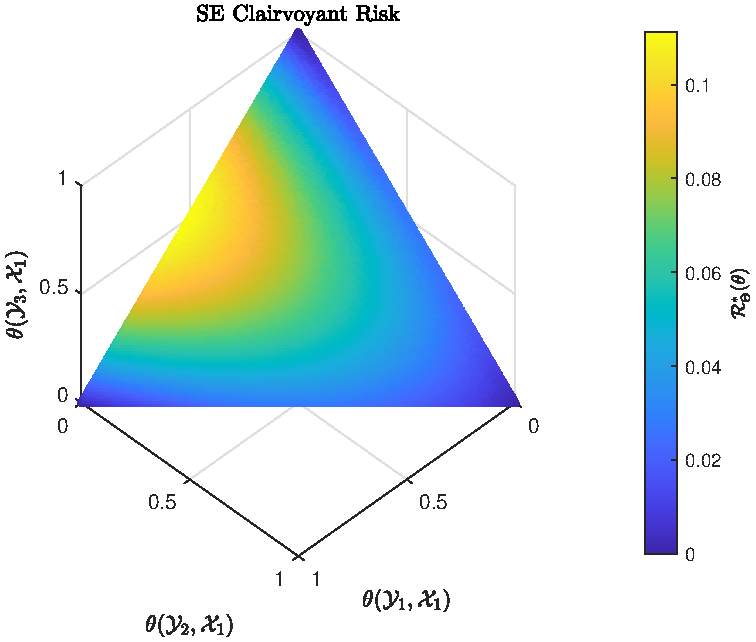
\includegraphics[width=0.7\linewidth]{Risk_clv_SE.pdf}
\caption{Clairvoyant Risk for the Squared-Error Loss Function, constant $\theta(\cdot,x)$}
\label{fig:Risk_clv_SE}
\end{figure}






\paragraph{Bayesian Estimation}

To find the optimal estimator, the squared-error loss is substituted into \eqref{eq:f_opt_xD}. Again, the function over $h$ is positive-definite; as such, the minimizing decision $h$ is the sole stationary point. Setting the first derivative of the function to zero, the optimal estimate is the expected value of $\yrm$ given the training data and the observed value $\xrm$, such that
\begin{IEEEeqnarray}{rCl} \label{eq:f_opt_SE}
f^*(\xrm;\Drm) & = & \argmin_{h \in \Rbb} \Erm_{\yrm | \xrm,\Drm} \left[ (h-\yrm)^2 \right] \\
& = & \mu_{\yrm | \xrm,\Drm} = \Erm_{\uptheta | \xrm,\Drm} \left[ \mu_{\yrm | \xrm,\uptheta} \right] \nonumber \;.
\end{IEEEeqnarray}

An interesting form for the optimal estimator is $f^*(\xrm;\Drm) = \Erm_{\uptheta | \xrm,\Drm} \big[ f_{\Theta}(\xrm;\uptheta) \big]$. Substituting the squared-error loss into the second line of \eqref{eq:f_opt_xD}, the optimal Bayes estimator is the condtional expected value of the clairvoyant estimate with respect to the model posterior distribution.



The Bayes squared-error risk for a general learning function is
\begin{IEEEeqnarray}{rCl} \label{eq:risk_SE}
\Rcal(f) & = & \Erm_{\uptheta} \Bigg[ \Erm_{\Drm | \uptheta} \bigg[ \Erm_{\yrm,\xrm | \uptheta} \Big[ \big( f(\xrm;\Drm)-\yrm \big)^2 \Big] \bigg] \Bigg] \\
& = & \Erm_{\uptheta}\big[\Rcal_{\Theta}^*(\uptheta)\big] + \Erm_{\xrm,\Drm,\uptheta} \Big[ \big( f(\xrm;\Drm) - \mu_{\yrm | \xrm,\uptheta} \big)^2 \Big] \nonumber \\
& = & \Erm_{\xrm,\Drm} \left[ \Sigma_{\yrm | \xrm,\Drm} \right] + \Erm_{\xrm,\Drm} \Big[ \big( f(\xrm;\Drm) - \mu_{\yrm | \xrm,\Drm} \big)^2 \Big] \nonumber \;.
\end{IEEEeqnarray}

Substituting the optimal estimator \eqref{eq:f_opt_SE} into Equation \eqref{eq:risk_SE}, the minimum Bayes risk is the expected conditional variance
\begin{IEEEeqnarray}{rCl} \label{eq:risk_min_SE}
\Rcal^* & = & \Erm_{\xrm,\Drm} \left[ \Sigma_{\yrm | \xrm,\Drm} \right] \\
& = & \Erm_{\xrm,\uptheta} \left[ \Sigma_{\yrm | \xrm,\uptheta} \right] + \Erm_{\xrm,\Drm} \left[ \Crm_{\uptheta | \xrm,\Drm} \left[ \mu_{\yrm | \xrm,\uptheta} \right] \right] \nonumber \;.
\end{IEEEeqnarray}
The first term is the irreducible risk. The second term is the expected variance of the clairvoyant estimate $f_{\Theta}(\xrm;\uptheta) = \mu_{\yrm | \xrm,\uptheta}$ with respect to the model posterior PDF $\prm_{\uptheta | \xrm,\Drm}$





\subsubsection{Classification: the 0-1 Loss}

In this section, the developed framework is applied to a common machine learning task: classification. In classification problems, the set $\Ycal$ is countable and typically finite. Furthermore, the hypothesis space is usually identical to the unobserved variable space; that is $\Hcal = \Ycal$. The 0-1 loss function is the most widely used for these problems; it is represented as
\begin{equation} \label{eq:loss_01}
\Lcal(h,y) = 1 - \delta[h,y] \;.
\end{equation}
Applying the 0-1 loss, the conditional risk \eqref{eq:risk_cond} for a general classifier is
\begin{IEEEeqnarray}{rCl} \label{eq:risk_cond_01}
\Rcal_{\Theta}(f ; \uptheta) & = & 1 - \Erm_{\Drm | \uptheta} \bigg[ \Erm_{\yrm,\xrm | \uptheta} \Big[ \delta\big[ f(\xrm;\Drm),\yrm \big] \Big] \bigg] \\
& = & 1 - \sum_{x \in \Xcal} \Erm_{\Drm | \uptheta} \Big[ \uptheta\big( f(x;\Drm),x \big) \Big] \nonumber \;.
\end{IEEEeqnarray}





\paragraph{Clairvoyant Hypothesis}

To find the clairvoyant classifier, the 0-1 loss is substituted into \eqref{eq:f_clv_x}; given an observation $x$, the optimum hypothesis is simply the value $y$ that maximizes the conditional model $\tilde{\uptheta}(x)$,
\begin{IEEEeqnarray}{rCl} \label{eq:f_clv_01}
f_{\Theta}(\xrm;\uptheta) & = & \argmin_{h \in \Ycal} \Erm_{\yrm | \xrm,\uptheta} \left[ 1 - \delta[h,y] \right] \\
& = & \argmax_{h \in \Ycal} \Prm_{\yrm | \xrm,\uptheta}(h | \xrm,\uptheta) \nonumber \\
& = & \argmax_{y \in \Ycal} \uptheta(y,\xrm) \nonumber \;.
\end{IEEEeqnarray}
Substituting the 0-1 loss and clairvoyant hypothesis into \eqref{eq:risk_clv}, the resulting clairvoyant risk is
\begin{IEEEeqnarray}{rCl}
\Rcal_{\Theta}^*(\uptheta) & = & 1 - \Erm_{\xrm | \uptheta} \Big[ \max_{y \in \Ycal} \Prm_{\yrm | \xrm,\uptheta}(y | \xrm,\uptheta) \Big] \\
& = & 1 - \sum_{x \in \Xcal} \max_{y \in \Ycal} \uptheta(y,x) \nonumber \;.
\end{IEEEeqnarray}

Figure \ref{fig:Risk_clv_01} displays the clairvoyant risk for models $\theta(\cdot,x)$ independent of $x$. Intuitively, the models that are more concentrated lead to lower probability of error.
\begin{figure}
\centering
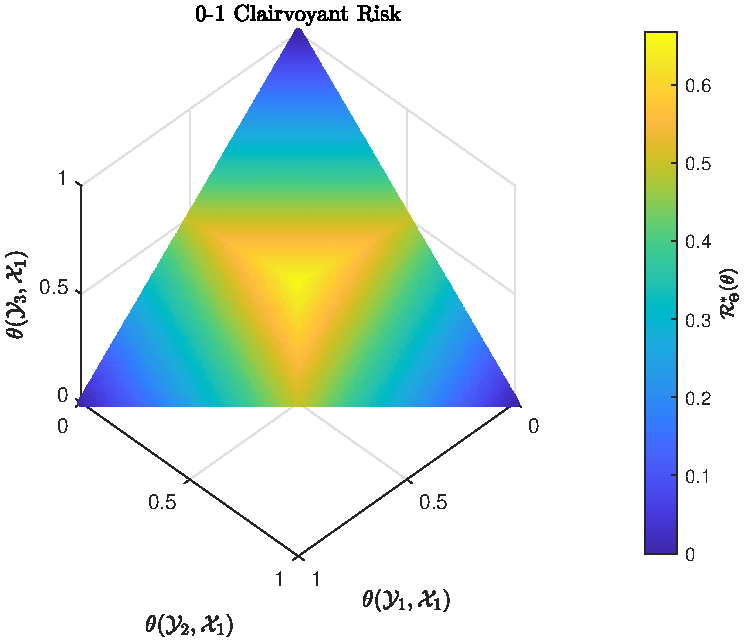
\includegraphics[width=0.7\linewidth]{Risk_clv_01.pdf}
\caption{Clairvoyant Risk for the 0--1 Loss Function, constant $\theta(\cdot,x)$}
\label{fig:Risk_clv_01}
\end{figure}



\paragraph{Bayesian Hypothesis}

To determine the optimal Bayesian classification function, the 0-1 loss from Equation \eqref{eq:loss_01} is substituted into Equation \eqref{eq:f_opt_xD} to find
\begin{IEEEeqnarray}{rCl} \label{eq:f_opt_01}
f^*(\xrm;\Drm) & = & \argmin_{h \in \Ycal} \Erm_{\yrm | \xrm,\Drm}\big[ 1 - \delta[h,\yrm] \big] \\
& = & \argmax_{y \in \Ycal} \Prm_{\yrm | \xrm,\Drm}(y | \xrm,\Drm) \nonumber \;.
\end{IEEEeqnarray}
The optimal classifier chooses the value $y \in \Ycal$ that maximizes the Bayesian predictive PMF for the observed values of $\xrm$ and $\Drm$.


Using the 0-1 loss, the minimum Bayes probability of error \eqref{eq:risk_min} is
\begin{IEEEeqnarray}{rCl} \label{eq:risk_01}
\Rcal(f) & = & 1 - \Erm_{\xrm,\Drm} \left[ \Prm_{\yrm | \xrm,\Drm}\big( f(\xrm;\Drm) | \xrm,\Drm \big) \right] \;.
\end{IEEEeqnarray}

Substituting the optimal learner \eqref{eq:f_opt_01} into the general risk \eqref{eq:risk_01}, the minimum probability of error is 
\begin{IEEEeqnarray}{rCl} \label{eq:risk_min_01}
\Rcal^* & = & 1 - \Erm_{\xrm,\Drm} \left[ \max_{y \in \Ycal} \Prm_{\yrm | \xrm,\Drm}(y | \xrm,\Drm) \right] \;.
\end{IEEEeqnarray}






\subsection{Application to Human Recognition Tasks}

Human recognition abilities are certainly remarkable, and can in part be attributed to the immeasurable volume of ``training data'' that we consume during our lives. However, individual humans must be said to have a type of ``prior knowledge'' even before being born - all healthy human beings pre-process our multi-sensory input in essentially the same way and assess similarities between observations using the same metrics. 


This pre-processing undoubtedly exploits the highly structured nature of our sensory records. Consider visual recognition. Not only do we only process a fraction of the electromagnetic spectrum, but the matter off of which our received energy reflects is highly structured. To underscore this point, consider the uniformly randomly generated RGB image in Figure \ref{fig:RGB_random}, which could never be mistaken for an image recorded from the visual spectrum. Indeed, the space of sensible RGB images for visual recognition only comprises a minuscule fraction of the complete RGB image space. 
\begin{figure}
\centering
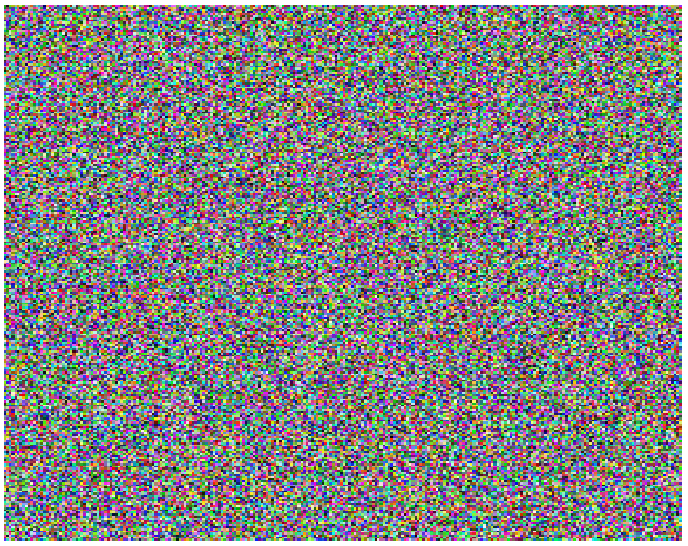
\includegraphics[width=0.5\linewidth]{RGB_random.pdf}
\caption{Randomly generated RGB image}
\label{fig:RGB_random}
\end{figure}

It may also be said that all humans possess a mechanism for ``dimensionality reduction'' - our mental records of our observations are not complete, but rather are represented by a compact set of descriptors. Understanding these ``feature extraction'' procedures performed by our sensory organs has been a research interest for those seeking to improve the automation of human recognition. 


Another important perspective regarding how humans make predictions is that the labels we use are almost always \emph{extrinsic} to the physical world. That is, the categories we use to describe things are of our own design - in fact, much of our internal classification procedure can be thought of as \emph{unsupervised learning}. To exemplify this, consider speech recognition. Spoken ``words'' are nothing more than fluctuations of air pressure, but we use man-made descriptors to efficiently represent the distinct patterns we emit. In image recognition on ImageNet \cite{krizhevsky}, different images are labeled as ``container ships'' or ``lifeboats''; this distinction is man-made as well.

From this point of view, it should be unsurprising that humans outperform machines on these recognition tasks - we defined the classes ourselves, ensuring joint class-data probability distributions that lead to minimal risk. With sufficient prior knowledge, parametric decision functions that meet these levels of performance should be realizable. To illustrate this point, consider the handwritten digit samples \cite{lecun-mnist} shown in Figure \ref{fig:mnist_digit_ex}. Undoubtedly, most human observers will have no problem accurately classifying all of these samples. 
\begin{figure}
\centering
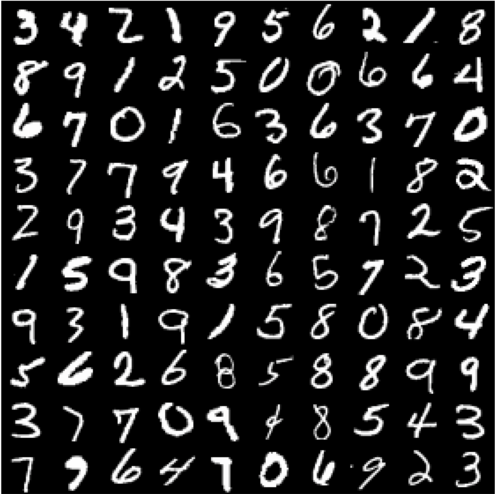
\includegraphics[width=0.5\linewidth]{mnist_digit_ex.png}
\caption{Handwritten digit samples from the MNIST Database}
\label{fig:mnist_digit_ex}
\end{figure}











\section{Related Work} \label{sec:related}

\subsection{Statistical Learning}

Supervised learning has a long history pre-dating the widespread acceptance of the newly popular phrase ``machine learning''. Such a broad technical area inescapably spans a variety of fields - learning theory is of theoretical interest in applied mathematics and statistics and it has found practical interest for applications in electrical engineering and computer science. 

Many important results in supervised learning theory come from a statistical foundation. Fundamental questions about the existence of asymptotically consistent estimators have found their answers in the works of researchers including Stone \cite{stone}, who first studied the consistency of the k-nearest neighbor classification rule. In 1971, Vapnik and Chervonenkis set down theory on empirical risk minimization \cite{vapnik}, providing bounds on the risk achievable by a classifier when it is restricted to a specific group of functions. Although works such as these are not typically considered ``Bayesian'', they do implicitly underscore the importance of restricting the design of the decision function to a limited function space, especially when the empirical risk objective drives the design.

Non-Bayesian treatments of statistical inference such as these commonly provide results in the form of asymptotic trends for large sample sizes or as risk lower bounds \cite{devroye}. However, not as much is offered in the way of practical solutions for limited volumes of data - this is where the Bayesian perspective is most valuable. Since the Bayes theorem was put forth by Bayes himself in 1763 \cite{bayes}, interest in a Bayesian approach to statistical inference has waned and waxed. The varying popularity of these methods can be attributed in part to a philosophical belief that prior assumptions degraded the information inferred from the data alone; additionally, the computational burden of Bayesian methods (via approximations of integrals) made them unattractive compared to classical methods \cite{box}.

While modern advances in computing have made Bayesian techniques more applicable to a variety of problems, the computational challenges inherent to Bayesian inference persist. Many modern research directions on Bayesian learning attempt to move away from the most tractable (and most presumptuous) methods, such as those that assume Gaussian data distributions, while still providing computational methods for practical implementation. Such methods will likely have relevance for this thesis, especially for Bayesian learners based on priors with low-dimensional support sets.

One of the more popular approaches is to use a \emph{hierarchical prior}, which defines the data-generating model in terms of other unknown ``latent variables'', or hyperparameters, and then remove the dependency on the model with a single procedure. An example is the expectation-maximization (EM) algorithm \cite{dempster}, which performs an alternating optimization by iteratively evaluating expectations of the data likelihood function and then forming maximum likelihood estimates of the model hyperparameters; after convergence, the point estimates of the hyperparameters are used to formulate the model posterior and inferences are made as usual. This algorithm is widely used for Gaussian mixture models (GMM's) in clustering applications.

Use of the EM algorithm requires the model posterior given the observed data. When evaluation of the model posterior is intractable, different methods must be used - a significant portion of research on Bayesian methods focuses on overcoming this difficulty. Approximate inference methods are one such class of solutions. With variational approximation, the EM algorithm can be approximated by forming an estimate of the posterior from a class of distributions that enables a tractable solution \cite{beal}. Another alternative is the expectation propagation algorithm \cite{minka-ep}, which estimates the posterior by performing an optimization on the Kullback-Leiber divergence metric. Non-deterministic methods are also popular for approximate inference, using random sampling to approximate expectations; some notable approaches are importance sampling \cite{mackay-is} and Markov chain Monte Carlo (MCMC) methods, including the Metropolis-Hastings algorithm \cite{hastings}. These approximation methods will be used as necessary for Bayesian learning with limited-support priors.


Use of the Dirichlet distribution for Bayesian inference is typically found in non-parametric learning by way of the continuous Dirichlet process \cite{ferguson}. The most common use is for unsupervised learning applications, specifically clustering with infinite numbers of clusters \cite{gershman}. For supervised learning, however, most current research on Bayesian learning from data drawn from continuous sets uses Gaussian processes \cite{rasmussen,meeds} to weight decision functions rather than the data-generating probability distributions.



\subsection{Human Recognition Features}

Existing research on human recognition is extensive; some related works focusing on feature extraction may be used to guide design Bayesian methods for this thesis. 

In speech recognition, feature design is motivated by investigations suggesting that the human auditory system performs a real-time spectral analysis \cite{rabiner} of its input. Furthermore, the frequency information is processed on a logarithmic scale \cite{flanagan}; this perspective has motivated the widespread adoption of features like the Mel frequency cepstral coefficients (MFCC's) \cite{picone}, which attempt to compress signals into a lower-dimensional space for word/phoneme classification. Similarly, for image recognition, work by Campbell \cite{campbell-orientation,campbell-fourier} uses a Fourier-based signal decomposition to isolate informative signal components; for example, visual images contain most of their energy in low-frequency Fourier coefficients. 

Both of these human recognition highlight the inclination of our sensory processing systems to decompose information in a variety of ways and at a variety of scales. This observation underscores the benefit of using features based on a multiresolution signal decomposition. In particular, the family of wavelet representations \cite{mallat-wavtour} are popular for these learning applications; a wide range of interesting research directions, including multiscale edge detection and curvelet approximation, have provided features for efficient signal description. 

Our understanding of certain human sensory processes has led to specialized signal transformations that overcome undesirable effects in more standard feature extraction. For example, in optical character recognition (OCR) (and in fact for most human recognition tasks), the translation dependency of a feature can be significantly raise the probability of error. Reconciling our desire for features that describe spatial locality with the need for translation-invariant representation is challenging - even popular features such as those based on multiresolution wavelet transformations \cite{mallat-multires} do not provide both. Focused research on shift-invariant features for 2-dimensional data \cite{marco} aims to ensure this property and provide learning algorithms with features that well approximate those utilized in our own cognition.






\section{Approach} \label{sec:approach}

Having motivated the perspective that \emph{all} machine learning algorithms either implicitly or explicitly use prior knowledge, this thesis will focus on a strictly Bayesian approach to parametric supervised learning. Many existing treatments of Bayesian machine learning only address parametric learners, which reduce the data dimensionality, and yet fail to sufficiently consider the implications of how the mapping between the finite set of parameters and the probability model is selected. As such, the  framework set down previously will be used; it is general enough to accommodate learning designs based on any prior distribution, even those with full support over potentially infinite-dimensional function spaces. Designs using both full and limited dimensionality prior distributions will be considered for application to human recognition tasks.




\subsection{Model and Data Transformations}

To simplify the analyses, the model $\uptheta$ and the training data $\Drm$ will be frequently interpreted with alternate representations. The model $\uptheta$ is split into conditional and marginal distributions using a bijective transformation. The training data is compressed into the empirical distribution, a sufficient statistic for the model; this empirical distribution is decomposed into ``conditional'' and ``marginal'' forms as well.



\subsubsection{Marginal and Conditional Distributions of $\uptheta$}

As only $\yrm$ is unobservable, it will be useful to decompose the model distribution as $\uptheta \equiv (\uptheta',\tilde{\uptheta})$. First, introduce the marginal distribution $\uptheta' \equiv \sum_{y \in \Ycal} \uptheta(y,\cdot) \in \Pcal(\Xcal)$; note that the summation is replaced by an integral when $\yrm$ is a continuous random variable. Next, introduce the conditional distributions $\tilde{\uptheta} \in \Pcal(\Ycal)^{\Xcal}$ defined as $\tilde{\uptheta}(x) \equiv \uptheta(\cdot,x) / \uptheta'(x)$. 

This decomposition enables the clairvoyant distributions to be represented as $\Prm_{\xrm | \uptheta} = \Prm_{\xrm | \uptheta'} = \uptheta'$ and $\Prm_{\yrm | \xrm,\uptheta} = \Prm_{\yrm | \xrm,\tilde{\uptheta}} = \tilde{\uptheta}(\xrm)$; these distributions will be of recurring importance. 





\subsubsection{Sufficient Statistic: the Empirical PMF}

For countable sets $\Ycal$ and $\Xcal$, the distribution of $\Drm$ conditioned on the model can be formulated as
\begin{IEEEeqnarray}{rCl}
\Prm_{\Drm | \uptheta}\big( D | \theta \big) & = & \prod_{n=1}^N \Prm_{\Drm_n | \uptheta}\big( D_n | \theta \big) \\
& = & \prod_{y \in \Ycal} \prod_{x \in \Xcal} \theta(y,x)^{\bar{N}(y,x;D)} \nonumber \;,
\end{IEEEeqnarray}
where the dependency on the training data $\Drm$ is expressed though a transform function $\bar{N} : \Dcal \mapsto \bar{\Ncal}$, where the range is 
\begin{IEEEeqnarray}{rCl}
\bar{\Ncal} & = & \left\{ \bar{n} \in {\Zbb_{\geq 0}}^{\Ycal \times \Xcal}: \sum_{y \in \Ycal} \sum_{x \in \Xcal} \bar{n}(y,x) = N \right\} 
\end{IEEEeqnarray}
and the function is defined as
\begin{IEEEeqnarray}{rCl}
\bar{N}(y,x;D) & = & \sum_{n=1}^N \delta \big[ (y,x),D_n \big] \\
& = & \sum_{n=1}^N \delta \left[ y,Y_n \right] \delta \left[ x,X_n \right] \nonumber \;.
\end{IEEEeqnarray}
This function counts the number of occurrences of the pair $(y,x)$ in the training set $D$. 

Note that $\Prm_{\Drm | \uptheta}$ depends on the training data $\Drm$ only through the transform $\bar{N}$; $\bar{N}(\Drm)$ is thus a sufficient statistic \cite{bernardo} for the model $\uptheta$. Consequently, other distributions of interest $\Prm_{\Drm}$, $\Prm_{\xrm | \Drm}$, and $\Prm_{\yrm | \xrm,\Drm}$ will also depend on $\Drm$ via $\bar{N}(\Drm)$. As such, it is useful to define a new random process $\nbarrm \equiv \bar{N}(\Drm) \in \bar{\Ncal}$. 

Frequently, the corresponding distributions $\Prm_{\nbarrm}$, $\Prm_{\xrm | \nbarrm}$, and $\Prm_{\yrm | \xrm,\nbarrm}$ will be used to find the optimal decision functions and the minimum risk. Note that $\Mcal\big( \bar{N}(D) \big) \Prm_{\Drm | \uptheta}(D | \theta) = \Prm_{\nbarrm | \uptheta}\big( \bar{N}(D) | \theta \big)$, where $\Mcal$ is the multinomial operator. Also note that $\Prm_{\xrm | \Drm}(D) = \Prm_{\xrm | \nbarrm}\big( \bar{N}(D) \big)$ and $\Prm_{\yrm | \xrm,\Drm}(x,D) = \Prm_{\yrm | \xrm,\nbarrm}\big( x,\bar{N}(D) \big)$.

The cardinality of the random process' domain is $|\bar{\Ncal}| = \Mcal\big( \{N,|\Ycal||\Xcal|-1\} \big)$; this can be shown using the stars-and-bars method \cite{feller}. The cardinality of original set is $|\Dcal| = \big( |\Ycal| |\Xcal| \big)^N$; thus $|\bar{\Ncal}| \leq |\Dcal|$ and the sufficient statistic compactly represents the valuable information in the training data. Also, observe that the set $\{ \bar{n}/N : \bar{n} \in \bar{\Ncal} \} \subset \Theta$ and thus that the empirical distribution $\bar{N}(\Drm)/N$ assumes one of a finite number of the elements from $\Theta$.

Conditioned on the model $\uptheta$, the PMF of $\nbarrm$ is a multinomial distribution \cite{theodoridis-ML}
\begin{IEEEeqnarray}{rCl}
\Prm_{\nbarrm | \uptheta}(\bar{n} | \theta) & = & \sum_{D : \bar{N}(D) = \bar{n}} \Prm_{\Drm | \uptheta}(D | \theta) \\
& = & \Big|\{ D : \bar{N}(D) = \bar{n} \}\Big| \prod_{y \in \Ycal} \prod_{x \in \Xcal} \theta(y,x)^{\bar{n}(y,x)} \nonumber \\
& = & \Mcal(\bar{n}) \prod_{y \in \Ycal} \prod_{x \in \Xcal} \theta(y,x)^{\bar{n}(y,x)} \nonumber \;,
\end{IEEEeqnarray}
where the multinomial operator $\Mcal$ is used.  

Also, observe that the maximum likelihood estimate of $\theta$ given the training statistic is \cite{rao},
\begin{IEEEeqnarray}{rCl}
\theta_\mathrm{ML}\big( \bar{n} \big) & = & \argmax_{\theta \in \Theta} \Prm_{\nbarrm | \uptheta}(\bar{n} | \theta) = \frac{\bar{n}}{N} \;,
\end{IEEEeqnarray}
the empirical distribution.






\subsubsection{Marginal and Conditional Distributions of $\nbarrm$}

Also of interest are the marginal and conditional distributions of the joint training data.

As before, the dependency on the training data can be simplified using a sufficient statistic. Introduce the ``marginalized'' random process $\nrm'$ over the set $\Xcal$, defined as $\nrm' \equiv \sum_{y \in \Ycal} \nbarrm(y,\cdot) \in \Ncal'$, where
\begin{IEEEeqnarray}{rCl}
\Ncal' & = & \left\{ n' \in {\Zbb_{\geq 0}}^{\Xcal}: \sum_{x \in \Xcal} n'(x) = N \right\} \;.
\end{IEEEeqnarray}
By the aggregation property of Multinomial random processes \cite{johnson}, the aggregation conditioned on the model $\uptheta$ is distributed as $\nrm' | \uptheta \sim \Multi(N,\uptheta')$. 

Also of interest is the distribution of $\nbarrm$ conditioned on its aggregation $\nrm'$. Using the multinomial distribution properties proven in Appendix \ref{app:mult}, it can be shown that when conditioned on the model $\uptheta$ as well, the PMF of $\nbarrm$ is
\begin{IEEEeqnarray}{rCl}
\Prm_{\bar{\nrm} | \nrm' , \uptheta}(\bar{n} | n' , \theta) & = & \prod_{x \in \Xcal} \Bigg[ \Mcal\big( \bar{n}(\cdot,x) \big) \prod_{y \in \Ycal} \tilde{\theta}(y;x)^{\bar{n}(y,x)} \Bigg] \\
& = & \prod_{x \in \Xcal} \Multi\Big( \bar{n}(\cdot,x) ; n'(x) , \tilde{\theta}(x) \Big) \nonumber \;,
\end{IEEEeqnarray}
over the domain $\left\{ \bar{n} \in {\Zbb_{\geq 0}}^{\Ycal \times \Xcal} : \sum_{y \in \Ycal} \bar{n}(y,\cdot) = n' \right\}$. Observe that conditioning on the aggregation renders the function segments $\nbarrm(\cdot,x)$ independent of one another and that they are also Multinomial, such that $\nbarrm(\cdot,x) | \nrm'(x),\uptheta \sim \Multi\big( \nrm'(x),\tilde{\uptheta}(x) \big)$. Furthermore, the dependency on $\uptheta$ is expressed through the conditional model $\tilde{\uptheta}$.





\subsection{Full Support Priors}

Using this framework, an analysis of regression and classification algorithms based on full support priors (both informative and non-informative) is of interest. In the literature, typically only one type of probability distribution with full support is discussed: the Dirichlet distribution. Not only does the Dirichlet distribution have full support, it can be parameterized in different ways to achieve both informative and non-informative priors. Additionally, it is a \emph{conjugate prior} for likelihood functions in the exponential family \cite{theodoridis-ML} and is thus an attractive option for supervised learning with independently and identically distributed training data. 



The Dirichlet PDF for the model random process $\uptheta \in \Theta$ is \cite{bishop}
\begin{IEEEeqnarray}{rCl}
\prm_{\uptheta}(\theta) & = & \beta(\alpha)^{-1} \prod_{y \in \Ycal} \prod_{x \in \Xcal} \theta(y,x)^{\alpha(y,x) - 1} \nonumber \\
& = & \Dir\big( \theta ; \alpha \big) \;,
\end{IEEEeqnarray}
where the user-selected PDF parameters $\alpha : \Ycal \times \Xcal \mapsto \Rbb^+$ are introduced and $\beta$ is the generalized beta function.

The parameter $\alpha$ controls around which models $\uptheta$ the PDF concentrates and how strongly. For convenience, introduce the concentration parameter $\alpha_0 \equiv \sum_{y \in \Ycal} \sum_{x \in \Xcal} \alpha(y,x)$. 

The first and second joint moments of the model are 
\begin{equation}
\mu_{\uptheta} = \frac{\alpha}{\alpha_0}
\end{equation}
and
\begin{IEEEeqnarray}{rCl}
\Erm_{\uptheta}\big[ \uptheta(y,x) \uptheta(y',x') \big] & = & \frac{\alpha(y,x) \alpha(y',x') + \alpha(y,x) \delta[y,y'] \delta[x,x']}{\alpha_0 (\alpha_0+1)} \;.
\end{IEEEeqnarray}
Observe that $\Prm_{\yrm,\xrm}  = \mu_{\uptheta} = \alpha / \alpha_0$. The covariance is
\begin{IEEEeqnarray}{rCl}
\Sigma_{\uptheta}(y,x,y',x') & = & \Erm_{\uptheta}\Big[ \big(\uptheta(y,x)-\mu_{\uptheta}(y,x)\big) \big(\uptheta(y',x')-\mu_{\uptheta}(y',x')\big) \Big] \\
& = & \frac{\mu_{\uptheta}(y,x) \delta[y,y'] \delta[x,x'] - \mu_{\uptheta}(y,x) \mu_{\uptheta}(y',x')}{\alpha_0+1} \nonumber \;.
\end{IEEEeqnarray}
Also, for $\alpha(y,x) > 1$, the maximizing value of the distribution is
\begin{equation}
\theta_\mathrm{max} = \argmax_{\theta \in \Theta} \prm_{\uptheta}(\theta) = \frac{\alpha - 1}{\alpha_0 - |\Ycal||\Xcal|} \;.
\end{equation}
This can be easily shown by maximizing the logarithm of the distribution using the method of Lagrange multipliers.

Of specific interest is how $\prm_{\uptheta}$ changes as the concentration parameter approaches its limiting values. For $\alpha_0 \to \infty$, the PDF concentrates at its mean, resulting in
\begin{IEEEeqnarray}{rCl}
\prm_{\uptheta}(\theta) & \to & \delta\left( \theta - \frac{\alpha}{\alpha_0} \right) \;.
\end{IEEEeqnarray}
Conversely, for $\alpha_0 \to 0$, the PDF tends toward
\begin{IEEEeqnarray}{rCl}
\prm_{\uptheta}(\theta) & \to & \sum_{y \in \Ycal} \sum_{x \in \Xcal} \frac{\alpha(y,x)}{\alpha_0} \delta\big( \theta - \delta[\cdot,y] \delta[\cdot,x] \big) \;,
\end{IEEEeqnarray}
which distributes its weight among the $|\Ycal| |\Xcal|$ models with an $\ell_0$ norm satisfying $\| \theta \|_0 = 1$. Note that the Dirac delta for these formulas is defined on the set $\Theta$, such that $\int_{\Theta} \delta(\theta) \mathrm{d}\theta = 1$.


These trends are demonstrated with Figure \ref{fig:P_theta}. The cardinalities $|\Ycal| = 3$ and $|\Xcal| = 1$ are chosen to enable visualization, despite the implication that $\xrm$ is deterministic; these cardinalities will be used for many subsequent figures as well. Note that for $\alpha_0=2.99$, $\alpha < 1$ and the PDF values at the boundaries of the domain tend to infinity; this is not captured by the plot color scale.

\begin{figure}
\centering
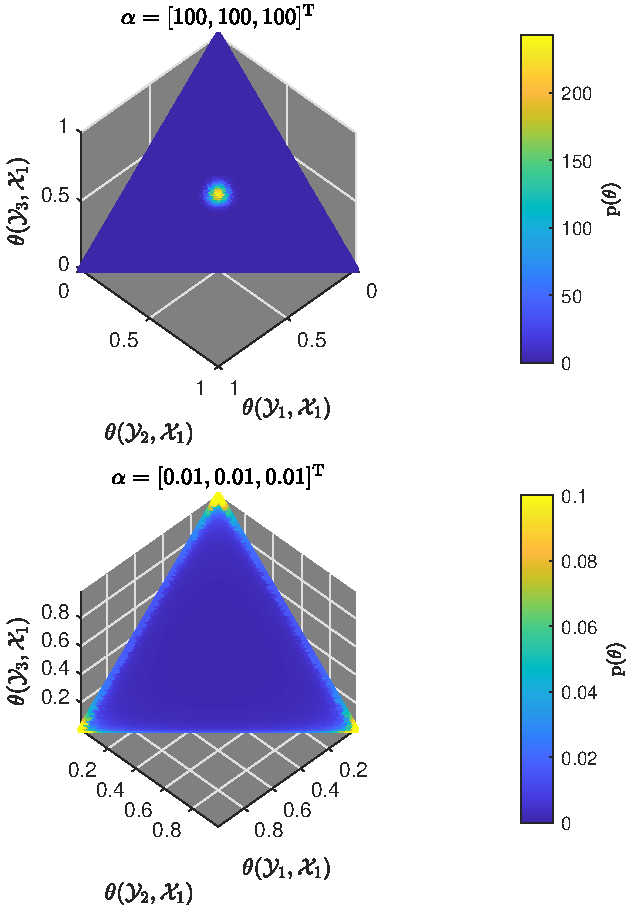
\includegraphics[width=0.7\linewidth]{P_theta.pdf}
\caption{Model prior PDF for different concentrations $\alpha_0$}
\label{fig:P_theta}
\end{figure}





\subsubsection{Uniform Prior}

When the parameterizing function is $\alpha(y,x) = 1$, the distribution becomes a uniform PDF and is represented as
\begin{equation}
\prm_{\uptheta} = \big( |\Ycal||\Xcal|-1 \big)! \;.
\end{equation}
Note that the concentration parameter is $\alpha_0 = |\Ycal||\Xcal|$ and $\Prm_{\yrm,\xrm} = \big( |\Ycal||\Xcal| \big)^{-1}$ is also uniform. 



\subsubsection{Marginal and Conditional Distributions}

The marginal distribution $\uptheta'$ and the conditional distribution $\tilde{\uptheta}$ will also be of interest. By the aggregation property \cite{ferguson}, $\uptheta'$ is a Dirichlet random process parameterized by $\alpha' : \Xcal \mapsto \Rbb^+$, where $\alpha' \equiv \sum_{y \in \Ycal} \alpha(y,\cdot)$. Note that $\Prm_{\xrm} = \mu_{\uptheta'} = \alpha' / \alpha_0$.


Also of interest is the distribution of the predictive model $\tilde{\uptheta}$ conditioned on the marginal $\uptheta'$. As demonstrated in Appendix \ref{app:Dir_agg}, these random processes are jointly distributed as
\begin{IEEEeqnarray}{rCl}
\prm_{\tilde{\uptheta} | \uptheta'}\Big( \tilde{\theta} | \theta' \Big) & = & \prod_{x \in \Xcal} \Bigg[ \beta\big( \alpha(\cdot,x) \big)^{-1} \prod_{y \in \Ycal} \tilde{\theta}(y;x)^{\alpha(y,x)-1} \Bigg] \\
& = & \prod_{x \in \Xcal} \Dir\Big( \tilde{\theta}(x) ; \alpha(\cdot,x) \Big) \nonumber \;,
\end{IEEEeqnarray}
a product of Dirichlet distributions defined on $\tilde{\theta} \in \Pcal(\Ycal)^{\Xcal}$. As shown, the processes $\tilde{\uptheta}(x)$ are Dirichlet with parameterizing functions $\alpha(\cdot,x)$, independent of one another, and independent of the marginal distribution $\uptheta'$. Observe that the values $\alpha'(x)$ represent the concentration parameters for the individual Dirichlet processes; also, note that $\Prm_{\yrm | \xrm} = \mu_{\tilde{\uptheta}(\xrm)} = \alpha(\cdot,\xrm) / \alpha'(\xrm)$. 


\begin{figure}
\centering
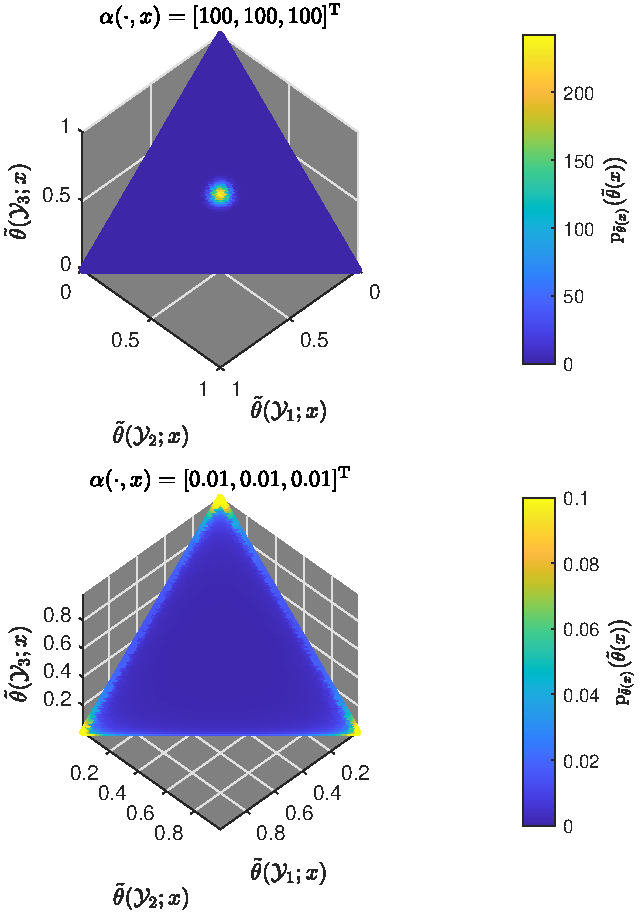
\includegraphics[width=0.7\linewidth]{P_theta_tilde.pdf}
\caption{Model prior PDF for different concentrations $\alpha'(x)$}
%\label{fig:P_theta}
\end{figure}












\subsection{Limited Support Priors}

Analyses will also be performed for decision functions derived from a variety of priors with limited-dimensional support. The implications of a degenerate prior probability distribution will be explored, with focus on limited training data volume benefits and issues. The asymptotic risk achieved by such learners will be of specific interest as well; while full support priors guarantee asymptotically consistent estimation of the true data-generating model, degenerate priors cannot ensure that the model is identified. 

Investigation into Bayesian learning with low-dimensional priors will have a special focus on applicability to human recognition tasks. In consideration of the insights into human recognition discussed in Section \ref{sec:prob}, special priors will be defined to reflect our own capabilities. 

The first motivating insight is that the data processed during human recognition is highly structured and seems to have an \emph{intrinsic dimensionality} that is much lower than that of the full dimensional space that they reside in. With this in mind, a potential restriction of the model support is
\begin{equation}
\big\| \theta' \big\|_0 = \sum_{x \in \Xcal} \Big(1 - \delta[\theta'(x),0] \Big) \leq M_{\Xcal} < |\Xcal| \;,
\end{equation}
which only considers marginal models with restricted $\ell_0$ norms. Figure \ref{fig:P_theta_limited_obs} shows how such a restriction for $|\Xcal| = 3$ lowers the intrinsic dimensionality of the prior support from 2-dimensional to 1-dimensional. Note that fewer parameters are needed to describe points in this subspace relative to a full support prior.
\begin{figure}
\centering
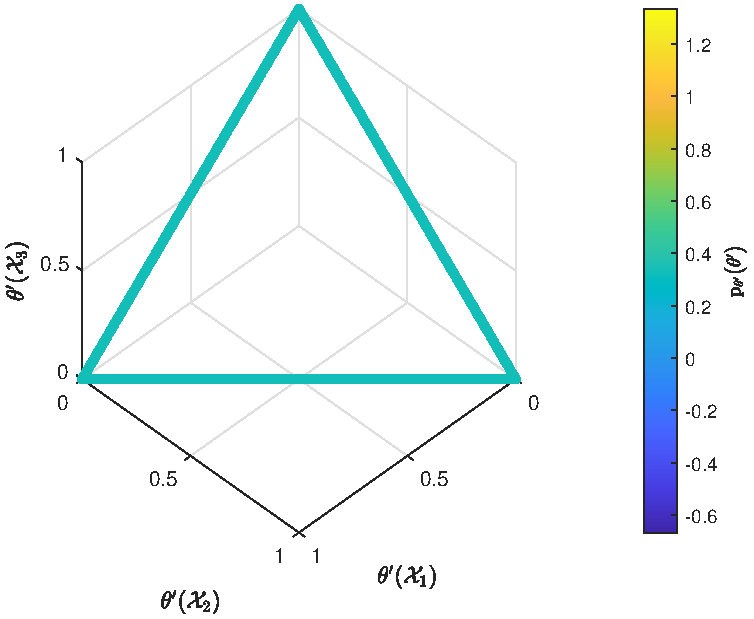
\includegraphics[width=0.6\linewidth]{P_theta_limited_obs.pdf}
\caption{Marginal model prior for $\big\| \theta' \big\|_0 \leq 2$}
\label{fig:P_theta_limited_obs}
\end{figure}

The second insight into human recognition is that our internal ``pre-processing'' greatly reduces the complexity of our sensory input. As such, machine learning functions should be able to perform feature extraction and effect significant dimensionality reduction without any loss of performance. This suggests that the prior distribution's support should be limited to a subspace that guarantees a low-dimensional \emph{sufficient statistic}.

To this effect, consider a transform function $T: \Xcal \mapsto \Tcal$ which maps to a lower-cardinality range $|\Tcal| \leq M_{\Xcal} < |\Xcal|$. The general function can be defined via its partitioning of the domain $\Xcal$ using the group of sets 
\begin{equation}
\Xcal_{\srm}(t) = \big\{ x \in \Xcal : T(x) = t \big\} \;, \quad t \in \Tcal \;,
\end{equation}
satisfying $\Xcal = \bigcup_{t \in \Tcal} \Xcal_{\srm}(t)$. 

Defining the transformed data random element $\trm \equiv T(\xrm)$, it can be shown that observation of the transform value refines the conditional data PMF as
\begin{equation}
\Prm_{\xrm | \uptheta',\trm}(x | \theta',t) = \frac{\theta'(x)}{\sum_{x' \in \Xcal_{\srm}(t)} \theta'(x')} \;,
\end{equation}
that is, the distribution $\Prm_{\xrm | \uptheta'}= \uptheta'$ normalized over the restricted domain defined by $T(x) = t$. 

For the transformed element to be a sufficient statistic, it must preserve all the original information from the observed data for inferences regarding $\uptheta'$. Formally, the requirement is that the obervation $\xrm$ is conditionally independent of the model $\uptheta'$ given the statistic $\trm$ \cite{kay-est}, which for this framework implies 
\begin{equation}
\frac{\theta'(x)}{\sum_{x' \in \Xcal_{\srm}(t)} \theta'(x')} = g(x;t) \;, \quad \forall x \in \Xcal, \; t \in \Tcal \;.
\end{equation}

Each of these conditions imposes a contraint on the set of models $\theta'$, lowering the dimensionality of the space on which any prior distribution may be defined. For example, consider the case $|\Xcal| = 3$ and $|\Tcal| = 2$; Figure \ref{fig:P_theta_suff_stat} illustrates a limited support prior distribution that would satisfy the requirements for such a sufficient statistic. 
\begin{figure}
\centering
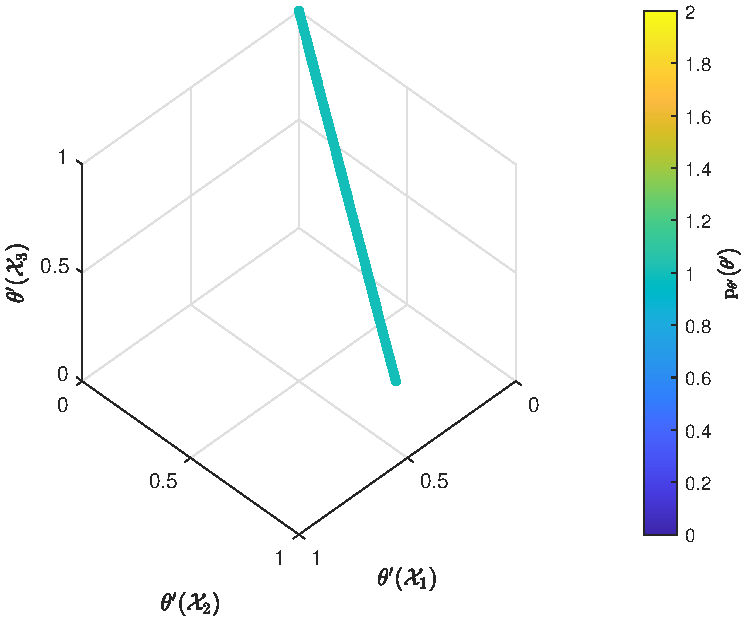
\includegraphics[width=0.6\linewidth]{P_theta_suff_stat.pdf}
\caption{A marginal model prior for $|\Tcal| = 2$}
\label{fig:P_theta_suff_stat}
\end{figure}
This demonstrates that in Bayesian learning, limited dimensional prior distributions can lead to the existence of data sufficient statistics. Further more, the degree of information compression provided by the statistic is inherently linked to the dimensionality of the prior's support. As such, the thesis will use limited-support prior distributions to form Bayesian predictive distributions that are suitable for human recognition applications. A primary research focus will be on how the user's intuition of sensible transformations $T$ drives the selection of the prior distribution support.



Another insight into human recognition performance is that we ourselves have defined the labels and their statistical relationship to our sensory observations, creating a joint distribution that leads to low clairvoyant risk. Casting this intuition into the learning framework used for this thesis, it is expected that the true predictive models $\tilde{\theta}(x)$ will be highly definitive, or in a sense, ``sparse''. Different metrics will be used to assess how certain a predictive model is. An obvious measure from information theory is conditional entropy (Figure \ref{fig:theta_tilde_entropy}), which could be restricted to low values. 
\begin{figure}
\centering
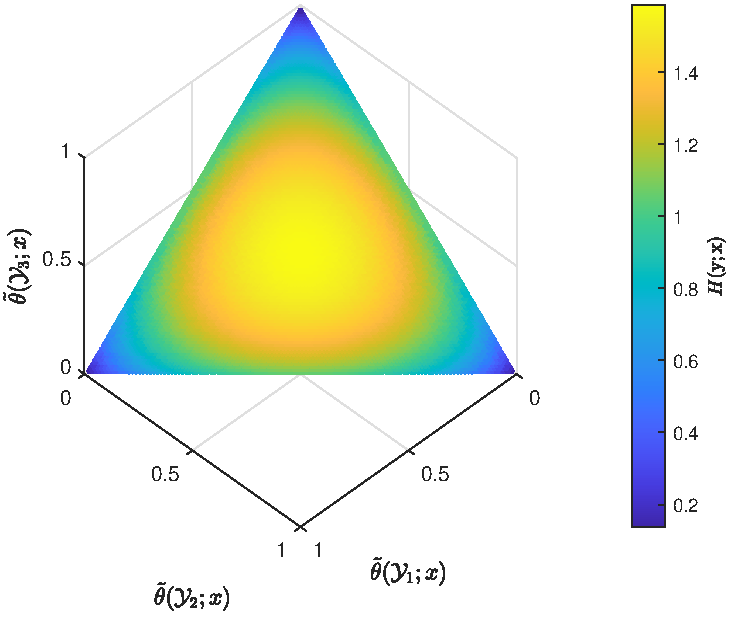
\includegraphics[width=0.6\linewidth]{theta_tilde_entropy.pdf}
\caption{Conditional entropy for $\tilde{\theta}(x)$}
\label{fig:theta_tilde_entropy}
\end{figure}
Another class of possible metrics are the $L^p$-norms. Of particular interest is the $L^{\infty}$ norm, $\big\| \tilde{\theta}(x) \big\|_{\infty} = \max_{y \in \Ycal} \big| \tilde{\theta}(y;x) \big|$, as it is equivalent to the 0--1 clairvoyant risk after an affine transformation. By providing a lower bound $\big\| \tilde{\theta}(x) \big\|_{\infty} \geq \rho > 1/|\Ycal|$ on the $L^{\infty}$ norms allowed, the prior support can be limited.
\begin{figure}
\centering
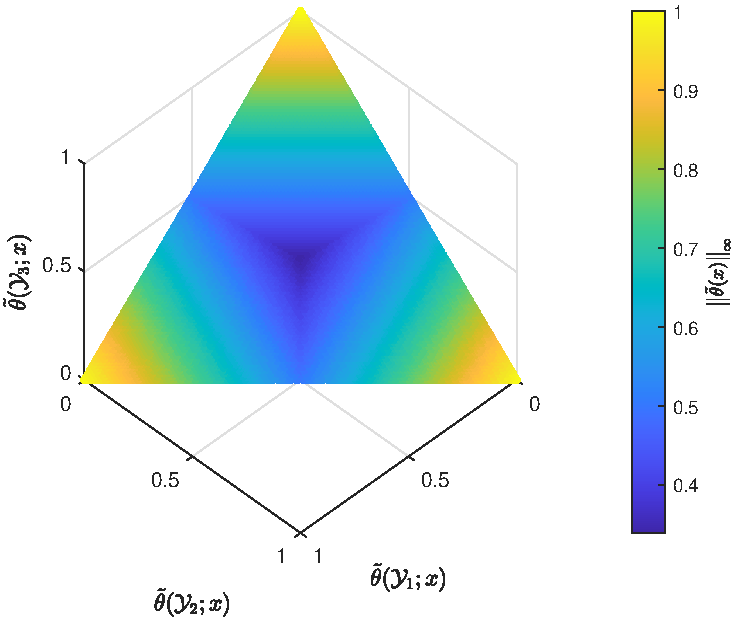
\includegraphics[width=0.6\linewidth]{theta_tilde_Linf.pdf}
\caption{$L^{\infty}$-norm of $\tilde{\theta}(x)$}
\label{fig:theta_tilde_Linf}
\end{figure}
While this restriction does limit the prior's support, it doesn't lower its dimensionality. With this in mind, another restriction that may be used is an upper bound on the $L^0$-norm, such that
\begin{equation}
\big\| \tilde{\theta}(x) \big\|_0  = \sum_{y \in \Ycal} \Big(1 - \delta\big[ \tilde{\theta}(y;x),0 \big] \Big) \leq M_{\Ycal} < |\Ycal| \;.
\end{equation}

If a sufficiently low value of $M_{\Ycal}$ is used, this condition alone may suffice; if it is used in conjunction with the $L^{\infty}$ condition, the intrinsic dimensionality of the prior support can be kept arbitrarily low while ensuring only models mapping to low clairvoyant risk are considered. Figure \ref{fig:theta_tilde_L0-inf} shows a possible restriction.
\begin{figure}
\centering
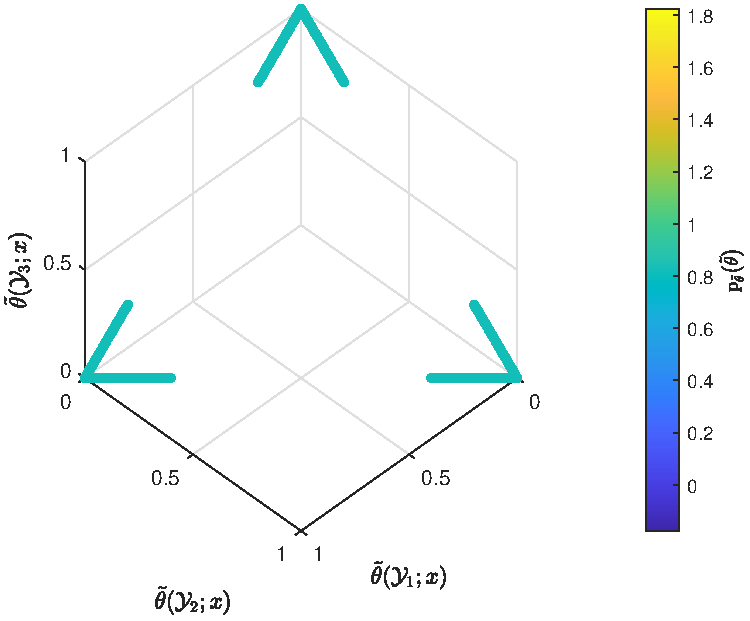
\includegraphics[width=0.6\linewidth]{theta_tilde_L0-inf.pdf}
\caption{Limited support for $\tilde{\theta}(x)$, $\big\| \tilde{\theta}(x) \big\|_0 \leq 2$, $\big\| \tilde{\theta}(x) \big\|_{\infty} \geq 0.8$}
\label{fig:theta_tilde_L0-inf}
\end{figure}

The most extreme restriction of this type would be to limit the predictive model $\tilde{\uptheta}(x)$ prior support to the $|\Ycal|$ PMF's satisfying $\big\| \tilde{\theta}(x) \big\|_{\infty} = 1$. By limiting the support to a countable set, the computational complexity of implementing decision functions based on such a prior will be minimized. While such functions have the potential to operate effectively on simpler problems, they will also undoubtedly be subject to the lack of adaptability inherent to learners based on extremely informative prior distributions. 













\section{Preliminary Results} \label{sec:results}

The work to date has focused on providing optimal decision functions and the resultant risk values when using Dirichlet prior distributions. Analysis of Bayesian estimators and classifiers for regression and classification, respectively, has been performed. Results accepted for publication include \emph{Predictive Distribution Estimation for Bayesian Machine Learning using a Dirichlet Prior}, presented at the 53rd Annual Asilomar Conference on Signals, Systems, and Computers and \emph{Bayesian Learning for Classification using a Uniform Dirichlet Prior}, presented at the 7th IEEE Global Conference on Signal and Information Processing.


This section details optimal decision functions when the sets $\Ycal$ and $\Xcal$ have a finite number of elements and the model $\uptheta$ is characterized by a Dirichlet distribution. The data marginal distribution $\Prm_{\nbarrm}$ and the Bayesian predictive PMF $\Prm_{\yrm | \xrm,\nbarrm}$ are provided and used for regression and classification applications via the squared-error and 0--1 loss functions, respectively.


\subsection{Probability Distributions}


\subsubsection{Training Set PMF, $\Prm_{\nbarrm}$}

Next, the distribution of the sufficient statistic $\nbarrm$ will be represented. As a Dirichlet distribution characterizes the parameters of the multinomial distribution $\Prm_{\Drm | \uptheta}$, the marginal PMF of $\nbarrm$ is a Dirichlet-Multinomial distribution \cite{johnson} parameterized by $\alpha$,
\begin{IEEEeqnarray}{rCl}
\Prm_{\nbarrm}(\bar{n}) & = & \Mcal(\bar{n}) \beta(\alpha)^{-1} \beta(\alpha + \bar{n}) \;.
\end{IEEEeqnarray}

The first and second joint moments of $\bar{\nrm}$ are
\begin{IEEEeqnarray}{rCl}
\mu_{\bar{\nrm}} & = & N \frac{\alpha}{\alpha_0} = N \mu_\uptheta 
\end{IEEEeqnarray}
and
\begin{IEEEeqnarray}{L}
\Erm_{\nbarrm}\big[ \bar{\nrm}(y,x) \bar{\nrm}(y',x') \big] \\
\qquad = \frac{N}{\alpha_0+1} \Big( (\alpha_0+N) \mu_\uptheta(y,x) \delta[y,y'] \delta[x,x'] + \alpha_0(N-1) \mu_\uptheta(y,x) \mu_\uptheta(y',x') \Big) \nonumber \;.
\end{IEEEeqnarray}
The covariance function is
\begin{IEEEeqnarray}{rCl}
\Sigma_{\nbarrm}(y,x,y',x') & = & \frac{N (\alpha_0+N)}{\alpha_0+1} \big( \mu_\uptheta(y,x) \delta[y,y'] \delta[x,x'] - \mu_\uptheta(y,x) \mu_\uptheta(y',x') \big) \\
& = & N (\alpha_0+N) \Sigma_{\uptheta}(y,x,y',x') \nonumber \;.
\end{IEEEeqnarray}


Again, the data PMF's for minimal and maximal concentration $\alpha_0$ are relevant. For $\alpha_0 \to \infty$, the model PDF $\prm_{\uptheta}$ concentrates at its mean and thus $\bar{\nrm}$ is characterized by a multinomial distribution,
\begin{IEEEeqnarray}{rCl}
\Prm_{\nbarrm}(\bar{n}) & \to & \Mcal(\bar{n}) \prod_{y \in \Ycal} \prod_{x \in \Xcal} \left(\frac{\alpha(y,x)}{\alpha_0}\right)^{\bar{n}(y,x)}
\end{IEEEeqnarray}
Conversely, for $\alpha_0 \to 0$, the PMF tends toward
\begin{IEEEeqnarray}{rCl} \label{eq:P_n_lim_zero}
\Prm_{\nbarrm}(\bar{n}) & \to & \sum_{y \in \Ycal} \sum_{x \in \Xcal} \frac{\alpha(y,x)}{\alpha_0} \delta\big[ \bar{n} , N \delta[\cdot,y] \delta[\cdot,x] \big] \;.
\end{IEEEeqnarray}

Figure \ref{fig:P_nbar_a0} displays the distribution of $\nbarrm$ for $N=10$ and different model concentrations $\alpha_0$. Observe that for large $\alpha_0$, the distribution approaches a multinomial distribution $\nbarrm \sim \Multi(N,\alpha/\alpha_0)$. Figure \ref{fig:P_nbar_N} shows how a specific model prior influences the data PMF differently for different $N$. Observe that as the number of training samples increases, the PMF $\Prm_{\nbarrm}$ tends toward $\Prm_{\nbarrm}(\bar{n}) \approx N^{1-|\Ycal||\Xcal|}\prm_{\uptheta}(\bar{n}/N)$; this can be proven using Gautschi's inequality \cite{wendel}.
\begin{figure}
\centering
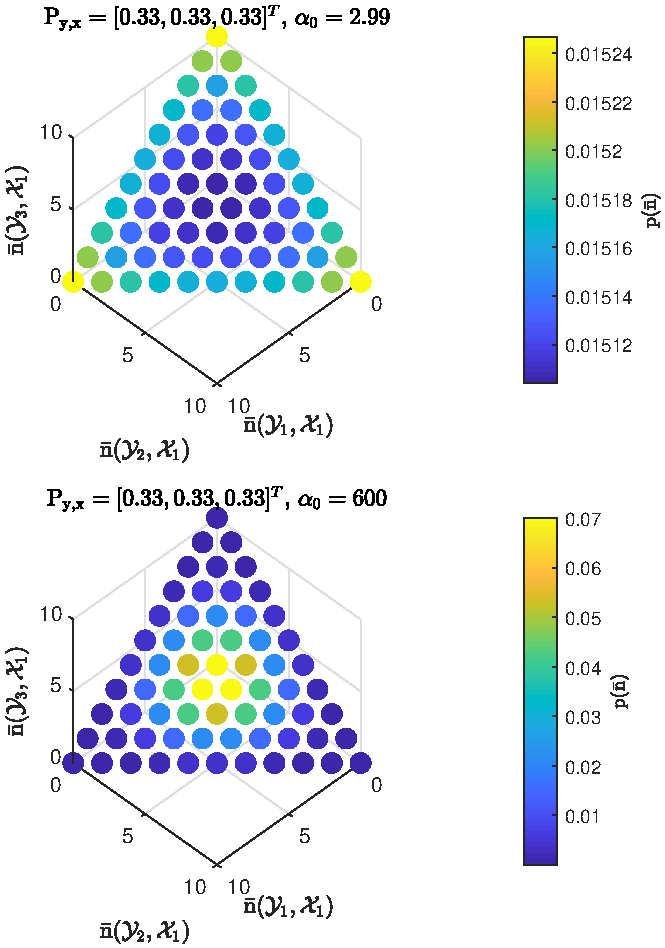
\includegraphics[width=0.7\linewidth]{P_nbar_a0.pdf}
\caption{$\Prm(\nbarrm)$ for different prior concentrations $\alpha_0$}
\label{fig:P_nbar_a0}
\end{figure}
\begin{figure}
\centering
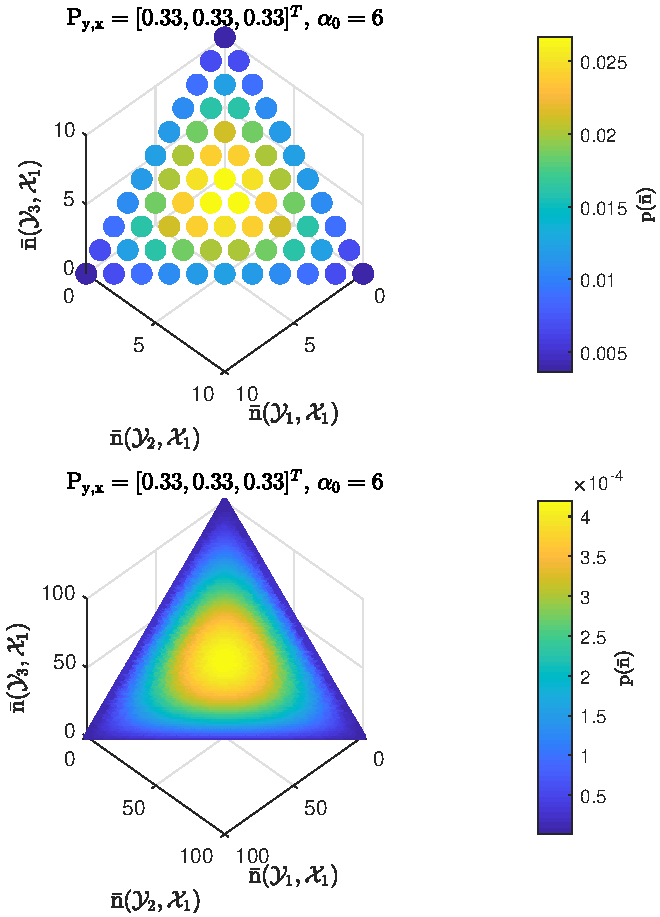
\includegraphics[width=0.7\linewidth]{P_nbar_N.pdf}
\caption{$\Prm(\nbarrm)$ for different training set sizes $N$}
\label{fig:P_nbar_N}
\end{figure}




\subparagraph{Uniform Prior}

For the uniform distribution, $\alpha(y,x) = 1$,
\begin{IEEEeqnarray}{rCl} \label{P_D_io}
\Prm_{\nbarrm} & = & |\bar{\Ncal}|^{-1} = \Mcal\big( \{N,|\Ycal||\Xcal|-1\} \big)^{-1} \;.
\end{IEEEeqnarray}
The distribution of $\nbarrm$ is uniform over the set $\bar{\Ncal}$. 





\paragraph{Marginal and Conditional Distributions}

It is also useful to express the marginal and conditional distributions for the training data given the Dirichlet prior. Recall that $\nrm' | \uptheta \sim \Multi(N,\uptheta')$; by the aggregation property of Dirichlet-Multinomial functions \cite{johnson}, the random process is distributed as $\nrm' \sim \DM(N,\alpha')$.

Also of interest is the distribution of $\nbarrm$ conditioned on its aggregation $\nrm'$. Using the Dirichlet-Multinomial properties presented in Appendix \ref{app:DM_agg}, it can be shown that
\begin{IEEEeqnarray}{rCl}
\Prm_{\bar{\nrm} | \nrm'}(\bar{n} | n') & = & \prod_{x \in \Xcal} \left[ \Mcal\big( \bar{n}(\cdot,x) \big) \beta\big( \alpha(\cdot,x) \big)^{-1} \beta\big( \alpha(\cdot,x) + \bar{n}(\cdot,x) \big) \right] \\
& = & \prod_{x \in \Xcal} \DM\Big( \bar{n}(\cdot,x) ; n'(x) , \alpha(\cdot,x) \Big) \nonumber
\end{IEEEeqnarray}
over the domain $\left\{ \bar{n} \in {\Zbb_{\geq 0}}^{\Ycal \times \Xcal} : \sum_{y \in \Ycal} \bar{n}(y,\cdot) = n' \right\}$. Observe that conditioning on the aggregation renders the function segments $\nbarrm(\cdot,x)$ independent of one another and that they are also Dirichlet-Multinomial, such that $\nbarrm(\cdot,x) | \nrm'(x) \sim \DM\big( \nrm'(x),\alpha(\cdot,x) \big)$.












\subsubsection{Predictive PMF, $\Prm_{\yrm | \xrm,\nbarrm}$}

As shown in Equation \eqref{eq:f_opt_xD}, the decision selected by the optimally designed function depends on $\Prm_{\yrm | \xrm,\nbarrm}$, the distribution of the unobserved $\yrm$ conditioned on all observable random elements. This PMF will be expressed next.


The Bayesian distributions $\Prm_{\xrm | \nbarrm}$ and $\Prm_{\yrm | \xrm,\nbarrm}$ can also be found from the posterior distributions $\prm_{\uptheta' | \nbarrm}$ and $\prm_{\tilde{\uptheta} | \xrm,\nbarrm}$, respectively. As the Dirichlet assumption renders $\uptheta'$ and $\tilde{\uptheta}$ independent, it can be shown that $\uptheta'$ is conditionally independent of $\nbarrm$ given $\nrm'$. Furthermore, the Dirichlet distribution $\prm_{\uptheta'}$ is the conjugate prior for $\Prm_{\nrm' | \uptheta'}$. As a result, $\uptheta' | \nrm' \sim \Dir(\alpha' + \nrm')$ and
\begin{IEEEeqnarray}{rCl}
\Prm_{\xrm | \nbarrm}(\bar{n}) & = & \mu_{\uptheta' | \nbarrm}(\bar{n}) = \mu_{\uptheta' | \nrm'}\left( \sum_y \bar{n}(y,\cdot) \right) \\
& = & \frac{\alpha' + \sum_y \bar{n}(y,\cdot)}{\alpha_0 + N} \nonumber \;,
\end{IEEEeqnarray}
where the dependency on $\nbarrm$ is expressed only through the marginal random process $\nrm'$.

The posterior $\prm_{\tilde{\uptheta} | \xrm,\nbarrm}$ can be simplified by noting that the independence of $\uptheta'$ and $\tilde{\uptheta}$ implies $\Prm_{\nbarrm | \nrm',\xrm} = \Erm_{\tilde{\uptheta}}\big[ \Prm_{\nbarrm | \nrm',\tilde{\uptheta}} \big] = \Prm_{\nbarrm | \nrm'}$. Consequently, $\tilde{\uptheta}$ is conditionally independent of $\xrm$ given $\nbarrm$. Thus, as $\prm_{\tilde{\uptheta}}$ is a conjugate prior for $\Prm_{\nbarrm | \nrm',\tilde{\uptheta}}$ the posterior distribution is
\begin{IEEEeqnarray}{rCl}
\prm_{\tilde{\uptheta} | \nbarrm,\xrm}\big( \tilde{\theta} | \bar{n},x \big) & = & \prm_{\tilde{\uptheta} | \nbarrm}\big( \tilde{\theta} | \bar{n} \big) = \prod_{x' \in \Xcal} \prm_{\tilde{\uptheta}(x') | \nbarrm(\cdot,x')}\big(\tilde{\theta}(x') | \bar{n}(\cdot,x') \big) \\
& = & \prod_{x' \in \Xcal} \Dir\big( \tilde{\theta}(x') ; \alpha(\cdot,x') + \bar{n}(\cdot,x') \big) \nonumber
\end{IEEEeqnarray}
and the distinct model conditional PMF's are independent from one another. Observe that when the conditioning is performed using the sufficient statistic, the independent conditional models $\tilde{\uptheta}(x)$ are only dependent on their corresponding subset of the empirical PMF, $\nbarrm(\cdot,x)$.



The concentration parameter for the predictive model posterior increases proportionately with increasing volumes of training data; consequently, as $n'(x) \to \infty$, the posterior converges to $\prm_{\tilde{\uptheta}(x) | \nbarrm} \to \delta\big( \cdot - \nbarrm(\cdot,x) / \nrm' \big)$. Thus, as more data is collected, the model can be more positively identified and used to formulate minimum risk decisions. Conversely, as $\alpha'(x) \to \infty$, the prior model certainty is stronger and the posterior tends toward $\prm_{\tilde{\uptheta}(x) | \nbarrm} \to \delta( \cdot - \alpha(\cdot,x) / \alpha'(x))$, independent of the training data.

Figure \ref{fig:P_theta_post_tilde} shows the influence of the training data on the model distribution; after conditioning on the training data (via $\nbarrm$), the PDF concentration shifts away from the models favored by the prior knowledge and towards other models that better account for the observations.
\begin{figure}
\centering
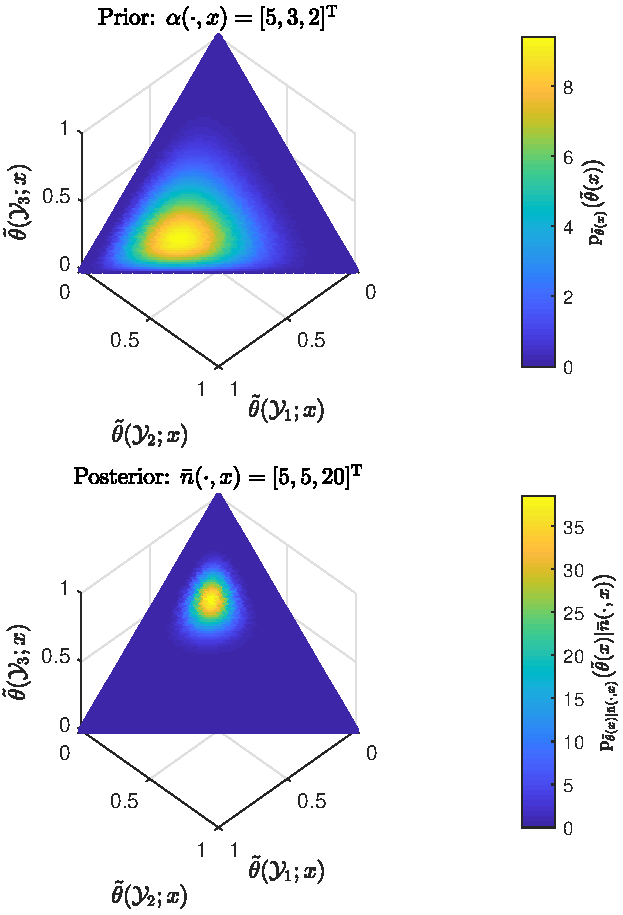
\includegraphics[width=0.7\linewidth]{P_theta_post_tilde.pdf}
\caption{Model PDF, prior and posterior}
\label{fig:P_theta_post_tilde}
\end{figure}




The Bayes predictive PMF can thus be expressed as
\begin{IEEEeqnarray}{rCl} \label{eq:P_y_xD_dir}
\Prm_{\yrm | \xrm,\nbarrm}(x,\bar{n}) & = & \mu_{\tilde{\uptheta}(x) | \xrm,\nbarrm}(x,\bar{n}) = \mu_{\tilde{\uptheta}(x) | \nbarrm(\cdot,x)}\big(\bar{n}(\cdot,x)\big) \\
& \equiv & \frac{\alpha(\cdot,x) + \bar{n}(\cdot,x)}{\alpha'(x) + n'(x)} \nonumber \\
& = & \left(\frac{\alpha'(x)}{\alpha'(x) + n'(x)}\right) \frac{\alpha(\cdot,x)}{\alpha'(x)} + \left(\frac{n'(x)}{\alpha'(x) + n'(x)}\right) \frac{\bar{n}(\cdot,x)}{n'(x)} \nonumber \;.
\end{IEEEeqnarray}
A consequence of the Dirichlet prior is that the predictive PMF for a given value of $\xrm$ only depends on the corresponding training data $\nbarrm(\cdot,\xrm)$, such that $\Prm_{\yrm | \xrm,\nbarrm}(x,\bar{n}) = \Prm_{\yrm | \xrm,\nbarrm(\cdot,\xrm)}\big( x,\bar{n}(\cdot,x) \big)$. This is intuitive considering the independence of the conditional models $\tilde{\theta}(x)$ from one another.

The last representation provided for $\Prm_{\yrm | \xrm,\nbarrm}$ interprets the distribution as a convex combination of two conditional distributions. The first distribution $\Prm_{\yrm | \xrm} = \alpha(\cdot,\xrm) / \alpha'(\xrm)$ is independent of the training data and based on the prior knowledge implied via the model PDF parameter; the second distribution is the conditional empirical PMF and depends only on the data

The weighting factors $\alpha'(x)$ and $n'(x)$ are the concentration of the conditional prior $\tilde{\uptheta}(x)$ and the number of training samples satisfying $X_n = \xrm$. As $n'(x) / \alpha'(x) \to 0$, the PMF tends toward the conditional distribution $\Prm_{\yrm | \xrm}$, which only depends on the model parameter $\alpha$. As $n'(x) / \alpha'(x) \to \infty$, $\Prm_{\yrm | \xrm,\nbarrm}$ tends towards the empirical conditional distribution.




\paragraph{Density Estimation Perspective} \label{sec:predictive_est}

It is informative to treat the distribution $\Prm_{\yrm | \xrm,\nbarrm}$ as an estimate of the unknown conditional PMF $\Prm_{\yrm | \xrm,\uptheta} \equiv \tilde{\uptheta}(\xrm)$ and investigate the effects of informative prior knowledge. For a given $\xrm$ and corresponding number of training samples $\nrm'(\xrm)$, the expected value of the estimate condtioned on the true model $\uptheta$ is
\begin{IEEEeqnarray}{L}
\Erm_{\nbarrm | \nrm',\uptheta}\big[ \Prm_{\yrm | \xrm,\nbarrm} \big] 
= \Erm_{\nbarrm(\cdot,\xrm) | \nrm'(\xrm),\tilde{\uptheta}(\xrm)}\big[ \Prm_{\yrm | \xrm,\nbarrm(\cdot,\xrm)} \big] \\ 
\quad = \left(\frac{\alpha'(\xrm)}{\alpha'(\xrm) + \nrm'(\xrm)}\right) \frac{\alpha(\cdot,\xrm)}{\alpha'(\xrm)} + \left(\frac{\nrm'(\xrm)}{\alpha'(\xrm) + \nrm'(\xrm)}\right) \tilde{\uptheta}(\xrm) \nonumber \;,
\end{IEEEeqnarray}
where the properties of a multinomial distribution conditioned on its aggregation have been used. The result is a convex combination of the conditional data-independent distribution $\alpha(\cdot,x) / \alpha'(x)$ and the true conditional distribution $\tilde{\uptheta}(\xrm)$. The convex coefficients are dependent on the ``marginal'' values $\alpha'$ and $\nrm'$; note that as the number of matching training samples $\nrm'(x)$ increases relative to $\alpha'(x)$, the estimate tends towards the true conditional PMF. 

To aid characterization of the estimator, define the random process $\Delta(\xrm,\nbarrm,\uptheta) \equiv \Prm_{\yrm | \xrm,\nbarrm} - \Prm_{\yrm | \xrm,\uptheta} \in \Rbb^{\Ycal}$. For a given $\xrm$ and corresponding number of training samples $\nrm'(\xrm)$, the bias of the conditional PMF estimate is
\begin{IEEEeqnarray}{rCl} \label{eq:predictive_bias}
\mathrm{Bias}(\xrm,\nrm',\uptheta) & = & \Erm_{\nbarrm | \nrm',\uptheta}\big[ \Delta(\xrm,\nbarrm,\uptheta) \big] \\
& = & \frac{\alpha'(\xrm)}{\alpha'(\xrm) + \nrm'(\xrm)} \left( \frac{\alpha(\cdot,\xrm)}{\alpha'(\xrm)} - \tilde{\uptheta}(\xrm) \right) \nonumber 
\end{IEEEeqnarray}
and its covariance function is 
\begin{IEEEeqnarray}{L} \label{eq:predictive_cov}
\mathrm{Cov}(y,y';\xrm,\nrm',\uptheta) = \Crm_{\nbarrm | \nrm',\uptheta} \big[\Prm_{\yrm | \xrm,\nbarrm}(\cdot | \xrm,\nbarrm) \big](y,y') \\
\quad = \frac{\Sigma_{\nbarrm(\cdot,\xrm) | \nrm'(\xrm),\tilde{\uptheta}(\xrm)}(y,y')}{\big( \alpha'(\xrm) + \nrm'(\xrm) \big)^2} \nonumber \\
\quad = \frac{\nrm'(\xrm)}{\big( \alpha'(\xrm) + \nrm'(\xrm) \big)^2} \left( \tilde{\uptheta}(y;\xrm) \delta[y,y'] - \tilde{\uptheta}(y;\xrm) \tilde{\uptheta}(y';\xrm) \right) \nonumber \;,
\end{IEEEeqnarray}
where the properties of multinomial random processes have been used. Note that the bias is proportionate to the difference between the true conditional model and the data-independent estimate. The scaling factor tends from one to zero as $\nrm'(x)/\alpha'(x)$ tends from zero to infinity; as such, more informative priors (large $\alpha'(x)$) will lead to PMF estimates that are prone to bias. Conversely, the variance of the PMF estimate tends to zero as $\alpha'(x) \to \infty$. 


Combining the estimator bias and variance, the conditional second moments of $\Delta(\xrm,\nbarrm,\uptheta)$ are
\begin{IEEEeqnarray}{rCl} \label{eq:predictive_del_sq}
\mathcal{E}(y,y' ; \xrm,\nrm',\uptheta) & = & \Erm_{\nbarrm | \nrm',\uptheta} \Big[ \Delta(y;\xrm,\nbarrm,\uptheta) \Delta(y';\xrm,\nbarrm,\uptheta) \Big] \\
& = & \mathrm{Bias}(y;\xrm,\nrm',\uptheta) \mathrm{Bias}(y';\xrm,\nrm',\uptheta) + \mathrm{Cov}(y,y';\xrm,\nrm',\uptheta) \nonumber \;.
\end{IEEEeqnarray}
As $\nrm'(x) \to \infty$, this function tends to zero and thus the underlying model $\tilde{\uptheta}(x)$ is determined precisely. A more practical case is estimation with a finite volume of training data. Specification of the Dirichlet model prior can be interpreted as providing a distribution estimate $\alpha(\cdot,x)/\alpha'(x)$ and a confidence level $\alpha'(x)$. Higher confidence reduces error due to the variance of the estimator, but increases the error due to bias between the true model and its estimate; low confidence renders the estimate unbiased, but maximizes the estimator variance. 



Also of interest, the conditional expectation of $\mathcal{E}(\cdot,\cdot;\xrm,\nrm',\uptheta)$ is
\begin{IEEEeqnarray}{L} \label{eq:predictive_E_del_sq}
\Erm_{\xrm,\nrm' | \uptheta}\Big[ \mathcal{E}(y,y' ; \xrm,\nrm',\uptheta) \Big] \\
\quad = \Erm_{\xrm | \uptheta}\left[ \Erm_{\nrm'(\xrm) | \uptheta}\left[ \left(\frac{\alpha'(\xrm)}{\alpha'(\xrm) + \nrm'(\xrm)}\right)^2 \right] \left( \frac{\alpha(y,\xrm)}{\alpha'(\xrm)} - \tilde{\uptheta}(y;\xrm) \right) \left( \frac{\alpha(y',\xrm)}{\alpha'(\xrm)} - \tilde{\uptheta}(y';\xrm) \right) \right] \nonumber \\
\qquad + \Erm_{\xrm | \uptheta}\left[ \Erm_{\nrm'(\xrm) | \uptheta}\left[ \frac{\nrm'(\xrm)}{\big( \alpha'(\xrm) + \nrm'(\xrm) \big)^2} \right] \left( \tilde{\uptheta}(y;\xrm) \delta[y,y'] - \tilde{\uptheta}(y;\xrm) \tilde{\uptheta}(y';\xrm) \right) \right] \nonumber \;.
\end{IEEEeqnarray}



To exemplify how the model estimate $\Prm_{\yrm | \xrm,\nbarrm}$ approximates $\Prm_{\yrm | \xrm,\uptheta}$, consider a scenario with $|\Ycal| = 10$. The data-independent PMF $\alpha(\cdot,x) / \alpha'(x)$ and true model $\tilde{\uptheta}(x)$ are shown in Figure \ref{fig:P_yx_error_N_0} - note the significant mismatch. 

Figures \ref{fig:P_yx_error_a0_0_1} and \ref{fig:P_yx_error_a0_10} show how the bias and variance of the estimate change for different values of $\nrm'(x)$ and $\alpha'(x)$. The plot markers represent the conditional mean of the estimator, $\Erm_{\nbarrm | \nrm',\uptheta}\big[ \Prm_{\yrm | \xrm,\nbarrm}(y | \xrm,\nbarrm) \big]$; the upper and lower error bars represent the square-root of the expected squared deviation above and below the conditional mean, respectively. Each individual plot heading provides the error $\sqrt{\sum_{y \in \Ycal} \mathcal{E}(y,y ; \xrm,\nrm',\uptheta)}$ to assess the quality of the PMF estimate. 

Observe that for $\nrm'(x) = 1$, the high variance of the $\alpha'(x) = 0.1$ estimate (favoring the empirical PMF) renders it worse than the $\alpha_0 = 10$ estimate; in fact, the variance is so high that the error exceeds that of the data-independent estimate $\alpha(\cdot,x) / \alpha'(x)$ (Figure \ref{fig:P_yx_error_N_0}). Conversely, for $\nrm'(x) = 10$, the confidence of the $\alpha'(x) = 10$ estimate leads to high bias and the $\alpha'(x) = 0.1$ estimate is superior. For $\nrm'(x) = 100$, both the $\alpha'(x) = 0.1$ and $\alpha'(x) = 10$ estimates begin converging to the true distribution - this is guaranteed due to the full support of the Dirichlet prior.


\begin{figure}
\centering
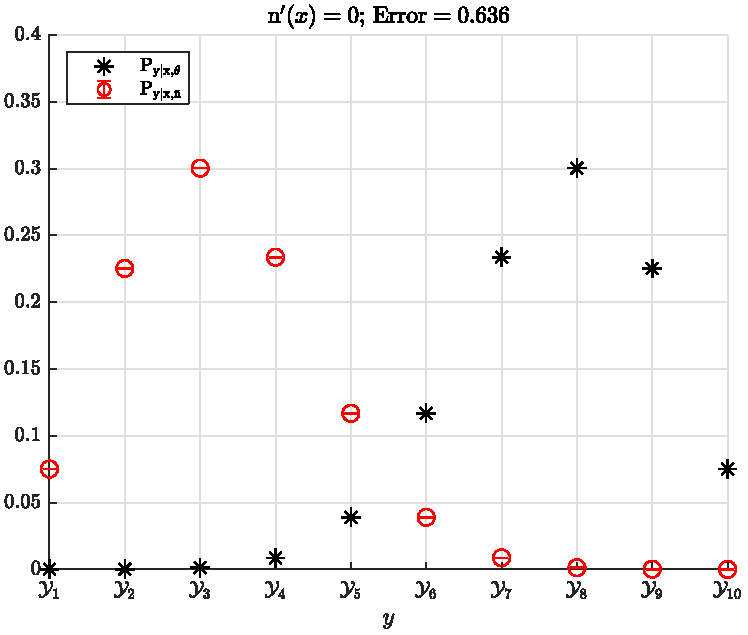
\includegraphics[width=0.7\linewidth]{P_yx_error_N_0.pdf}
\caption{Model $\uptheta$ estimate, no training data}
\label{fig:P_yx_error_N_0}
\end{figure}

\begin{figure}
\centering
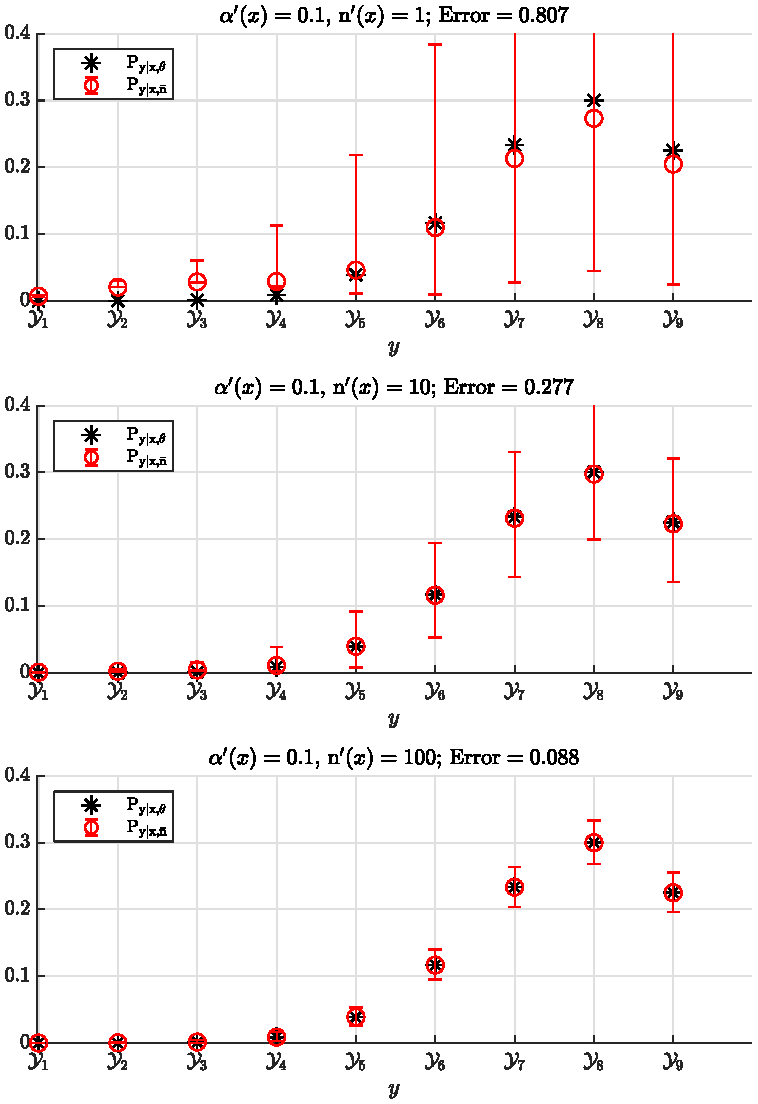
\includegraphics[width=0.7\linewidth]{P_yx_error_a0_0_1.pdf}
\caption{Model $\uptheta$ estimates, $\alpha_0 = 0.1$}
\label{fig:P_yx_error_a0_0_1}
\end{figure}

\begin{figure}
\centering
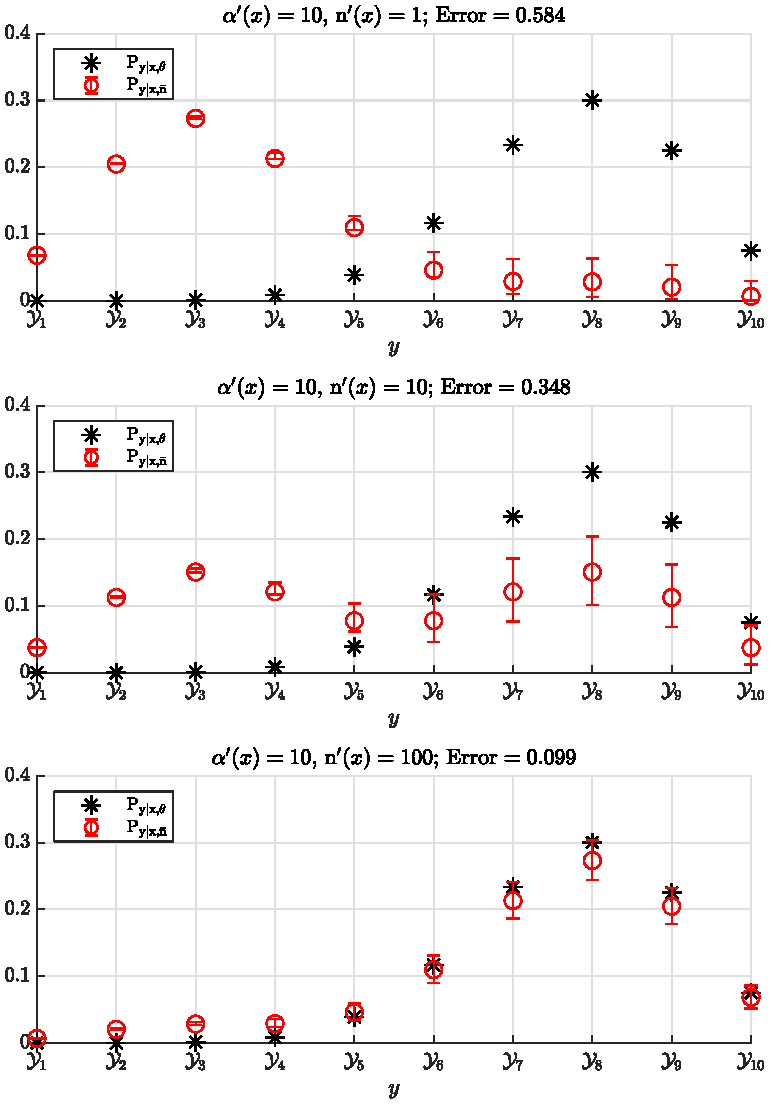
\includegraphics[width=0.7\linewidth]{P_yx_error_a0_10.pdf}
\caption{Model $\uptheta$ estimates, $\alpha_0 = 10$}
\label{fig:P_yx_error_a0_10}
\end{figure}
















\subsection{Applications to Common Loss Functions}

In this section, the Dirichlet prior is applied to the regression and classification applications. Optimal learners $f^*$ are found,  the corresponding minimum Bayes risk $\Rcal^*$ is assessed, and the conditional risk $\Rcal_{\Theta}(f^*;\theta)$ is analyzed.

It is informative to substitute the Bayes predictive distribution using the Dirichlet prior \eqref{eq:P_y_xD_dir} into Equation \eqref{eq:f_opt_xD}, expressing the decision for a given input $\xrm$ and training set $\Drm$ as
\begin{IEEEeqnarray}{L} \label{eq:E_y|xD L}
f^*(\xrm;\Drm) = \argmin_{h \in \Hcal} \Erm_{\yrm | \xrm,\Drm} \big[ \Lcal(h,\yrm) \big] \\
= \argmin_{h \in \Hcal} \left(\frac{\alpha'(\xrm)}{\alpha'(\xrm) + N'(\xrm;\Drm)}\right) \sum_{y \in \Ycal} \frac{\alpha(y,\xrm)}{\alpha'(\xrm)} \Lcal(h,y) + \left(\frac{N'(\xrm;\Drm)}{\alpha'(\xrm) + N'(\xrm;\Drm)}\right) \sum_{y \in \Ycal} \frac{\bar{N}(y,\xrm;\Drm)}{N} \Lcal(h,y) \nonumber \\
= \argmin_{h \in \Hcal} \left(\frac{\alpha'(\xrm)}{\alpha'(\xrm) + N'(\xrm;\Drm)}\right) \Erm_{\yrm | \xrm}\big[ \Lcal(h,\yrm) \big] + \left(\frac{N'(\xrm;\Drm)}{\alpha'(\xrm) + N'(\xrm;\Drm)}\right) \frac{\sum_{n=1}^N \delta\big[ \xrm,\Xrm_n \big] \Lcal\big( h,\Yrm_n \big)}{\sum_{n=1}^N \delta\big[ \xrm,\Xrm_n \big]} \nonumber \;.
\end{IEEEeqnarray}

The metric to be minimized can be represented as a convex combination of two expected losses. The first expected loss is evaluated with respect to the conditional distribution $\Prm_{\yrm | \xrm} = \alpha(\cdot,\xrm) / \alpha'(\xrm)$, which reflects the prior knowledge imparted by the model parameter $\alpha$. The second term is a conditional emprical loss, or the average loss among samples $\Yrm_n$ whose corresponding values $\Xrm_n$ match the observed value $\xrm$. The convex weights are inherited from the conditional distribution $\Prm_{\yrm | \xrm,\Drm}$; thus, for a given observation $\xrm$, the model prior parameter $\alpha'(\xrm)$ and the number of matching training samples $N'(\xrm;\Drm)$ dictate which of the two expectations are emphasized.




\subsubsection{Regression: the Squared-Error Loss}

The elements of the finite cardinality set $\Ycal$ are real numbers, such that $\Ycal \subset \Rbb$. Again, $\Hcal = \Rbb \supset \Ycal$.



\paragraph{Bayesian Estimation}

Substituting in the Bayes predictive distribution for a Dirichlet prior into \eqref{eq:f_opt_SE}, the optimal Bayesian estimate is
\begin{IEEEeqnarray}{rCl} \label{eq:f_opt_SE_dir}
f^*(\xrm;\Drm) & = & \mu_{\yrm | \xrm,\Drm} \\
& = & \left( \frac{\alpha'(\xrm)}{\alpha'(\xrm) + N'(\xrm;\Drm)} \right) \sum_{y \in \Ycal} y \frac{\alpha(y,\xrm)}{\alpha'(\xrm)} + \left( \frac{N'(\xrm;\Drm)}{\alpha'(\xrm) + N'(\xrm;\Drm)} \right) \sum_{y \in \Ycal} y \frac{\bar{N}(y,\xrm;\Drm)}{N'(\xrm;\Drm)} \nonumber \\
& = & \left( \frac{\alpha'(\xrm)}{\alpha'(\xrm) + N'(\xrm;\Drm)} \right) \mu_{\yrm | \xrm} + \left( \frac{N'(\xrm;\Drm)}{\alpha'(\xrm) + N'(\xrm;\Drm)} \right) \frac{\sum_{n=1}^N \delta\big[ \xrm,\Xrm_n \big] \Yrm_n}{N'(\xrm;\Drm)} \nonumber \;.
\end{IEEEeqnarray}

The optimal estimate is interpreted as a convex combination of two separate estimates - the expected value of $\yrm$ conditioned on the observed $\xrm$ and the mean of the training values $\Yrm_n$ which have a value $\Xrm_n$ matching the observed value $\xrm$. The weighting factors are the same as those of $\Prm_{\yrm | \xrm,\Drm}$; thus, stronger prior information (larger $\alpha'(\xrm)$) provides more weight to the estimate $\mu_{\yrm|\xrm}$ and more voluminous training data puts emphasis on the empirical conditional mean.




The minimum Bayes squared-error is $\Rcal^* = \Erm_{\xrm,\Drm} \left[ \Sigma_{\yrm | \xrm,\Drm} \right]$. Using the sufficient statistic $\nbarrm \equiv \bar{N}(\Drm)$, the minimum risk can also be represented as $\Erm_{\xrm,\nbarrm} \left[ \Sigma_{\yrm | \xrm,\nbarrm} \right]$; as such, the expectations are performed over $\nbarrm$. Decompose the conditional variance as
\begin{IEEEeqnarray}{rCl}
\Sigma_{\yrm | \xrm,\nbarrm} & = & \Erm_{\yrm | \xrm,\nbarrm}[\yrm^2] - \mu_{\yrm | \xrm,\nbarrm}^2 
\end{IEEEeqnarray}
and assess the expected values of these terms separately using distributions derived from the Dirichlet prior. The first term is simply
\begin{IEEEeqnarray}{rCl}
\Erm_{\xrm,\nbarrm} \left[ \Erm_{\yrm | \xrm,\nbarrm}[\yrm^2] \right] & = & \Erm_{\yrm}[\yrm^2] = \sum_{y \in \Ycal} y^2 \left( \sum_{x \in \Xcal} \frac{\alpha(y,x)}{\alpha_0} \right) \nonumber \\
& = & \Erm_{\xrm} \big[ \Erm_{\yrm | \xrm} [ \yrm^2 ] \big] = \sum_{x \in \Xcal} \frac{\alpha'(x)}{\alpha_0} \sum_{y \in \Ycal} y^2 \frac{\alpha(y,x)}{\alpha'(x)} \nonumber \;,
\end{IEEEeqnarray}
where the different functions of $\alpha$ are represented by the PMF's of $\yrm$ and $\xrm$. Next, find, 
\begin{IEEEeqnarray}{rCl}
\Erm_{\xrm,\nbarrm} \Big[ \mu_{\yrm | \xrm,\nbarrm}^2 \Big] & = & \Erm_{\xrm} \left[ \Erm_{\nbarrm | \xrm} \left[ \frac{\big( \alpha'(\xrm) \mu_{\yrm|\xrm} + \sum_{y \in \Ycal} y \bar{\nrm}(y,\xrm) \big)^2}{\alpha'(\xrm) \big(\alpha'(\xrm) + \nrm'(\xrm) \big)^2} \right] \right] \\
& = & \Erm_{\xrm} \left[ \Erm_{\nbarrm} \left[ \frac{\alpha_0 \big( \alpha'(\xrm) \mu_{\yrm|\xrm} + \sum_{y \in \Ycal} y \bar{\nrm}(y,\xrm) \big)^2}{\alpha'(\xrm) \big(\alpha'(\xrm) + \nrm'(\xrm) \big) (\alpha_0+N)} \right] \right] \nonumber \\
& = & \Erm_{\xrm} \left[ \Erm_{\nrm'} \left[ \frac{\alpha_0 \Erm_{\nbarrm | \nrm'} \left[ \big( \alpha'(\xrm) \mu_{\yrm|\xrm} + \sum_{y \in \Ycal} y \bar{\nrm}(y,\xrm) \big)^2 \right]}{\alpha'(\xrm) \big(\alpha'(\xrm) + \nrm'(\xrm) \big) (\alpha_0+N)} \right] \right] \nonumber \\
& = & \Erm_{\xrm} \left[ \frac{\alpha_0 \Erm_{\nrm'} \Big[ \nrm'(\xrm) \Erm_{\yrm|\xrm}[\yrm^2] + \big( \alpha'(\xrm) + \nrm'(\xrm) + 1 \big) \alpha'(\xrm) \mu_{\yrm|\xrm}^2 \Big]}{\alpha'(\xrm) \big(\alpha'(\xrm) + 1 \big) (\alpha_0+N)} \right] \nonumber \\
& = & \Erm_{\xrm} \left[ \frac{N \Erm_{\yrm|\xrm}[\yrm^2] + \big( \alpha_0 \alpha'(\xrm) + N \alpha'(\xrm) + \alpha_0 \big) \mu_{\yrm|\xrm}^2 }{\big( \alpha'(\xrm)+1 \big) (\alpha_0+N)} \right] \nonumber \;.
\end{IEEEeqnarray}

The above formulation exploits the statistical characterization of the aggregation, $\nrm' \sim \DM(N,\alpha')$; also used is the property that the Dirichlet-Multinomial random process $\nbarrm$ conditioned on its aggregation $\nrm'$ yields independent  conditional DM functions $\bar{\nrm}(\cdot,x) | \nrm'(x) \sim \DM\big( \nrm'(x),\alpha(\cdot,x) \big)$.

Finally, combine the two formulas to represent the mininum Bayes risk,
\begin{IEEEeqnarray}{L}
\Rcal^* = \Erm_{\xrm,\nbarrm} \left[ \Erm_{\yrm | \xrm,\nbarrm}[\yrm^2] - \mu_{\yrm | \xrm,\nbarrm}^2 \right] \\
= \Erm_{\xrm} \left[ \frac{\alpha_0 \alpha'(\xrm) + N \alpha'(\xrm) + \alpha_0}{\big( \alpha'(\xrm)+1 \big) (\alpha_0+N)} \Sigma_{\yrm | \xrm} \right] \nonumber \\
= \Erm_{\xrm} \left[ \frac{\Prm_{\xrm}(\xrm) + (\alpha_0+N)^{-1}}{\Prm_{\xrm}(\xrm) + \alpha_0^{-1}} \Sigma_{\yrm | \xrm} \right] \nonumber \;.
\end{IEEEeqnarray}
The minimum risk is the expected value of the scaled conditional variance with respect to $\Prm_{\yrm | \xrm} = \alpha(\cdot,\xrm)/\alpha'(\xrm)$. The expectation is taken with respect to the prior marginal distribution $\Prm_{\xrm} = \alpha'/\alpha_0$. 

The scaling factor for each term $\Sigma_{\yrm | \xrm}$ depends on the marginal $\Prm_{\xrm}$, as well as on the prior concentration $\alpha_0$ and the number of training samples $N$. Observe that with no training data ($N = 0$), the scaling factor becomes unity and the risk is $\Rcal^* = \Erm_{\xrm} \left[ \Sigma_{\yrm | \xrm} \right]$. Conversely, as $N \to \infty$, the Bayes risk is $\Rcal^* \to \Erm_{\xrm} \left[ \frac{\Prm_{\xrm}(\xrm)}{\Prm_{\xrm}(\xrm) + \alpha_0^{-1}} \Sigma_{\yrm | \xrm} \right]$; note that this is equivalent to the irreducible risk $\Erm_{\uptheta}\big[\Rcal_{\Theta}^*(\uptheta)\big] = \Erm_{\xrm,\uptheta} \left[ \Sigma_{\yrm | \xrm,\uptheta} \right]$. Also, as the model concentration parameter $\alpha_0 \to 0$, the risk tends to zero (for $N > 0$); as $\alpha_0 \to \infty$, the risk tends toward $\Erm_{\xrm} \left[ \Sigma_{\yrm | \xrm} \right]$.

To illustrate these trends, explicitly define the sets $\Ycal = \{ i/M_{\yrm} : i = 0,\ldots,M_{\yrm}-1 \}$ and $\Xcal = \{ i/M_{\xrm} : i = 0,\ldots,M_{\xrm}-1 \}$. Assume that the conditional variance $\Sigma_{\yrm | \xrm}$ is independent of $\xrm$; in this case, the squared-error becomes the conditional variance scaled by a factor dependent on the marginal distribution $\Prm(\xrm)$, such that $\Rcal^* = \Sigma_{\yrm | \xrm} \Erm_{\xrm} \left[ \frac{\Prm_{\xrm}(\xrm) + (\alpha_0+N)^{-1}}{\Prm_{\xrm}(\xrm) + \alpha_0^{-1}} \right]$.  Figures \ref{fig:Risk_SE_Dir_IO_N_leg_a0} and \ref{fig:Risk_SE_Dir_IO_a0_leg_N} display how the risk changes with $N$ and $\alpha_0$ when $\Prm_{\yrm | \xrm}$ and $\Prm_{\xrm}$ are fixed.

\begin{figure}
\centering
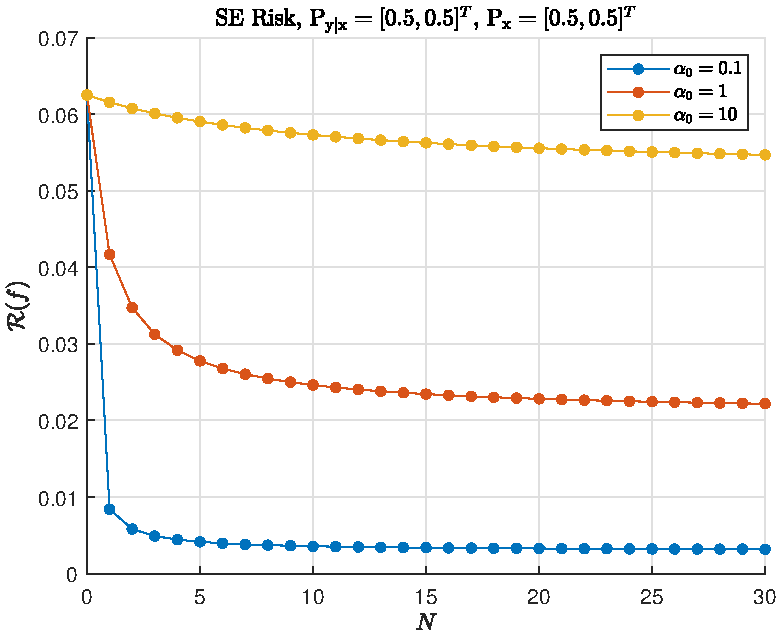
\includegraphics[width=0.7\linewidth]{Risk_SE_Dir_IO_N_leg_a0.pdf}
\caption{Minimum SE Risk for different training set sizes $N$}
\label{fig:Risk_SE_Dir_IO_N_leg_a0}
\end{figure}

\begin{figure}
\centering
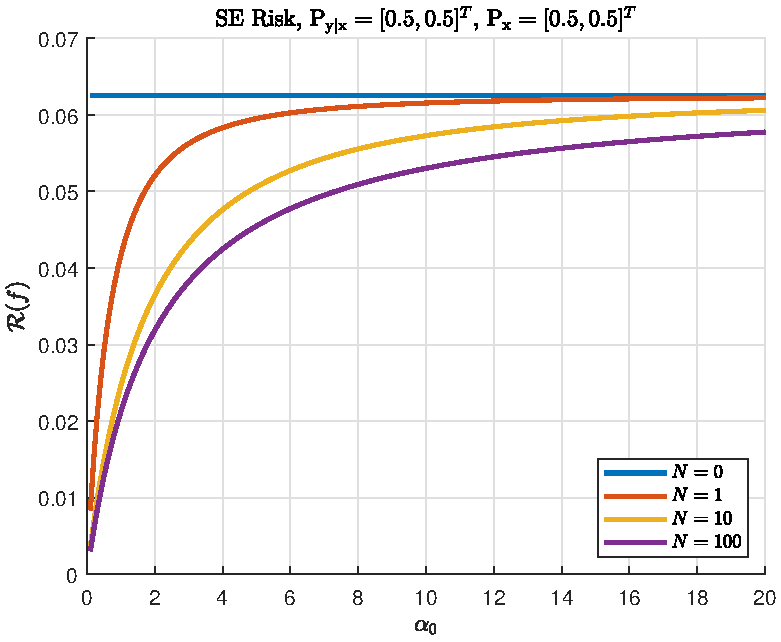
\includegraphics[width=0.7\linewidth]{Risk_SE_Dir_IO_a0_leg_N.pdf}
\caption{Minimum SE Risk for different prior concentrations $\alpha_0$}
\label{fig:Risk_SE_Dir_IO_a0_leg_N}
\end{figure}

It may not seem intutitve for the risk to decrease when $\alpha_0$ is smaller -- the variance of the model $\uptheta$ increases and the prior knowledge is less definitive. This is a result of the Dirichlet PDF weight shifting towards the $|\Ycal||\Xcal|$ models which have $\ell_0$ norms satisfying $\| \theta \|_0 = 1$. Although these PMF's are maximally separated (and uncorrelated), they all have zero variance. The optimal learner \eqref{eq:f_opt_SE_dir} will simply use the empirical distribution supplied via the training data - this allows exact identification of $\uptheta$ with a single training pair.

It is also informative to visualize how the minimum squared-error changes for fixed volume of training data $N$ and a fixed prior concentration $\alpha_0$. First, consider how the risk changes with the conditional PMF $\Prm_{\yrm | \xrm}$. Figure \ref{fig:Risk_SE_Dir_IO_Pyx} demonstrates how the squared-error tends towards zero for PMFs that have $\ell_0$-norm equal to one.
\begin{figure}
\centering
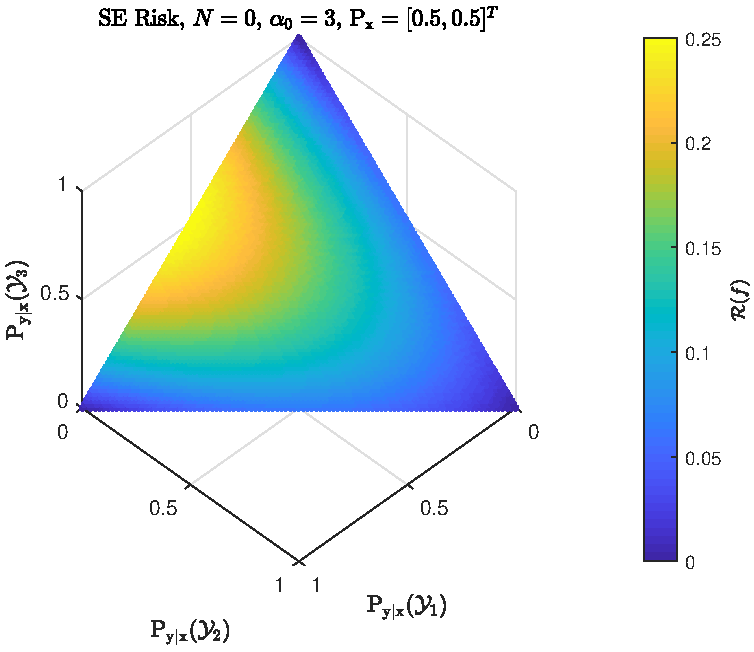
\includegraphics[width=0.7\linewidth]{Risk_SE_Dir_IO_Pyx.pdf}
\caption{Minimum SE Risk for different PMF's $\Prm(\yrm | \xrm)$}
\label{fig:Risk_SE_Dir_IO_Pyx}
\end{figure}

Next, consider the effect of the marginal distribution $\Prm_{\xrm}$. Figure \ref{fig:Risk_SE_Dir_IO_Px_N_10_a0_1} demonstrates how the risk changes with this marginal PMF. Observe that the risk is maximal at the distributions satisfying $\| \Prm_{\xrm} \|_0 = 1$; the scaling factor for the conditional variance $\Sigma_{\yrm | \xrm}$ becomes $\frac{1 + (\alpha_0+N)^{-1}}{1 + \alpha_0^{-1}}$. Conversely, for $\Prm_{\xrm} = 1/|\Xcal|$ the scaling factor becomes $\frac{|\Xcal|^{-1} + (\alpha_0+N)^{-1}}{|\Xcal|^{-1} + \alpha_0^{-1}}$ and the risk is minimal. Figures \ref{fig:Risk_SE_Dir_IO_N_leg_Px} and \ref{fig:Risk_SE_Dir_IO_a0_leg_Px} show how different marginals $\Prm_{\xrm}$ affect the risk as a function of $N$ and $\alpha_0$, respectively.

\begin{figure}
\centering
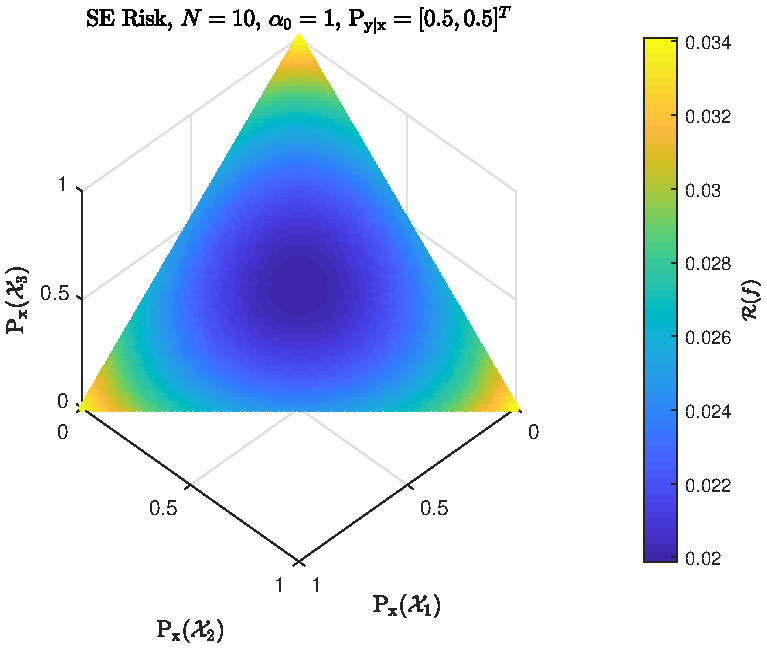
\includegraphics[width=0.7\linewidth]{Risk_SE_Dir_IO_Px_N_10_a0_1.pdf}
\caption{Minimum SE Risk for different PMF's $\Prm(\xrm)$}
\label{fig:Risk_SE_Dir_IO_Px_N_10_a0_1}
\end{figure}

\begin{figure}
\centering
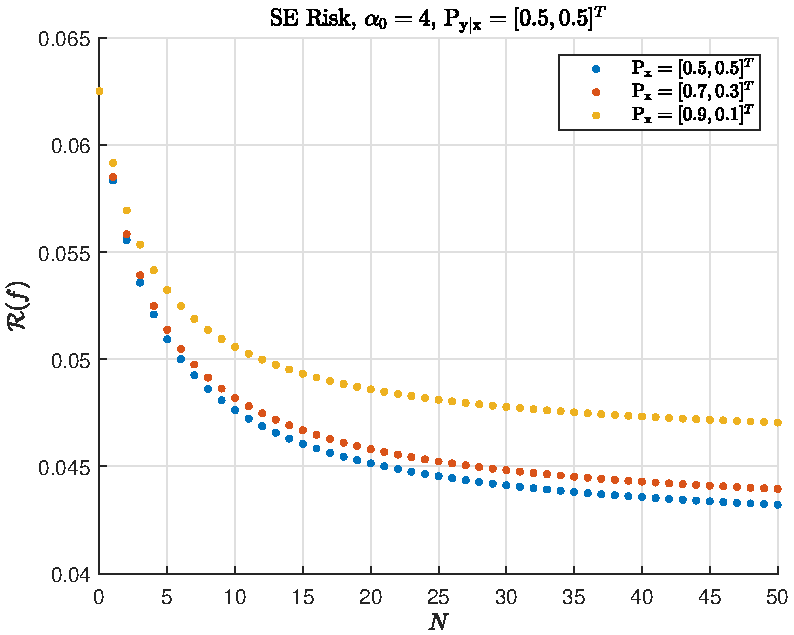
\includegraphics[width=0.7\linewidth]{Risk_SE_Dir_IO_N_leg_Px.pdf}
\caption{Minimum SE Risk for different training set sizes $N$}
\label{fig:Risk_SE_Dir_IO_N_leg_Px}
\end{figure}

\begin{figure}
\centering
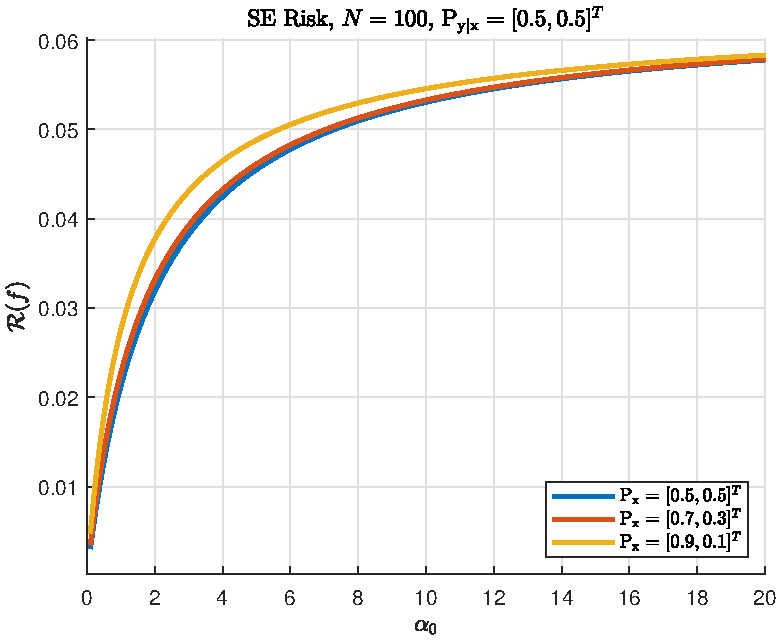
\includegraphics[width=0.7\linewidth]{Risk_SE_Dir_IO_a0_leg_Px.pdf}
\caption{Minimum SE Risk for different prior concentrations $\alpha_0$}
\label{fig:Risk_SE_Dir_IO_a0_leg_Px}
\end{figure}




\subparagraph{Uniform Prior}

The optimal estimator for a uniform prior is
\begin{IEEEeqnarray}{rCl}
f^*(\xrm;\Drm) & = & \left( \frac{|\Ycal|}{N'(\xrm;\Drm) + |\Ycal|} \right) \frac{1}{|\Ycal|} \sum_{y \in \Ycal} y + \left( \frac{N'(\xrm;\Drm)}{N'(\xrm;\Drm) + |\Ycal|} \right) \sum_{y \in \Ycal} y \frac{\bar{N}(y,\xrm;\Drm)}{N'(\xrm;\Drm)} \\
& = & \left( \frac{|\Ycal|}{N'(\xrm;\Drm) + |\Ycal|} \right) \frac{1}{|\Ycal|} \sum_{y \in \Ycal} y + \left( \frac{N'(\xrm;\Drm)}{N'(\xrm;\Drm) + |\Ycal|} \right) \frac{\sum_{n=1}^N \delta\big[ \xrm,\Xrm_n \big] \Yrm_n}{N'(\xrm;\Drm)} \nonumber \;.
\end{IEEEeqnarray}
Now, the model prior contribution to the weighting factors depends on the cardinality $|\Ycal|$ and the prior expectation is simply the average of the elements of $\Ycal$.

For the uniform model prior, the risk reduces to
\begin{IEEEeqnarray}{rCl}
\Rcal^* & = & \frac{1 + \big( N/|\Xcal| + |\Ycal| \big)^{-1}}{1 + |\Ycal|^{-1}} \left[ \left( \frac{1}{|\Ycal|} \sum_{y \in \Ycal} y^2 \right) - \left( \frac{1}{|\Ycal|} \sum_{y \in \Ycal} y \right)^2 \right] \;.
\end{IEEEeqnarray}
Since all possible values of $\xrm$ are equally probable and the conditional probability $\Prm_{\yrm | \xrm}$ is uniform and independent of $\xrm$, the risk simply becomes the variance of the set $\Ycal$ scaled by a factor dependent on $|\Ycal|$ and on $N/|\Xcal|$. Without training data ($N=0$), the scaling is unity; as $N/|\Xcal| \to \infty$, the scaling factor is $\big( 1 + |\Ycal|^{-1} \big)^{-1}$.

To visualize the performance, use the explicit sets $\Ycal$ and $\Xcal$ defined earlier. The conditional variance becomes
\begin{equation}
\Sigma_{\yrm | \xrm} = \frac{|\Ycal|^2 - 1}{12 |\Ycal|^2} = \frac{1 - |\Ycal|^{-2}}{12} 
\end{equation}
and the minimum risk is expressed as
\begin{IEEEeqnarray}{rCl}
\Rcal^* & = & \frac{\big(1 - |\Ycal|^{-1}\big) \Big(1 + \big(N/|\Xcal| + |\Ycal|\big)^{-1} \Big)}{12} \\
& = & \left(\frac{|\Ycal|}{N/|\Xcal| + |\Ycal|}\right) \frac{1 - |\Ycal|^{-2}}{12} + \left(\frac{N/|\Xcal|}{N/|\Xcal| + |\Ycal|}\right) \frac{1 - |\Ycal|^{-1}}{12} \nonumber \;.
\end{IEEEeqnarray}

Interestingly, the minimum squared-error for the uniform prior can be represented as a convex combination of two separate risk values with weighting factors dependent on $|\Ycal|$ and $N/|\Xcal|$. Thus for a uniform prior, the risk depends on the number of elements in $\Ycal$ and the number of training samples ``per element of $\Xcal$''. Note the relationship of these weighting factors to those of the conditional PMF $\Prm_{\yrm | \xrm,\Drm}$, which depend on $\alpha'(\xrm)$ and on $N'(\xrm;\Drm)$. For the uniform prior, $\alpha'(\xrm) = |\Ycal|$ and $\Erm_{\Drm}\big[ N'(\Drm) \big] = N/|\Xcal|$.

The first risk is the conditional variance $\Sigma_{\yrm|\xrm}$ - this is intuitively satisfying as the corresponding weight becomes unity when $N=0$. The second risk is the squared-error with infinite training data. Note that the reduction of the risk between these two extreme cases is modest, and that the attenuating factor increases towards unity for applications with more possible outcomes. Figure \ref{fig:Risk_SE_uniform_N_lim} illustrates the difference between these cases.

\begin{figure}
\centering
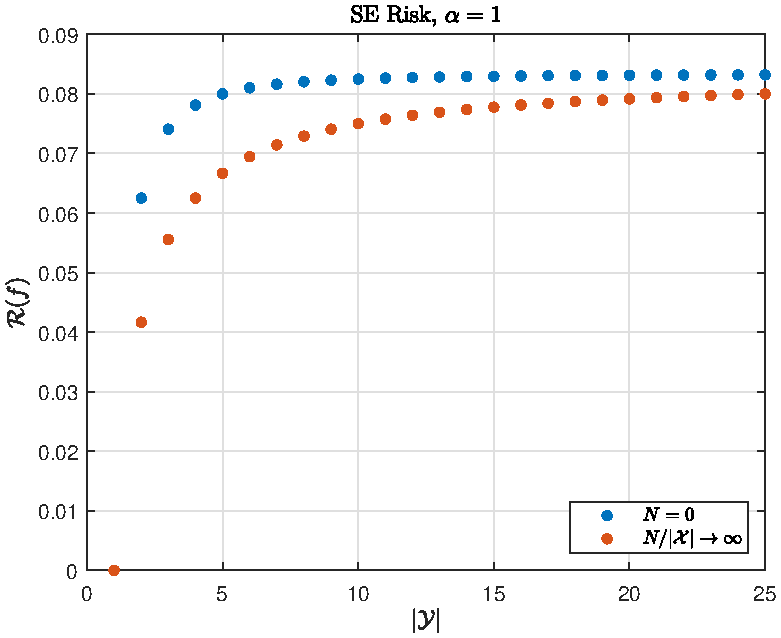
\includegraphics[width=0.7\linewidth]{Risk_SE_uniform_N_lim.pdf}
\caption{Minimum SE Risk, Uniform Prior, zero and infinite training data}
\label{fig:Risk_SE_uniform_N_lim}
\end{figure}





\paragraph{Conditional Squared-Error for a Dirichlet-based Estimator}

Having derived the optimal estimator based on a Dirichlet model prior, it is informative to consider the conditional risk $\Rcal_{\Theta}(f^* ; \uptheta)$ and analyze how different prior parametrizations $\alpha$ influence the squared-error for different models $\theta$. Starting from the conditional squared-error risk \eqref{eq:risk_cond_SE} and substituting the Bayesian estimator \eqref{eq:f_opt_SE}, the formula simplifies to
\begin{IEEEeqnarray}{rCl} \label{eq:risk_cond_SE_dir}
\Rcal_{\Theta}(f^* ; \uptheta) & = & \Rcal_{\Theta}^*(\uptheta) + \Erm_{\xrm,\Drm | \uptheta} \Big[ \big( f^*(\xrm;\Drm) - f_{\Theta}(\xrm;\uptheta) \big)^2 \Big] \\
& = & \Erm_{\xrm | \uptheta} \left[ \Sigma_{\yrm | \xrm,\uptheta} \right] + \Erm_{\xrm,\Drm | \uptheta} \Big[ \big( \mu_{\yrm | \xrm,\Drm} - \mu_{\yrm | \xrm,\uptheta} \big)^2 \Big] \nonumber \;.
\end{IEEEeqnarray}
Defining the excess conditional risk $\Rcal_{\Theta, \mathrm{ex}}(f ; \uptheta) \equiv \Rcal_{\Theta}(f ; \uptheta) - \Rcal_{\Theta}^*(\uptheta)$, the second term above is $\Rcal_{\Theta, \mathrm{ex}}(f^* ; \uptheta) = \Erm_{\xrm,\Drm | \uptheta} \Big[ \big( \mu_{\yrm | \xrm,\Drm} - \mu_{\yrm | \xrm,\uptheta} \big)^2 \Big]$, the average squared bias between the Bayesian predictive mean and the true predictive mean.

Evaluation of the excess risk for an estimator based on the Dirichlet prior will be performed using the sufficient statistic $\nbarrm$ in place of the training set $\Drm$. Using the random process $\Delta(\xrm,\nbarrm,\uptheta) \equiv \Prm_{\yrm | \xrm,\nbarrm} - \Prm_{\yrm | \xrm,\uptheta} \in \Rbb^{\Ycal}$ introduced in \ref{sec:predictive_est}, the term is expressed as
\begin{IEEEeqnarray}{rCl} \label{eq:risk_cond_SE_dir_ex}
\Rcal_{\Theta, \mathrm{ex}}(f^* ; \uptheta) & = & \Erm_{\xrm,\Drm | \uptheta} \Big[ \big( \mu_{\yrm | \xrm,\Drm} - \mu_{\yrm | \xrm,\uptheta} \big)^2 \Big] \\
& = & \sum_{y \in \Ycal} y \sum_{y' \in \Ycal} y' \Erm_{\xrm,\nbarrm | \uptheta} \Big[ \Delta(y;\xrm,\nbarrm,\uptheta) \Delta(y';\xrm,\nbarrm,\uptheta) \Big] \nonumber \\
& = & \sum_{y \in \Ycal} y \sum_{y' \in \Ycal} y' \Erm_{\xrm,\nrm' | \uptheta}\Big[ \mathcal{E}(y,y' ; \xrm,\nrm',\uptheta) \Big] \nonumber \\
& = & \Erm_{\xrm | \uptheta}\left[ \Sigma_{\yrm | \xrm,\uptheta} \Erm_{\nrm'(\xrm) | \uptheta'(\xrm)}\left[ \frac{\nrm'(\xrm)}{\big( \alpha'(\xrm) + \nrm'(\xrm) \big)^2} \right] \right] \nonumber \\
&& \qquad + \Erm_{\xrm | \uptheta}\left[ \left( \mu_{\yrm | \xrm} - \mu_{\yrm | \xrm,\uptheta} \right)^2 \Erm_{\nrm'(\xrm) | \uptheta'(\xrm)}\left[ \left(\frac{\alpha'(\xrm)}{\alpha'(\xrm) + \nrm'(\xrm)}\right)^2 \right] \right] \nonumber \;,
\end{IEEEeqnarray}
where the function $\mathcal{E}$ is defined in \eqref{eq:predictive_del_sq}. 

The excess conditional risk can thus be represented as the conditional expectation (with respect to $\Prm_{\xrm | \uptheta}$) of a sum of two random functions of $\xrm$. The first function measures the additional variance beyond that of the clairvoyant estimator (i.e. the clairvoyant squared-error); like the clairvoyant risk, it depends on $\Sigma_{\yrm | \xrm,\uptheta}$, the conditional variance of the clairvoyant estimate for a given observation of $\xrm$. The second function is dependent on the squared bias between the clairvoyant estimate $\mu_{\yrm | \xrm,\uptheta}$ and the data-independent estimate $\mu_{\yrm | \xrm}$. This term alone is influenced by the data-independent Bayes predictive distribution $\Prm_{\yrm | \xrm} = \alpha(\cdot,\xrm) / \alpha'(\xrm)$.

The two second-order (in terms of $y$) terms are scaled by factors dependent on the prior concentrations $\alpha'(x)$ and on $\uptheta'(x)$ and $N$ via conditional expectations with respect to $\nrm'(x)$. Note that by the aggregation property of multinomial distributions, the random variable $\nrm'(x) | \uptheta'(x) \sim \Bi \big(N,\uptheta'(x)\big)$. Closed-forms have not been found for the function expectations of binomial random variables above.


It is informative to consider the trends in the conditional squared-error risk \eqref{eq:risk_cond_SE_dir_ex} for different volumes of training data $N$ and for different selections of $\alpha$. First consider how the excess risk changes with the training volume $N$. For $N=0$, it is evident that the excess risk is $\Rcal_{\Theta, \mathrm{ex}}(f^* ; \uptheta) \to \Erm_{\xrm | \uptheta}\left[ \left( \mu_{\yrm | \xrm} - \mu_{\yrm | \xrm,\uptheta} \right)^2 \right]$,  the expected squared bias between the clairvoyant and data-independent estimators. As $N$ tends to infinity, the binomial distribution controlling the scaling factors  concentrates at $\nrm'(x) \approx N \theta'(x)$; as such, the two expectations of interest tend to zero and thus $\Rcal_{\Theta, \mathrm{ex}}(f^* ; \uptheta) \to 0$. This desirable property of the estimator is a consequence of the full support of the Dirichlet prior, ensuring that the model posterior concentrates at the empirical PMF.

Another interesting point regarding the depedency of the excess conditional risk on $N$ is that, depending on the learner parameterization, there may be a local maximum. Consider the trivial case of $|\Xcal| = 1$ - treating $N$ as a real number, there would be a maximum at 
\begin{equation}
N \equiv \alpha'(x) \left( 1 - 2 \alpha'(x) \frac{\left( \mu_{\yrm | \xrm} - \mu_{\yrm | \xrm,\uptheta} \right)^2}{\Sigma_{\yrm | \xrm,\uptheta}} \right) \;.
\end{equation}
Note that as the squared-difference between the prior mean and true mean increases, the maximizing value decreases (even below zero). Thus, the worse the prior estimate, the more likely the excess squared-error will decrease monotonically with $N$. Conversely, if the prior estimate is accurate, a local maximum may occur and additional training data may (temporarily) compromize the estimator performance. Also consider the effect of prior concentration; informative priors with sufficiently high $\alpha'(x)$ will not have the local maxima.

The excess risk at this potentially non-integral value would be 
\begin{equation}
\Rcal_{\Theta, \mathrm{ex}}(f^* ; \uptheta) \to \Erm_{\xrm | \uptheta}\left[ \frac{\frac{1}{\alpha'(\xrm)} - \frac{\left( \mu_{\yrm | \xrm} - \mu_{\yrm | \xrm,\uptheta} \right)^2}{\Sigma_{\yrm | \xrm,\uptheta}}}{4\left( 1 - \frac{\left( \mu_{\yrm | \xrm} - \mu_{\yrm | \xrm,\uptheta} \right)^2}{\Sigma_{\yrm | \xrm,\uptheta}} \right)} \Sigma_{\yrm | \xrm,\uptheta} \right] \;.
\end{equation}

Figures \ref{fig:Risk_cond_SE_Dir_N_leg_a0_unbiased} and \ref{fig:Risk_cond_SE_Dir_N_leg_a0_biased} exemplify the excess conditional squared-error as a function of $N$ for estimators based on Dirichlet priors of varying concentration $\alpha'(x)$. The former shows local maxima for an unbiased estimator; note that higher concentration results in superior performance. The latter uses biased estimators and as such, learners based on low concentration achieve lower risk.
\begin{figure}
\centering
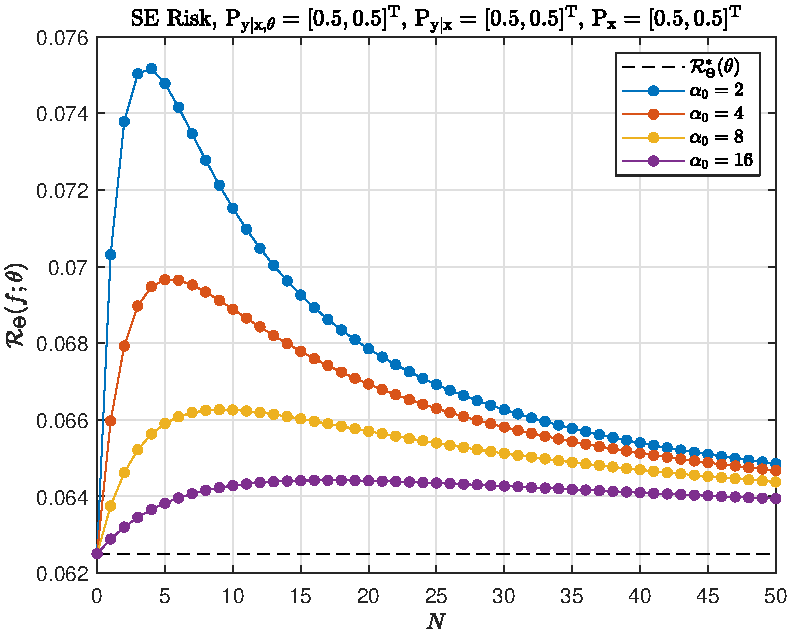
\includegraphics[width=0.7\linewidth]{Risk_cond_SE_Dir_N_leg_a0_unbiased.pdf}
\caption{Conditional SE Risk versus $N$, unbiased Dirichlet estimators of varying concentration}
\label{fig:Risk_cond_SE_Dir_N_leg_a0_unbiased}
\end{figure}
\begin{figure}
\centering
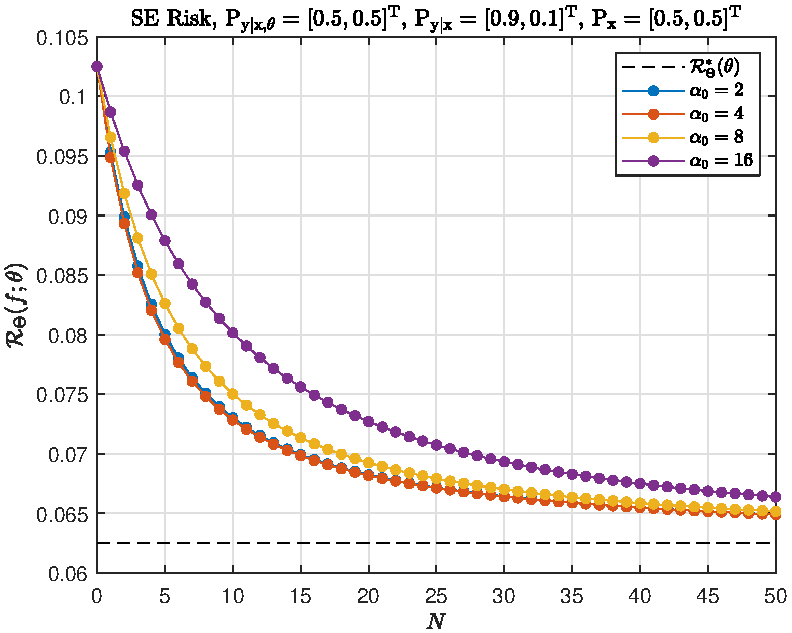
\includegraphics[width=0.7\linewidth]{Risk_cond_SE_Dir_N_leg_a0_biased.pdf}
\caption{Conditional SE Risk versus $N$, biased Dirichlet estimators of varying concentration}
\label{fig:Risk_cond_SE_Dir_N_leg_a0_biased}
\end{figure}







Next consider the effects of the Dirichlet prior parameters. The analysis will interpret the Dirichlet parameters as the conditional prior distributions $\alpha(\cdot,x)/\alpha'(x)$ and their concentrations $\alpha'(x)$. 

First consider the conditional prior PMF's $\alpha(\cdot,x) / \alpha'(x)$; as shown, they manifest themselves in the risk through the squared estimator bias. It is clear that regardless of how the values $\alpha'(x)$ are chosen, the best selections for these conditional priors must have first moments matching those of the corresponding clarivoyant predictive distrbutions $\Prm_{\yrm | \xrm,\uptheta}$ for each $x \in \Xcal$. Such estimators are unbiased; as a result, the excess conditional risk is thus equivalent to the first term in \eqref{eq:risk_cond_SE_dir_ex}, measuring additional variance due to model uncertainty.



The other user-selected Dirichlet parameters $\alpha'(x)$ are the concentration parameters for the corresponding conditional distributions; they control important bias/variance trade-offs via the two scaling factors in \eqref{eq:risk_cond_SE_dir_ex}. First, consider the asymptotic trends.

Consider how the excess risk tends as the priors become maximally concentrated. As the parameters $\alpha'(x) \to \infty$, the excess risk tends to $\Rcal_{\Theta, \mathrm{ex}}(f^* ; \uptheta) \to \Erm_{\xrm | \uptheta}\left[ \left( \mu_{\yrm | \xrm} - \mu_{\yrm | \xrm,\uptheta} \right)^2 \right]$, the expected conditional squared-error between the means of the Bayesian predicitve PMF and the clairvoyant predictive PMF. This is intuitive given that the estimator tends toward a data-independent solution; analagous to the discussion in Section \ref{sec:predictive_est}, the estimator may be biased, but will have no variance due to the training data statistics.

Conversely, if concentrations $\alpha'(x) \to 0$ are chosen, the Bayesian estimate tends to the empirical mean, independent of $\alpha(\cdot,\xrm) / \alpha'(\xrm)$, and the excess risk tends to
\begin{IEEEeqnarray}{rCl}
\Rcal_{\Theta, \mathrm{ex}}(f^* ; \uptheta) & \to & \Erm_{\xrm | \uptheta}\left[ \Sigma_{\yrm | \xrm,\uptheta} \sum_{n=1}^N \binom{N}{n} \uptheta'(\xrm)^n \big( 1 - \uptheta'(\xrm) \big)^{N-n} \frac{1}{n} \right] \nonumber \\
&& \qquad + \Erm_{\xrm | \uptheta}\left[ \big( 1 - \uptheta'(\xrm) \big)^N \left( \mu_{\yrm | \xrm} - \mu_{\yrm | \xrm,\uptheta} \right)^2 \right] \nonumber \;.
\end{IEEEeqnarray}
Note that the first term's scaling factor is proportionate to the first inverse moment of a positive binomial random variable \cite{stephan}. The second term's scaling factor tends to $\Prm_{\nrm'(\xrm) | \uptheta'(\xrm)}\big( 0 | \theta'(x) \big)$, the probability that no training samples are observed matching the value $\xrm$. As $N$ increases, this term tends to zero, the risk due to the prior estimate bias decreases, and the excess risk becomes a function of $\uptheta$ only.



Of further interest are the values $\alpha'(x)$ that minimize the excesss squared-error for a given prior conditional distribution $\alpha(\cdot,x) / \alpha'(x)$. With the asymptotic values of the excess risk known, all that remains is to determine any local minima. Since the excess risk is a sum of $|\Xcal|$ terms of identical form, each dependent on their own concentration $\alpha'(x)$, only one component needs to be minimized. 

Calculating the first derivative with respect to $\alpha'(x)$, it can be shown that for $N > 0$ and $\theta'(x) > 0$, only one stationary point exists, at 
\begin{equation} \label{eq:alpha_x_min_Rex}
\alpha'(x) \equiv \frac{\Sigma_{\yrm | \xrm,\uptheta}}{\left( \mu_{\yrm | \xrm} - \mu_{\yrm | \xrm,\uptheta} \right)^2} \;.
\end{equation}
Calculation of the second derivative confirms that this value is a local minimum. Furthermore, the excess risk evaluated at these values is 
\begin{equation}
\Rcal_{\Theta, \mathrm{ex}}(f^* ; \uptheta) = \Erm_{\xrm | \uptheta}\left[ \Erm_{\nrm'(\xrm) | \uptheta'(\xrm)}\left[ \frac{1}{\nrm'(\xrm)\Sigma_{\yrm | \xrm,\uptheta}^{-1} + \left( \mu_{\yrm | \xrm} - \mu_{\yrm | \xrm,\uptheta} \right)^{-2}} \right] \right] \;,
\end{equation}
which can be easily shown to be less than both the asymptotic values for $\alpha'(x) \to 0$ and $\alpha'(x) \to \infty$. Thus the concentation values \eqref{eq:alpha_x_min_Rex} provide the minimum excess risk for the given prior conditional distributions.

Note that the minimizing concentration values $\alpha'(x)$ are inversely proportional to the squared-bias of the prior conditional mean. This is sensible; the better the match between the true and prior predictive distributions, the more confidence should be expressed. Also, low concentrations are preferable when the model has low conditional variance; these models can be quickly identified with learners prioritizing the emprical PMF estimate over the prior estimate. Additionally, note that these values $\alpha'(x)$ do not depend on the training volume $N$.




Figures \ref{fig:Risk_cond_SE_Dir_a0_leg_N_unbiased} and \ref{fig:Risk_cond_SE_Dir_a0_leg_N_biased} show how the excess conditional squared-error trends as a function of the Dirichlet learner concentration. Note that the latter is based on a biased prior estimate and thus the optimal Dirichlet concentration value is lower.
\begin{figure}
\centering
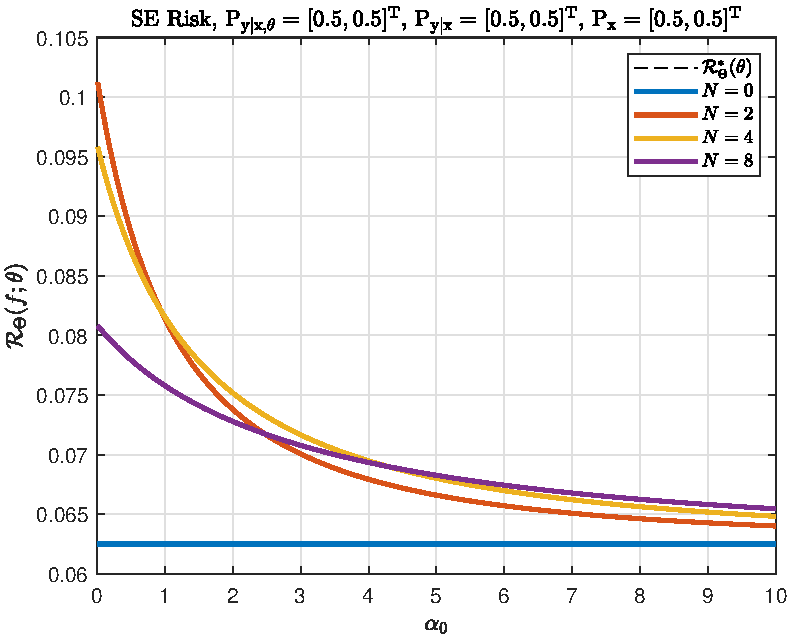
\includegraphics[width=0.7\linewidth]{Risk_cond_SE_Dir_a0_leg_N_unbiased.pdf}
\caption{Conditional SE Risk versus $\alpha'(x)$, unbiased Dirichlet estimator using varying training set volumes}
\label{fig:Risk_cond_SE_Dir_a0_leg_N_unbiased}
\end{figure}
\begin{figure}
\centering
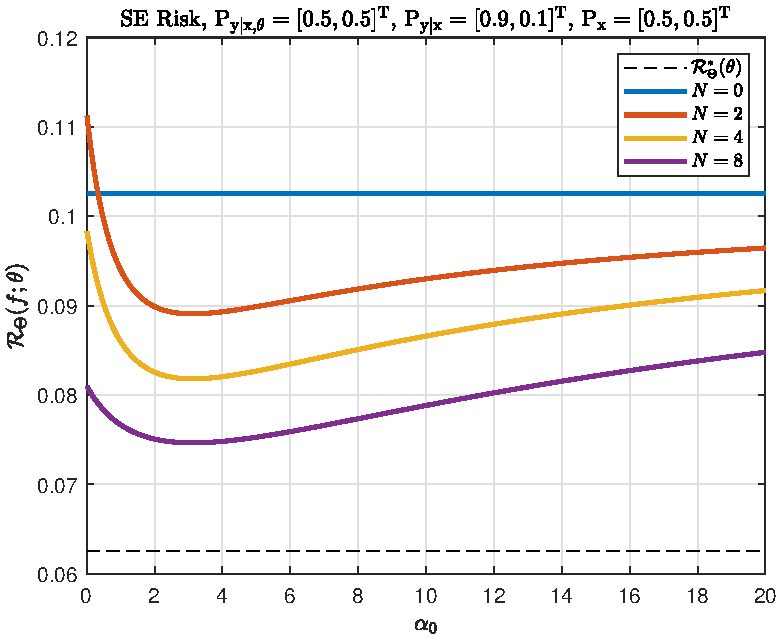
\includegraphics[width=0.7\linewidth]{Risk_cond_SE_Dir_a0_leg_N_biased.pdf}
\caption{Conditional SE Risk versus $\alpha'(x)$, biased Dirichlet estimator using varying training set volumes}
\label{fig:Risk_cond_SE_Dir_a0_leg_N_biased}
\end{figure}











\subsubsection{Classification: the 0-1 Loss}

This section derives 0-1 loss classifiers based on the Dirichlet prior distribution and assesses their performance.

\paragraph{Bayesian Classification}

To determine the optimal learning function, the 0-1 loss from Equation \eqref{eq:loss_01} is substituted into Equation \eqref{eq:E_y|xD L} and Equation \eqref{eq:f_opt_xD} to find
\begin{IEEEeqnarray}{rCl} \label{eq:f_opt_01_dir}
f^*(\xrm;\Drm) & = & \argmax_{y \in \Ycal} \Prm_{\yrm | \xrm,\Drm}(y | \xrm,\Drm) \\
& = & \argmax_{y \in \Ycal} \frac{\alpha(y,\xrm) + \bar{N}(y,\xrm;\Drm)}{\alpha'(\xrm) + N'(\xrm;\Drm)} \nonumber \\
& = & \argmax_{y \in \Ycal} \left( \alpha(y,\xrm) + \bar{N}(y,\xrm;\Drm) \right) \nonumber \;.
\end{IEEEeqnarray}
Using the Dirichlet prior, different classes are ``scored'' by counting the number of training samples with a value of $\Xrm_n$ matching that of $\xrm$ and combining with the prior parameters $\alpha(\cdot,\xrm)$.  

Evaluating the minimum risk \eqref{eq:risk_min_01} using the distributions derived from the Dirichlet prior, the Bayes minimum probability of error is 
\begin{IEEEeqnarray}{rCl}
\Rcal^* & = & 1 - \Erm_{\xrm,\Drm} \left[ \max_{y \in \Ycal} \Prm_{\yrm | \xrm,\Drm}(y | \xrm,\Drm) \right] \\
& = & 1 - \Erm_{\xrm,\nbarrm} \left[ \frac{ \max_{y \in \Ycal} \big( \alpha(y,x) + \bar{\nrm}(y,x) \big)}{\alpha'(x) + \nrm'(x)} \right] \nonumber \\
& = & 1 - \sum_{x \in \Xcal} \frac{\Erm_{\nbarrm} \Big[ \max_{y \in \Ycal} \big( \alpha(y,x) + \bar{\nrm}(y,x) \big) \Big]}{\alpha_0 + N} \nonumber \;.
\end{IEEEeqnarray}

Figures \ref{fig:Risk_01_Dir_N_leg_a0} and \ref{fig:Risk_01_Dir_a0_leg_N} plot the minimum Bayes probability of error against training data volume $N$ and prior concentration $\alpha_0$, respectively. Note that for $N = 0$, the Bayes risk is $\Rcal^* = 1 - \sum_{x \in \Xcal} \frac{\max_{y \in \Ycal} \alpha(y,x)}{\alpha_0}$. Additionally, consider the risk for maximal/minimal values of the Dirichlet concentration. For $\alpha_0 \to 0$ (and $N > 1$), the risk is $\Rcal^* = 0$; conversely, for $\alpha_0 \to \infty$, the risk tends to $\Rcal^* \to 1 - \sum_{x \in \Xcal} \frac{\max_{y \in \Ycal} \alpha(y,x)}{\alpha_0}$. These trends can be visualized in Figures \ref{fig:Risk_01_Dir_Pyx__a0_high} and \ref{fig:Risk_01_Dir_Pyx__a0_low}.
%
\begin{figure}
\centering
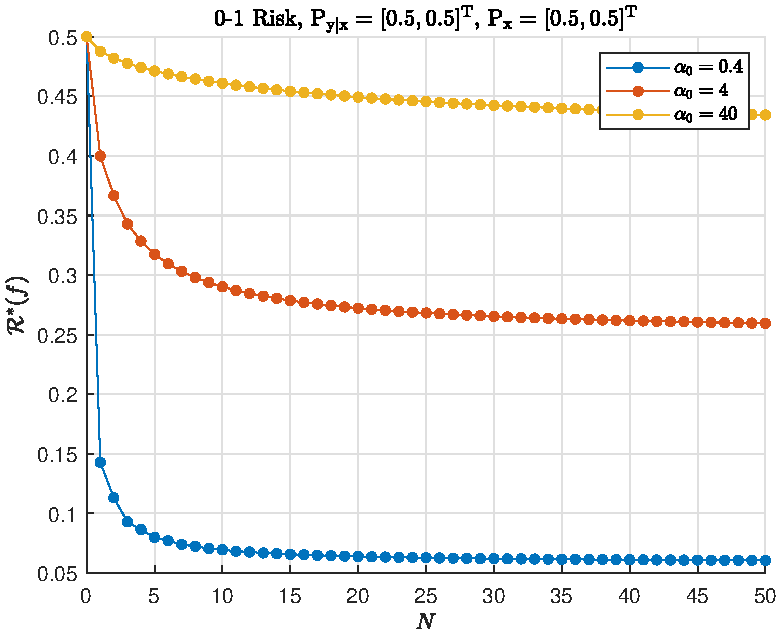
\includegraphics[width=0.7\linewidth]{Risk_01_Dir_N_leg_a0.pdf}
\caption{Minimum 0-1 Risk for different training data volumes $N$}
\label{fig:Risk_01_Dir_N_leg_a0}
\end{figure}
%
\begin{figure}
\centering
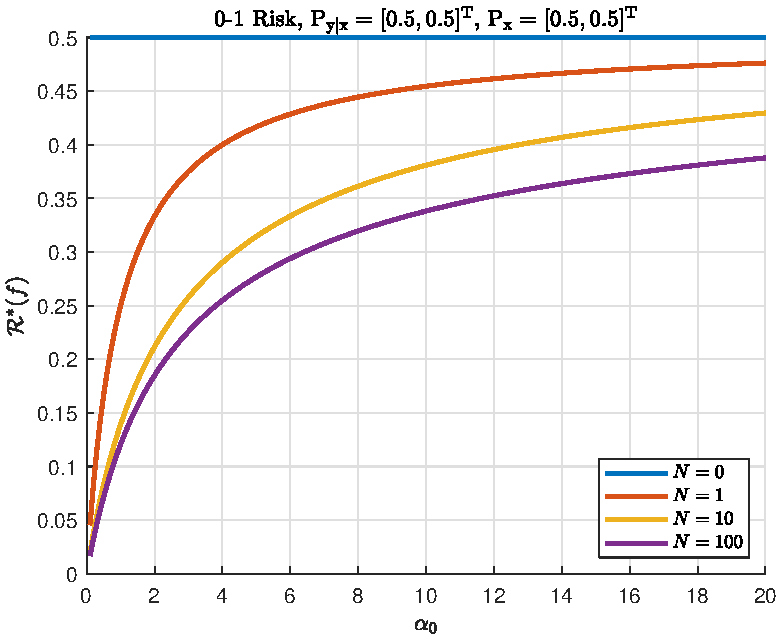
\includegraphics[width=0.7\linewidth]{Risk_01_Dir_a0_leg_N.pdf}
\caption{Minimum 0-1 Risk for different prior concentrations $\alpha_0$}
\label{fig:Risk_01_Dir_a0_leg_N}
\end{figure}
%
\begin{figure}
\centering
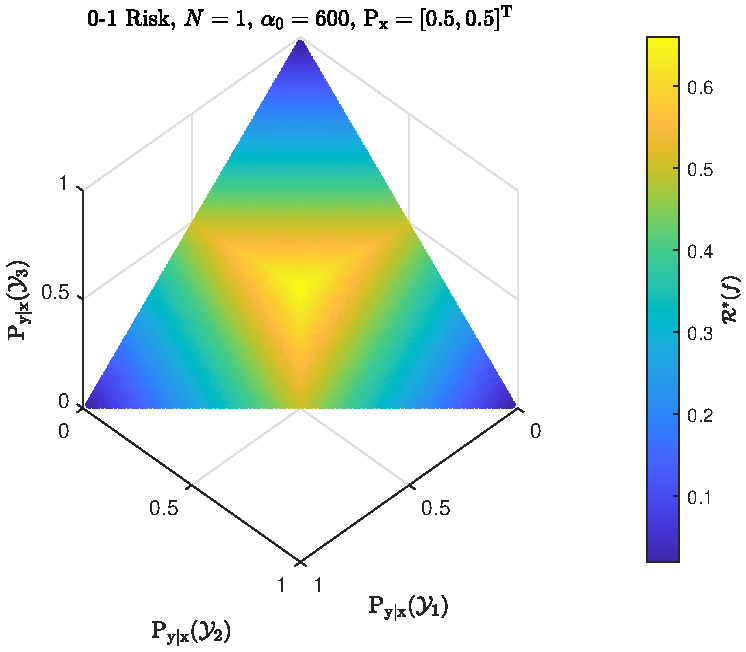
\includegraphics[width=0.7\linewidth]{Risk_01_Dir_Pyx__a0_high.pdf}
\caption{Minimum 0-1 Risk for different prior means $\Prm_{\yrm | \xrm}$}
\label{fig:Risk_01_Dir_Pyx__a0_high}
\end{figure}
%
\begin{figure}
\centering
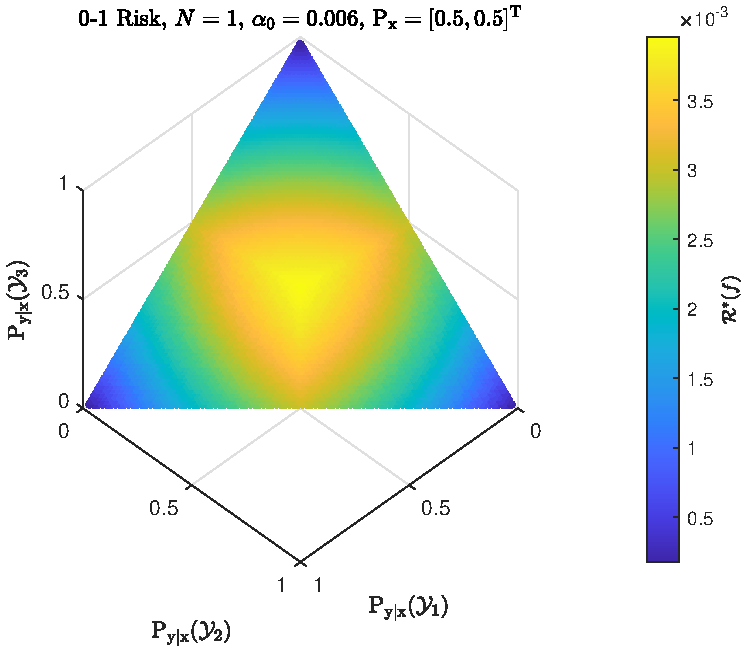
\includegraphics[width=0.7\linewidth]{Risk_01_Dir_Pyx__a0_low.pdf}
\caption{Minimum 0-1 Risk for different prior means $\Prm_{\yrm | \xrm}$}
\label{fig:Risk_01_Dir_Pyx__a0_low}
\end{figure}








\subparagraph{Uniform Prior}

When the uniform prior is used, the Bayes classifier simplifies to 
\begin{IEEEeqnarray}{rCl}
f^*(\xrm;\Drm) & = & \argmax_{y \in \Ycal} \bar{N}(y,\xrm;\Drm) \;,
\end{IEEEeqnarray}
a conditional majority decision which chooses the class from $\Ycal$ most often represented among training set samples $\Drm$ with a matching input value $\xrm$. This is intuitive, as the model PDF parameter $\alpha$ imparts no confidence as to which classes may be most likely.


Using the uniform prior, the minimum Bayes 0-1 risk is 
\begin{IEEEeqnarray}{rCl}
\Rcal^* & = & 1 - \Erm_{\xrm,\Drm} \left[ \max_{y \in \Ycal} \Prm_{\yrm | \xrm,\Drm}(y | \xrm,\Drm) \right] \\
& = & 1 - \frac{1 + |\Xcal|^{-1} \sum_{x \in \Xcal} \Erm_{\nbarrm} \big[ \max_{y \in \Ycal} \bar{\nrm}(y,x) \big]}{|\Ycal| + N/|\Xcal|} \nonumber \;.
\end{IEEEeqnarray}
The expectation operates on the maximum value from a subset of a uniform Dirichlet-Multinomial random process. Via the Dirichlet-Multinomial aggregation property \cite{johnson}, a consequence of the the uniform PMF $\Prm_{\nbarrm}$ is that the individual segments $\nbarrm(\cdot,x)$ are identically distributed; thus, the expectation will be same for every value $x$.

To evaluate this expectation, new random variables $\nbarrm_{\max}(x) \equiv \max_{y \in \Ycal} \nbarrm(y,x)$ are introduced and characterized by their identical PMF. To this end, the probability of the event $\Prm\big( \nbarrm_{\max}(x) \geq n \big) = \Prm\big( \cup_{y \in \Ycal} \{ \nbarrm(y,x) \geq n \} \big)$ will be determined. As the distribution of $\nbarrm$ is uniform, the event probability is proportionate to the cardinality of the set $\cup_{y \in \Ycal} \{ \bar{n}: \bar{n}(y,x) \geq n \}$. Using the inclusion-exclusion principle \cite{brualdi}, the cardinality is represented as
\begin{IEEEeqnarray}{L}
\big| \cup_{y \in \Ycal} \{ \bar{n} : \bar{n}(y,x) \geq n \} \big| \\
\quad = \begin{cases} \binom{N+|\Ycal||\Xcal|-1}{|\Ycal||\Xcal|-1} & \mathrm{if} \ n < 0, \\ \sum_{m=1}^{|\Ycal|} \binom{|\Ycal|}{m} (-1)^{m-1} \binom{N-mn+|\Ycal||\Xcal|-1}{|\Ycal||\Xcal|-1} H\Big( \big\lfloor\frac{N}{m}\big\rfloor - n \Big) & \mathrm{if} \ 0 \leq n \leq N, \\ 0 & \mathrm{if} \ n > N, \end{cases} \nonumber
\end{IEEEeqnarray}
where $H: \Zbb \mapsto \{0,1\}$ is the discrete Heaviside step function. For $n < 0$, the cardinality is equivalent to $|\bar{\Ncal}|$. 

For $0 \leq n < N$, the cardinality is an alternating binomial summation where the $m^\mathrm{th}$ term accounts for the different intersections of $m$ of the $|\Ycal|$ individual sets $\{ \bar{n} : \bar{n}(y,x) \geq n \}$. Observe that the cardinality of the intersections is only dependent on the number of contributing sets $m$ and not on which sets intersect. Furthermore, note the dependency of the intersection cardinalities on the argument $n$. The step function contributes such that if $n > \big\lfloor\frac{N}{m}\big\rfloor$, only up to $m-1$ individual sets will intersect. The binomial coefficient $\Mcal\big( \{N-mn,|\Ycal||\Xcal|-1\} \big)$ provides the intersection cardinality for a given $m$; note the similarity to the cardinality $|\bar{\Ncal}|$ - the only difference is the number of points characterizing the $|\Ycal||\Xcal|-1$ dimensional region.

The probability of interest can thus be expressed as
\begin{IEEEeqnarray}{L}
\Prm\big( \nbarrm_{\max}(x) \geq n \big) = \binom{N+|\Ycal||\Xcal|-1}{|\Ycal||\Xcal|-1}^{-1} \big| \cup_{y \in \Ycal} \{ \bar{n} : \bar{n}(y,x) \geq n \} \big| \\
\quad = \begin{cases} 1 & \mathrm{if} \ n < 0, \\ \sum_{m=1}^{|\Ycal|} \binom{|\Ycal|}{m} (-1)^{m-1} \prod_{l=1}^{|\Ycal||\Xcal|-1} \Big( 1-\frac{mn}{N+l} \Big) H\Big( \big\lfloor\frac{N}{m}\big\rfloor - n \Big) & \mathrm{if} \ 0 \leq n \leq N, \\ 0 & \mathrm{if} \ n > N. \end{cases} \nonumber
\end{IEEEeqnarray}


As the PMF of $\nbarrm_{\max}(x)$ has support on $n \in [0,\ldots,N]$, the expectation over $\nbarrm$ is evaluated as
\begin{IEEEeqnarray}{rCl}
\Erm_{\nbarrm}\big[ \nbarrm_{\max}(x) \big] & = & \sum_{n=0}^N n \Big( \Prm\big( \nbarrm_{\max}(x) \geq n \big) - \Prm\big( \nbarrm_{\max}(x) \geq n+1 \big) \Big) \\
& = & -1 + \sum_{n=0}^N \Prm\big( \nbarrm_{\max}(x) \geq n \big) \nonumber \\
& = & -1 + \sum_{m=1}^{|\Ycal|} \binom{|\Ycal|}{m} (-1)^{m-1} \sum_{n=0}^{\big\lfloor\frac{N}{m}\big\rfloor} \prod_{l=1}^{|\Ycal||\Xcal|-1} \Big( 1-\frac{mn}{N+l} \Big) \nonumber 
\end{IEEEeqnarray}
and the minimum 0-1 risk is
\begin{IEEEeqnarray}{rCl}
\Rcal^* & = & 1 - \frac{\sum_{m=1}^{|\Ycal|} \binom{|\Ycal|}{m} (-1)^{m-1} \sum_{n=0}^{\big\lfloor\frac{N}{m}\big\rfloor} \prod_{l=1}^{|\Ycal||\Xcal|-1} \Big( 1-\frac{mn}{N+l} \Big)}{|\Ycal| + N/|\Xcal|} \; .
\end{IEEEeqnarray}




It is informative to express the risk for minimal and maximal volumes of training data. Using the binomial summation identity 
\begin{equation}
\sum_{m=0}^M \binom{M}{m} (-1)^m g(m) = 0 \; ,
\end{equation}
where $g$ is a polynomial function of degree less than $M$ \cite{graham}, it can be shown that for $N = 0$, the minimum risk is $\Rcal^*  = 1 - |\Ycal|^{-1}$. This is sensible, as the classes are equiprobable with $\Prm_{\yrm} = |\Ycal|^{-1}$.


To find the risk for $N \to \infty$, note that
\begin{IEEEeqnarray}{L}
\lim_{N \to \infty} \big( |\Ycal| + N/|\Xcal| \big)^{-1} \sum_{n=0}^{\big\lfloor\frac{N}{m}\big\rfloor} \prod_{l=1}^{|\Ycal||\Xcal|-1} \Big( 1-\frac{mn}{N+l} \Big) \\
\qquad = \lim_{N/m \to \infty} \frac{|\Xcal|}{m} \sum_{n=0}^{\big\lfloor\frac{N}{m}\big\rfloor} \left( 1 - \frac{mn}{N} \right)^{|\Ycal||\Xcal|-1} \frac{m}{N} \nonumber \\
\qquad = \frac{|\Xcal|}{m} \int_0^1 (1-t)^{|\Ycal||\Xcal|-1} \mathrm{d} t \nonumber \\
\qquad = \frac{1}{m|\Ycal|} \nonumber \;.
\end{IEEEeqnarray}
The irreducible 0-1 risk for the uniform prior tends toward
\begin{IEEEeqnarray}{rCl}
\Rcal^* & \to & 1 - |\Ycal|^{-1} \sum_{m=1}^{|\Ycal|} \binom{|\Ycal|}{m} (-1)^{m-1} m^{-1} \\
& = & 1 - |\Ycal|^{-1} \sum_{m=1}^{|\Ycal|} m^{-1} \nonumber \;,
\end{IEEEeqnarray}
providing a lower bound for the achievable 0-1 Bayes risk. The above formulation has made use of the alternating summation identity from \cite{roman} to display the risk with a form including the $|\Ycal|^\mathrm{th}$ harmonic number $H_{|\Ycal|} \equiv \sum_{m=1}^{|\Ycal|} m^{-1}$. Observe that the irreducible risk does not depend on the cardinality $|\Xcal|$.



Figure \ref{fig:Risk_01_uni_N_leg_My} demonstrates how the minimum 0-1 risk decreases with training volume $N$; observe that the risk is more severe for sequences corresponding to higher $|\Ycal|$. It is sensible that the probability of error should increase when more classes have to be considered. Figure \ref{fig:Risk_01_uni_N_leg_Mx} illustrates the minimum risk with multiple sequences for different cardinalities $|\Xcal|$. Note that risk increases with $|\Xcal|$. Considering $\Erm_{\Drm}\big[N'(\Drm)\big] = \mu_{\nrm'} = N/|\Xcal|$, this should be intuitive - each conditional empirical distribution $\bar{N}(\cdot,x;D) / N'(x;D)$ is forced to approximate $\tilde{\uptheta}(x)$ with less data.

\begin{figure}
\centering
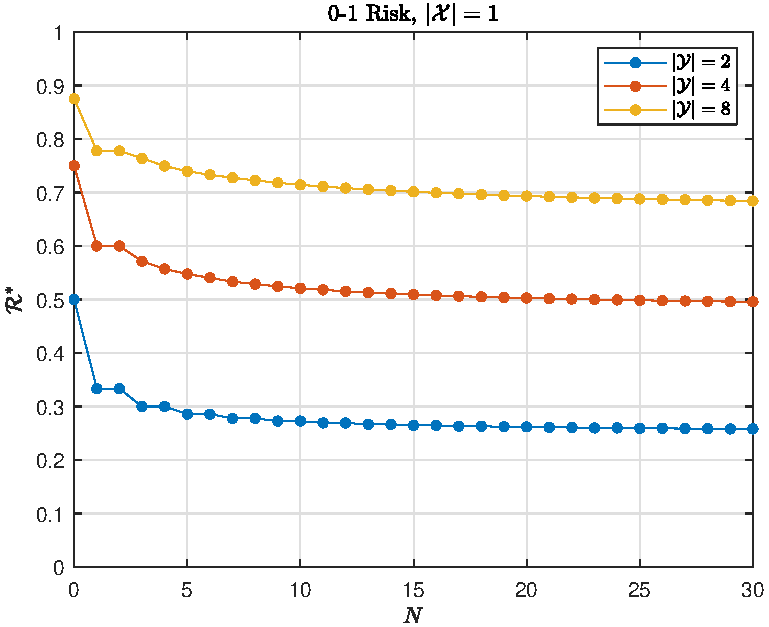
\includegraphics[width=0.7\linewidth]{Risk_01_uni_N_leg_My.pdf}
\caption{Minimum 0-1 Risk vs training set volume $N$}
\label{fig:Risk_01_uni_N_leg_My}
\end{figure}

\begin{figure}
\centering
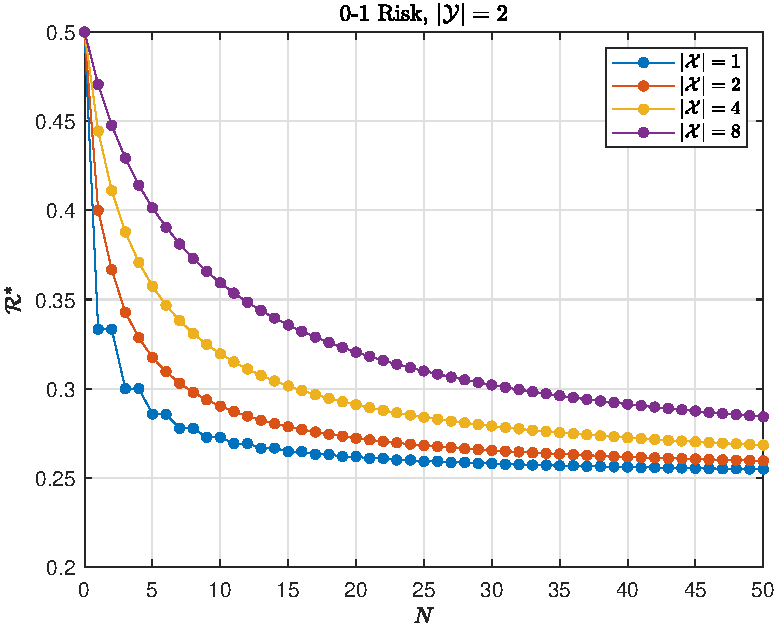
\includegraphics[width=0.7\linewidth]{Risk_01_uni_N_leg_Mx.pdf}
\caption{Minimum 0-1 Risk vs training set volume $N$}
\label{fig:Risk_01_uni_N_leg_Mx}
\end{figure}

Further insight into how $|\Xcal|$ affects the risk can be acquired by plotting the risk as a function of $N/|\Xcal|$. In Figure \ref{fig:Risk_01_uni_N-Mx}, it is shown that the optimal risk can be approximated by a function dependent only on $N/|\Xcal|$; of the series plotted, only the series for $|\Xcal| = 1$ shows notable non-negligible from the others.

\begin{figure}
\centering
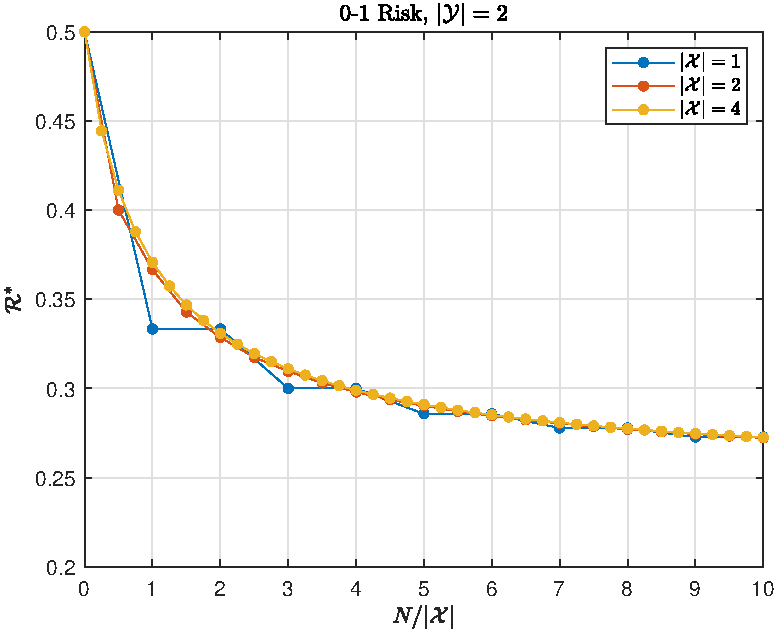
\includegraphics[width=0.7\linewidth]{Risk_01_uni_N-Mx.pdf}
\caption{Minimum 0-1 Risk vs $N/|\Xcal|$}
\label{fig:Risk_01_uni_N-Mx}
\end{figure}


It is also informative to graph the $N=0$ and $N \to \infty$ minimum risk as a function of $|\Ycal|$; both formulas are independent of $|\Xcal|$. Figure \ref{fig:Risk_01_uni_N_bounds} displays these bounds; note the margin in the probability of error between the optimal $N=0$ and $N \to \infty$ classifiers. For $|\Ycal| = 2$ binary classification, both sequences are at their minimum and infinite training data provides a reduction in expected probability of error from 0.5 to 0.25. As $|\Ycal|$ increases, the classification risk for both the $N=0$ and $N \to \infty$ cases tend to unity and the error reduction for $N \to \infty$ decreases. 





\begin{figure}
\centering
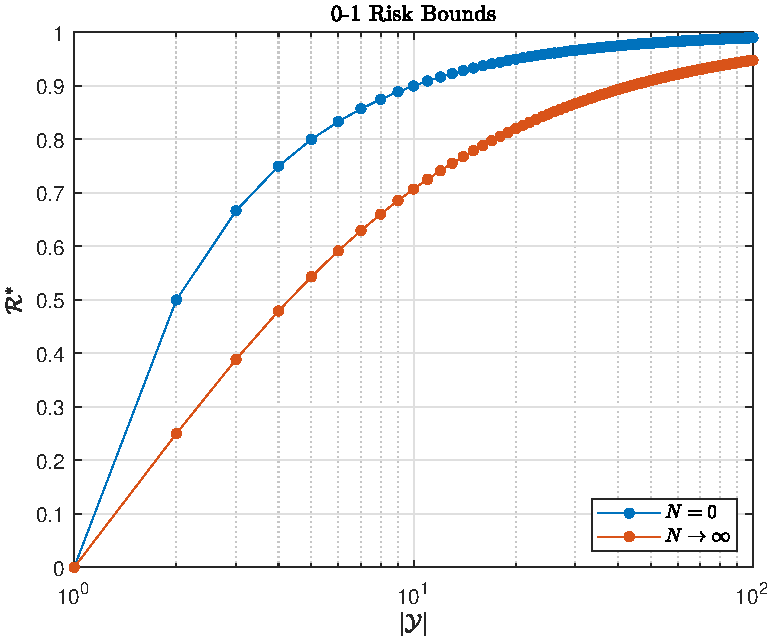
\includegraphics[width=0.7\linewidth]{Risk_01_uni_N_bounds.pdf}
\caption{Minimum 0-1 Risk vs $|\Ycal|$}
\label{fig:Risk_01_uni_N_bounds}
\end{figure}






\paragraph{Conditional Probability of Error for a Dirichlet-based Classifier}


Substituting the optimal Dirichlet-based classifier into the formula for the conditional probability of error \ref{eq:risk_cond_01}, the risk is
\begin{IEEEeqnarray}{rCl}
\Rcal_{\Theta}(f ; \uptheta) & = & 1 - \sum_{x \in \Xcal} \uptheta'(x) \Erm_{\nbarrm | \uptheta} \bigg[ \tilde{\uptheta}\Big( \max_{y \in \Ycal} \big( \nbarrm(y,x) + \alpha(y,x) \big) ;x \Big) \bigg] \;.
\end{IEEEeqnarray}
Figures \ref{fig:Risk_cond_01_Dir_N_leg_a0__subj_good} and \ref{fig:Risk_cond_01_Dir_N_leg_a0__subj_bad} show how the conditional risk trends for classifiers based on well-matched and poorly-matched informative Dirichlet priors, respectively. Note that the well-matched prior does better with higher prior concentrations $\alpha_0$; this is reflective of the fact that the maximizing arguments $y \in \Ycal$ of both the true model $\tilde{\theta}(x)$ and the prior mean $\alpha(\cdot,x) / \alpha'(x)$ are the same.
\begin{figure}
\centering
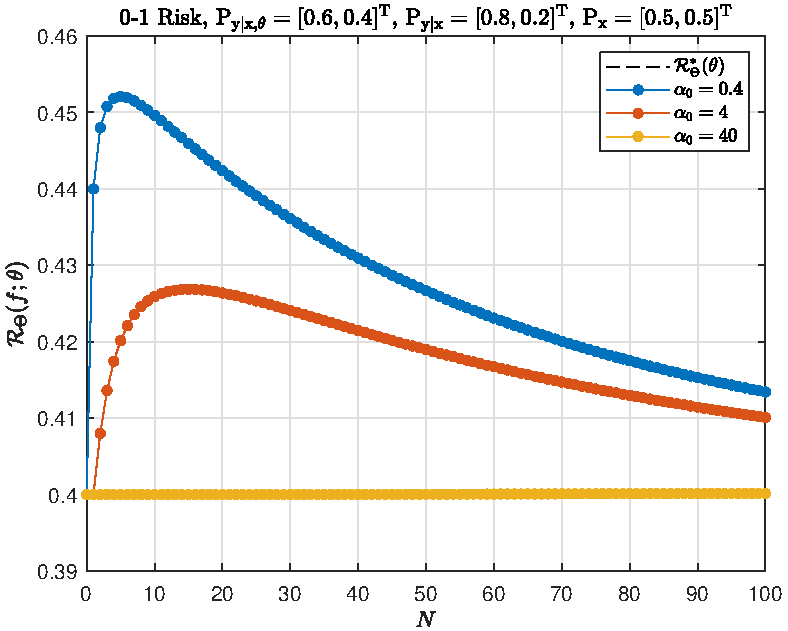
\includegraphics[width=0.7\linewidth]{Risk_cond_01_Dir_N_leg_a0__subj_good.pdf}
\caption{Excess conditional probability of error, well-matched informative Dirichlet-based classifier}
\label{fig:Risk_cond_01_Dir_N_leg_a0__subj_good}
\end{figure}
%
\begin{figure}
\centering
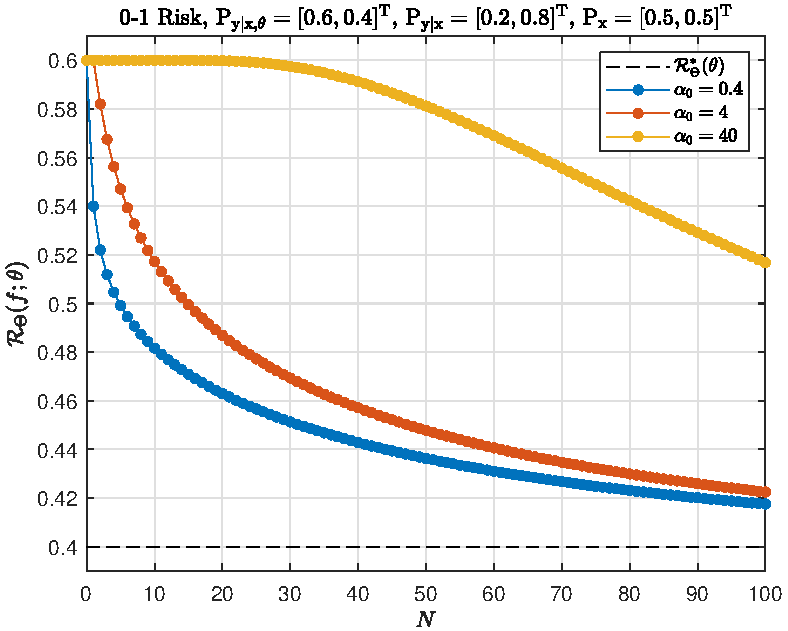
\includegraphics[width=0.7\linewidth]{Risk_cond_01_Dir_N_leg_a0__subj_bad.pdf}
\caption{Excess conditional probability of error, poorly-matched informative Dirichlet-based classifier}
\label{fig:Risk_cond_01_Dir_N_leg_a0__subj_bad}
\end{figure}

Also, it is important to consider how a given classifier performs for varying models $\theta$. Figures \ref{fig:Risk_cond_ex_01_Dir_theta__uni} and \ref{fig:Risk_cond_ex_01_Dir_theta__subj} demonstrate the excess conditional probability of error achieved by the conditional majority decision (based on a non-informative Dirichlet prior) and by a classifier derived from an informative Dirichlet prior, respectively. Note that while the former has fewer models for which the error is critically high, the latter has more models for which the clairvoyant risk $\Rcal_{\Theta}^*(\theta)$ is achieved. This a fundamental trade-off between Bayesian learners based on non-informative versus informative priors.
\begin{figure}
\centering
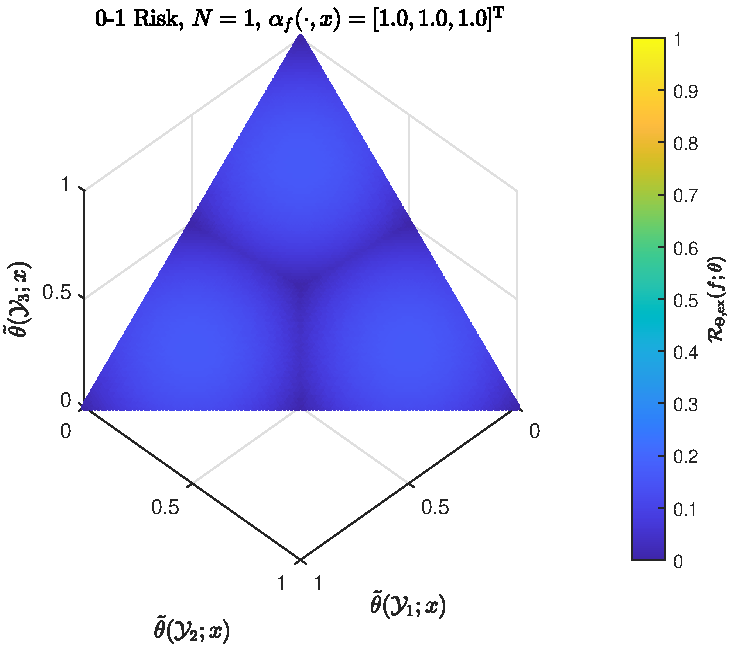
\includegraphics[width=0.7\linewidth]{Risk_cond_ex_01_Dir_theta__uni.pdf}
\caption{Excess conditional probability of error, conditional majority decision}
\label{fig:Risk_cond_ex_01_Dir_theta__uni}
\end{figure}
%
\begin{figure}
\centering
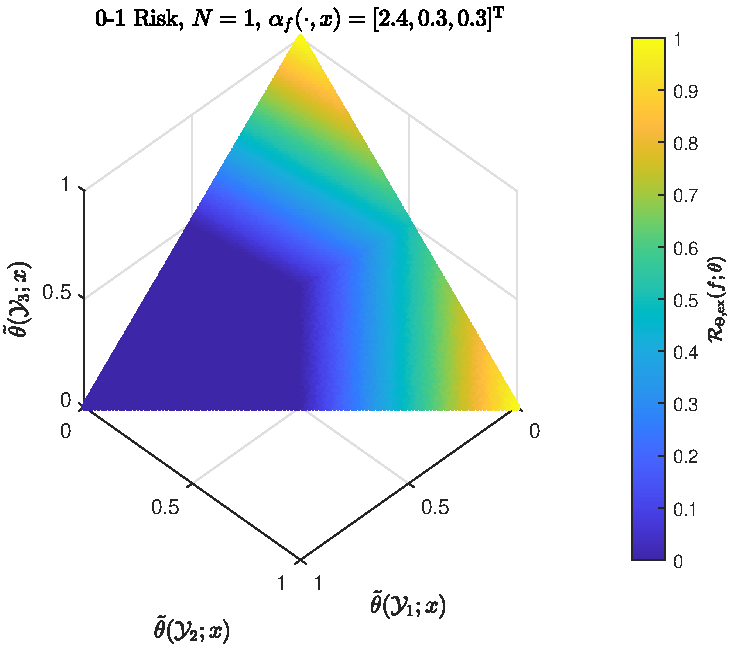
\includegraphics[width=0.7\linewidth]{Risk_cond_ex_01_Dir_theta__subj.pdf}
\caption{Excess conditional probability of error, informative Dirichlet-based classifier}
\label{fig:Risk_cond_ex_01_Dir_theta__subj}
\end{figure}












\section{Plan for Completion}

To complete the thesis, additional work is required in some key areas. Most importantly, additional theory needs to be set down for Bayesian learning with prior distributions of limited support. Subsequently, specific low-dimensionality priors will be used to for decision functions for human recognition tasks, exploiting insights into which models are sensible. Additionally, the established framework will be extended for uncountably infinite sets and joint decisions based on multiple simultaneous observations. 


\subsection{Perform additional research into Bayesian learning with limited-support priors}

The primary contention of this proposal is that all machine learning either explicitly or implicitly depends on prior knowledge imparted by the designer. It is suggested that highly informative prior distributions are required to achieve near-optimal performance for Bayesian approaches when training data is limited; furthermore, it is hypothesized that the specificity of the prior should be expressed using support of relatively low intrinsic dimensionality. These designs enable high performance learning (if the prior support is well chosen) while also keeping the computational complexity of the resulting algorithms sufficiently low, which is a primary concern for practical implementation. 

As such, one of the main thrusts for continued investigation is to analyze the consequences of limited-dimension prior distributions with $\dim(\Theta) = M-1 < |\Ycal||\Xcal| - 1$. Initial research will continue with the assumption that the sets $\Xcal$ and $\Ycal$ are finite, promoting simplicity and explainable results. Trade studies will be performed to assess how the reduced support dimensionality $M-1$ and mismatch from the true model $\theta$ affect the achievable risk. Additional focus will be put on asymptotic trends with training data volume $N$ - unlike predictive distributions based on full-support priors, those derived from limited-support priors will certainly not be asymptotically consistent estimators of $\theta$ in general and thus the clairvoyant risk may never be met. 

A class of low-dimensional prior that will be of specific interest is the class of mixture models satisfying
\begin{equation}
\uptheta \equiv \sum_{m = 1}^M h_m \upphi_m \;,
\end{equation}
such that the data-generating model $\theta$ is a convex combination of distributions $h_m \in \Theta$. In such a case, the convex coefficients $\phi$ are referred to as ``hyperparameters'' - an obvious choice for statistical characterization of these coefficients is, again, the Dirichlet PDF. It will be shown that if the mixture distributions $h_m$ have disjoint support, such that
\begin{equation}
h_i(y,x) \cdot h_j(y,x) = 0, \quad \forall \; (y,x) \in \Ycal \times \Xcal, \quad \forall \; i,j \;,
\end{equation}
then a Dirichlet PDF $\prm_{\upphi}$ for the hyperparameters is a conjugate prior for the training data likelihood function and closed-support posterior distributions can be realized.





\subsection{Assess performance of low-dimensional support Bayesian learners on human recognition applications}

Having developed Bayesian inference methods based on limited-dimensionality priors, the goal will be to successfully demonstrate performance on human recognition tasks. Simulated binary classification data mimicking audiovisual recordings will be used first for proof-of-concept; data drawn from the set $\Xcal = \{0,1\}^K$ will be used, first with singular $K$ and then a multi-index $K$ to approximate audio records and images, respectively. To demonstrate a property characteristic of such data, distinct patterns will be generated and subjected to random translations and rotations; Figure \ref{fig:character_sim_ex} shows example image data.
\begin{figure}
\centering
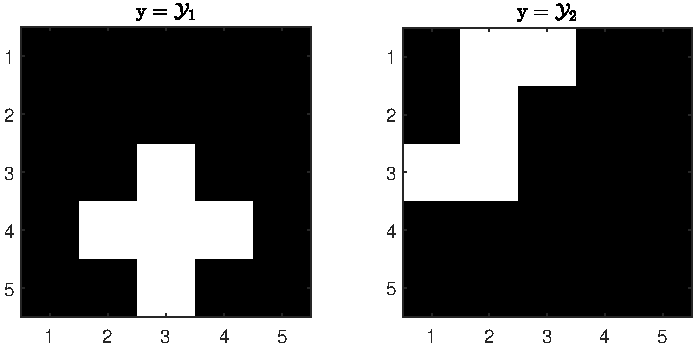
\includegraphics[width=0.8\linewidth]{character_sim_ex.pdf}
\caption{Simulated character recognition data}
\label{fig:character_sim_ex}
\end{figure}

This problem clearly exhibits the human-recognition task properties discussed in Section \ref{sec:approach}. First, note that the marginal model $\theta': \Xcal \mapsto \Rbb_{\geq 0}$ is clearly non-zero for only select values $\xrm = x$; for the data shown, only $9+2(9) = 27$ images $x$ will ever be observed, rather than the $2^{25} = 33554432$ possible binary images. Second, it should be clear that none of the images $x$ that can be generated when $\yrm = \Ycal_1$ would ever occur when $\yrm = \Ycal_2$, and visa-versa. As such, the conditional models must satisfy $\big\| \tilde{\theta}(x) \big\|_{\infty} = 1$ and the clairvoyant risk for this problem should be zero.

By using appropriate limited-support prior distributions, it is expected that low probability of error will be realizable even with limited training data and no \emph{a priori} understanding of the patterns used. After successful demonstration, the problem size will be increased, such that training data volume becomes more critical and prior knowledge more important. The decision functions will subsequently be tested on real-world data such as the optical character recognition data \cite{lecun-mnist} exemplified in Figure \ref{fig:mnist_digit_ex}.
 




\subsection{Extend existing results for uncountably infinite sets}

The preliminary work assumes that the data pairs $(\yrm,\xrm)$ are drawn from a finite set $\Ycal \times \Xcal$. As mentioned, essentially all modern machine learning algorithms are deployed on digital processors and thus this characterization of the data is not presumptuous - even if the cardinalities of the sets are immense, the sets will undoubtedly be finite if the data is to be stored using a digital representation. However, as many digital records of interest for regression and classification are made by sampling continuous physical phenomena (acoustic fluctuations, electromagnetic waves, etc.), a complete learning theory must include an extension to continuous spaces. An analogous case can be found in harmonic analysis - certainly our understanding of the digital Fourier transform has benefited from study of the continuous Fourier transform.

With this in consideration, the initial work will be generalized for Euclidean spaces $\Ycal$ and $\Xcal$ (starting with $\Ycal = \Xcal = \Rbb$) and the joint distribution $\theta$ will be treated as a probability density function. As the set of PDF's $\Pcal(\Theta)$ is infinite-dimensional, an explicit prior distribution $\prm_{\uptheta}$ cannot be defined over this space. Instead, the model $\uptheta$ is treated as a random process. The empirical distribution is now defined as $\bar{N}(\Drm) = \sum_{n=1}^N \delta\left( \cdot - \Drm_n \right)$ on its Euclidean domain.

For the preliminary work on learning with full-support Dirichlet priors, generalization efforts have already been started, treating the model as a continuous Dirichlet process $\uptheta \sim \DP(\alpha)$. Inheriting all the desirable properties of the Dirichlet distribution, is is straight-forward to formulate the posterior model process $\uptheta | \nbarrm \sim \DP(\alpha+\nbarrm)$ and the Bayesian predictive PDF for novel observations. To enable analyses similar to those performed for finite data sets, the concepts of the multinomial process and Dirichlet-multinomial process are introduced, inheriting properties from their corresponding PMF's over finite domains. 

After using the Dirichlet process to investigate Bayesian learning with ``full support'' prior knowledge, the limited-support prior results from the finite set case will be generalized as well. Although typically not described as such, this is the type of problem setup assumed by most existing Bayesian parametric learning methods. As before, the continuous model $\theta$ will be treated as a mixture of a finite number of distributions $h_m$ and the finite-dimensional ``support'' of the model will be characterized by hyperparameters $\phi$.




\subsection{Extend framework for semi-supervised joint decisions based on multiple observations}

In the preliminary work, Bayesian decisions are made using the model posterior $\prm_{\tilde{\uptheta} | \xrm,\Drm}$. Under the Dirichlet prior assumption, it has been shown that the predictive models $\tilde{\uptheta}(x)$ are conditionally independent of the novel observation $\xrm$ given the training data $\Drm$. In general this will not be the case. As such, the use of $\xrm$ to refine our statistical understanding of the model distribution can be viewed as a \emph{semi-supervised} learning procedure. Semi-supervised learning is of interest in machine learning research - labeled data can be costly to obtain, while unlabeled data is in abundance. 

The current results design the decision function and assess the risk for a single decision $h \in \Hcal$ based on a single observation $\xrm = x$. To enable a more meaningful investigation of semi-supervised learning potential, the existing work will be generalized for $L$ joint decisions $(h_1,\ldots,h_L) \in \Hcal^L$ based on observations $(\xrm_1,\ldots,\xrm_L) \in \Xcal^L$, each corresponding to a distinct unobserved random element $(\yrm_1,\ldots,\yrm_L) \in \Ycal^L$. The loss function will generalize as the sum of the losses incurred by each decision, $\Lcal(h,y) = \sum_{l=1}^L \Lcal_0(h_l,y_l)$. This setup also enables a direct comparison of the resultant Bayesian decision functions with non-probabilistic learners that are designed with empirical risk minimization over a training set and are assessed with empirical risk on a reserved test set.

It is straightforward to show that using a Dirichlet prior, the model will again be conditionally independent of the novel observations and thus the decisions will be made independently using the Bayesian predictive distribution $\mu_{\tilde{\uptheta} | \Drm}$. Consequently, each decision $h_l$ will be dependent solely on the observation $x_l$.

Moving away from Dirichlet priors to distributions with statistical dependency between $\uptheta'$ and $\tilde{\uptheta}$, each specific decision $h_l$ will be dependent on all the novel observations $(\xrm_1,\ldots,\xrm_L)$, not just the corresponding observation. How the risk trends with the number of novel observations $L$ will be of interest; it can be shown that the novel observations refine the posterior distribution of $\uptheta'$ and consequently, the posterior of the predictive model $\tilde{\uptheta}$.








\newpage
\appendix



\section{Dirichlet random process conditioned on its aggregation}
\label{app:Dir_agg}

This section details an important property of Dirichlet distributed random processes. The following development first considers Dirichlet random processes over a countable domain and then generalizes for continuous-domain Dirichlet processes. 

First, define the PDF of a Dirichlet aggregation \cite{ferguson}. Let the random process $\uptheta \in \Theta = \Pcal(\Ycal)$ be Dirichlet over the countable set $\Ycal$ with parameterizing function $\alpha \in {\Rbb^+}^{\Ycal}$. Define an arbitrary partition of $\Ycal$: $\left\{ \ldots,\Scal(z),\ldots \right\}$, $z \in \Zcal$; the aggregation $\uptheta' \in \Pcal(\Zcal)$, $\uptheta'(z) \equiv \sum_{y \in \Scal(z)} \uptheta(y)$ is thus also Dirichlet and has a parameterizing function $\alpha' \in {\Rbb^+}^{\Zcal}$, $\alpha'(z) \equiv \sum_{y \in \Scal(z)} \alpha(y)$.

The PDF of the original random process $\uptheta$ conditioned on its aggregation $\uptheta'$ can be formulated as
\begin{IEEEeqnarray}{rCl}
\prm_{\uptheta | \uptheta'}(\theta | \theta') & = & \frac{\beta(\alpha') \prod_{y \in \Ycal} \theta(y)^{\alpha(y)-1}}{\beta(\alpha) \prod_{z \in \Zcal} \theta'(z)^{\alpha'(z)-1}} \\
& = & \prod_{z \in \Zcal} \Bigg[ \beta\Big( \big\{ \alpha(y) : y \in \Scal(z) \big\} \Big)^{-1} \frac{\prod_{y \in \Scal(z)} \theta(y)^{\alpha(y)-1}}{\theta'(z)^{\alpha'(z)-1}} \Bigg] \nonumber \\ 
& = & \prod_{z \in \Zcal} \Bigg[ \frac{\theta'(z)^{1-|\Scal(z)|}}{\beta\Big( \big\{ \alpha(y) : y \in \Scal(z) \big\} \Big)} \prod_{y \in \Scal(z)} \left(\frac{\theta(y)}{\theta'(z)}\right)^{\alpha(y)-1} \Bigg] \nonumber \;,
\end{IEEEeqnarray}
which is defined for $\left\{ \theta \in {\Rbb_{\geq 0}}^{\Ycal} : \sum_{y \in \Scal(z)} \theta(y) = \theta'(z), \quad \forall z \in \Zcal \right\}$.

Observe that the partitioned segements are conditionally independent; introduce subscript notation to refer to the function segment $\uptheta_z = \big\{ \uptheta(y): y \in \Scal(z) \big\}$. The PDF $\prm_{\uptheta | \uptheta'}$ can now be decomposed as $\prm_{\uptheta | \uptheta'}(\ldots,\theta_z,\ldots | \theta') = \prod_{z \in \Zcal} \prm_{\uptheta_z | \uptheta'(z)}\big( \theta_z | \theta'(z) \big)$

Next, normalize the segments of $\uptheta$ to form $\tilde{\uptheta} = \big( \ldots,\tilde{\uptheta}_z,\ldots \big)$, where $\tilde{\uptheta}_z \equiv \uptheta_z / \uptheta'(z)$, and formulate the conditional PDF
\begin{IEEEeqnarray}{rCl}
\prm_{\tilde{\uptheta} | \uptheta'}\left( \tilde{\theta} | \theta' \right) & = & \prod_{z \in \Zcal} \Bigg[ \frac{\prod_{y \in \Scal(z)} \tilde{\theta}_z(y)^{\alpha(y)-1}}{\beta\Big( \big\{ \alpha(y) : y \in \Scal(z) \big\} \Big)} \Bigg] \\
& = & \prod_{z \in \Zcal} \Dir\Big( \tilde{\theta}_z ; \big\{ \alpha(y) : y \in \Scal(z) \big\} \Big) \nonumber \;.
\end{IEEEeqnarray}
which is defined for $\tilde{\theta} \in \prod_{z \in \Zcal} \left\{ \tilde{\theta}_z \in \Pcal\big(\Scal(z)\big) \right\}$. Thus after conditioning, the normalized segments $\tilde{\uptheta}_z$ are Dirichlet distributed, independent of one another, and independent of the aggregation $\uptheta'$. This principle holds for continuous-domain Dirichlet processes $\uptheta$ as well - the segments $\tilde{\uptheta}_z$ are now continuous-domain Dirichlet processes.








\section{Multinomial Distribution Properties}
\label{app:mult}

\subsection{Aggregation}

A characteristic of a Multinomial random process is that its aggregations are also Multinomial \cite{johnson}. Consider a random process $\bar{\nrm} \sim \Multi(N,\theta)$ over the set $\Ycal$. Define an arbitrary partition of $\Ycal$: $\left\{ \ldots,\Scal(z),\ldots \right\}$, $z \in \Zcal$; the transformed random process $\nrm'(z) \equiv \sum_{y \in \Scal(z)} \bar{\nrm}(y)$ is distributed as $\nrm' \sim \Multi(N,\theta')$ with parameterizing function $\theta'(z) = \sum_{y \in \Scal(z)} \theta(y)$.

To prove this principle, define the subset $\tilde{\Ncal} = \big\{ \bar{n} \in \Ncal : \sum_{y \in \Scal(z)} \bar{n}(y) = n'(z), \quad \forall z \in \Zcal \big\} \subseteq \bar{\Ncal}$, where the original random process $\bar{\nrm} \in \bar{\Ncal}$. Next, observe
\begin{IEEEeqnarray}{rCl}
\Prm_{\mathrm{n}'}(n') & = & \sum_{\bar{n} \in \tilde{\Ncal}} \Prm_{\nbarrm}(\bar{n}) \\
& = & \Mcal(n') \prod_{z \in \Zcal} \sum_{\substack{n'(z) = \\ \sum_{y \in \Scal(z)} \bar{n}(y)}} \Mcal\big( \{ \bar{n}(y): y \in \Scal(z) \} \big) \prod_{y \in \Scal(z)} \theta(y)^{\bar{n}(y)} \nonumber \\
& = & \Mcal(n') \prod_{z \in \Zcal} \theta'(z)^{n'(z)} = \Multi(n' ; N,\theta') \nonumber \;,
\end{IEEEeqnarray}
where the multinomial theorem \cite{graham} has been used.




\subsection{Conditioned on its Aggregation}

If the multinomial random process $\bar{\nrm}$ is conditioned on its aggregation over the partition $\left\{ \ldots,\Scal(z),\ldots \right\}$, $z \in \Zcal$, the distinct segements $\bar{\nrm}(y)$, $y \in \Scal(z)$ become independent multinomial random processes,
\begin{IEEEeqnarray}{rCl}
\Prm_{\bar{\nrm} | \nrm'}(\bar{n} | n') & = & \frac{\Mcal(\bar{n}) \prod_{y \in \Ycal} \theta(y)^{\bar{n}(y)}}{\Mcal(n') \prod_{z \in \Zcal} \theta'(z)^{n'(z)}} \\
& = & \prod_{z \in \Zcal} \Bigg[ \Mcal\Big( \big\{ \bar{n}(y) : y \in \Scal(z) \big\} \Big) \prod_{y \in \Scal(z)} \left(\frac{\theta(y)}{\theta'(z)}\right)^{\bar{n}(y)} \Bigg] \nonumber \\
& = & \prod_{z \in \Zcal} \Bigg[ \Mcal\Big( \big\{ \bar{n}(y) : y \in \Scal(z) \big\} \Big) \prod_{y \in \Scal(z)} \tilde{\theta}_z(y)^{\bar{n}(y)} \Bigg] \nonumber \\
& = & \prod_{z \in \Zcal} \Multi\Big( \big\{ \bar{n}(y) : y \in \Scal(z) \big\} ; n'(z) , \big\{ \tilde{\theta}_z(y) : y \in \Scal(z) \big\} \Big) \nonumber \;,
\end{IEEEeqnarray}
on the domain $\left\{ \bar{n} \in {\Zbb_{\geq 0}}^{\Ycal} : \sum_{y \in \Scal(z)} \bar{n}(y) = n'(z), \quad \forall z \in \Zcal \right\}$. Observe that the segment over the set $\Scal(z)$ sums to $\nrm'(z)$ and is parameterized by the normalized segment $\tilde{\theta}_z \equiv \big\{ \theta(y)/\theta'(z) : y \in \Scal(z) \big\}$.





\section{Dirichlet-Multinomial random process conditioned on its aggregation} 
\label{app:DM_agg}

A defining characteristic of a Dirichlet-Multinomial random process is that its aggregations are also Dirichlet-Multinomial \cite{johnson}. Consider a DM random process $\bar{\nrm} \sim \DM(N,\alpha)$ over the set $\Ycal$. Define an arbitrary partition of $\Ycal$: $\left\{ \ldots,\Scal(z),\ldots \right\}$, $z \in \Zcal$; the transformed random process $\nrm'(z) \equiv \sum_{y \in \Scal(z)} \bar{\nrm}(y)$ is neccessarily Dirichlet-Multinomial with parameterizing function $\alpha'(z) = \sum_{y \in \Scal(z)} \alpha(y)$.

It can be shown that conditioned on the aggregation $\nrm'$, the segments $\big\{ \bar{\nrm}(y) : y \in \Scal(z) \big\}$ of the original random process become independent Dirichlet-Multinomial random processes, such that
\begin{IEEEeqnarray}{rCl}
\Prm_{\bar{\nrm} | \nrm'}(\bar{n} | n') & = & \frac{\Mcal(\bar{n}) \beta(\alpha)^{-1} \beta(\alpha+\bar{n})}{\Mcal(n') \beta(\alpha')^{-1} \beta(\alpha'+n')} \\
& = & \left( \prod_{z \in \Zcal} \frac{\Gamma\big( \alpha'(z)+n'(z) \big)}{n'(z)! \Gamma\big( \alpha'(z) \big)} \right)^{-1} \left( \prod_{y \in \Ycal} \frac{\Gamma\big( \alpha(y)+\bar{n}(y) \big)}{\bar{n}(y)! \Gamma\big( \alpha(y) \big)} \right) \nonumber \\
& = & \prod_{z \in \Zcal} \left[ \frac{n'(z)! \Gamma\big( \alpha'(z) \big)}{\Gamma\big( \alpha'(z)+n'(z) \big)} \prod_{y \in \Scal(z)} \frac{\Gamma\big( \alpha(y)+\bar{n}(y) \big)}{\bar{n}(y)! \Gamma\big( \alpha(y) \big)} \right] \nonumber \\
& = & \prod_{z \in \Zcal} \DM\Big( \big\{ \bar{n}(y) : y \in \Scal(z) \big\} ; n'(z), \big\{ \alpha(y) : y \in \Scal(z) \big\} \Big) \nonumber \;,
\end{IEEEeqnarray}
on the domain $\left\{ \bar{n} \in {\Zbb_{\geq 0}}^{\Ycal} : \sum_{y \in \Scal(z)} \bar{n}(y) = n'(z), \quad \forall z \in \Zcal \right\}$. 








\newpage

\bibliographystyle{plain}
\bibliography{{../References/phd_bib}}

\end{document}


























